\documentclass[a4paper,11pt]{book}
%\documentclass[a4paper,twoside,11pt,titlepage]{book}
\usepackage{listings}
\usepackage[utf8]{inputenc}
\usepackage[spanish]{babel}

\usepackage{tgpagella}
\usepackage[T1]{fontenc}

\usepackage{textcomp}

% \usepackage[style=list, number=none]{glossary} %
%\usepackage{titlesec}
%\usepackage{pailatino}

%\decimalpoint
\usepackage{dcolumn}
\newcolumntype{.}{D{.}{\esperiod}{-1}}
\makeatletter
\addto\shorthandsspanish{\let\esperiod\es@period@code}
\makeatother


%\usepackage[chapter]{algorithm}
\RequirePackage{verbatim}
%\RequirePackage[Glenn]{fncychap}
\usepackage{fancyhdr}
\usepackage{graphicx}
\usepackage{afterpage}

\usepackage{longtable}

\usepackage[pdfborder={000}]{hyperref} %referencia

\usepackage{tabularx}
\usepackage{xspace}

% ********************************************************************
% Re-usable information
% ********************************************************************
\newcommand{\myTitle}{Bot de Telegram para la gestión de bandas\xspace}
\newcommand{\myDegree}{Grado en Ingeniería Informática\xspace}
\newcommand{\myName}{Daniel Haro Contreras\xspace}
\newcommand{\myProf}{Rosana Montes Soldado\xspace}
%\newcommand{\mySupervisor}{Put name here\xspace}
\newcommand{\myFaculty}{Escuela Técnica Superior de Ingenierías Informática y de Telecomunicación\xspace}
\newcommand{\myFacultyShort}{E.T.S. de Ingenierías Informática y de
Telecomunicación\xspace}
\newcommand{\myDepartment}{Departamento de Lenguajes y Sistemas Informáticos\xspace}
\newcommand{\myUni}{\protect{Universidad de Granada}\xspace}
\newcommand{\myLocation}{Granada\xspace}
\newcommand{\myTime}{\today\xspace}
\newcommand{\myVersion}{Version 0.1\xspace}

\hypersetup{
pdfauthor = {\myName (email (en) ugr (punto) es)},
pdftitle = {\myTitle},
pdfsubject = {},
pdfkeywords = {palabra_clave1, palabra_clave2, palabra_clave3, ...},
pdfcreator = {LaTeX con el paquete ....},
pdfproducer = {pdflatex}
}

%\hyphenation{}

\usepackage{multirow}
\usepackage{makecell}
%\usepackage{doxygen/doxygen}
%\usepackage{pdfpages}
\usepackage{url}
\usepackage{colortbl,longtable}
\usepackage[stable]{footmisc}
%\usepackage{index}

%\makeindex
%\usepackage[style=long, cols=2,border=plain,toc=true,number=none]{glossary}
% \makeglossary

% Definición de comandos que me son tiles:
%\renewcommand{\indexname}{Índice alfabético}
%\renewcommand{\glossaryname}{Glosario}

\pagestyle{fancy}
\fancyhf{}
\fancyhead[LO]{\leftmark}
\fancyhead[RE]{\rightmark}
\fancyhead[RO,LE]{\textbf{\thepage}}
\renewcommand{\chaptermark}[1]{\markboth{\textbf{#1}}{}}
\renewcommand{\sectionmark}[1]{\markright{\textbf{\thesection. #1}}}

\setlength{\headheight}{1.5\headheight}

\newcommand{\HRule}{\rule{\linewidth}{0.5mm}}
%Definimos los tipos teorema, ejemplo y definición podremos usar estos tipos
%simplemente poniendo \begin{teorema} \end{teorema} ...
\newtheorem{teorema}{Teorema}[chapter]
\newtheorem{ejemplo}{Ejemplo}[chapter]
\newtheorem{definicion}{Definición}[chapter]

\definecolor{gray97}{gray}{.97}
\definecolor{gray75}{gray}{.75}
\definecolor{gray45}{gray}{.45}
\definecolor{gray30}{gray}{.94}

\lstset{ frame=Ltb,
     framerule=0.5pt,
     aboveskip=0.5cm,
     framextopmargin=3pt,
     framexbottommargin=3pt,
     framexleftmargin=0.1cm,
     framesep=0pt,
     rulesep=.4pt,
     backgroundcolor=\color{gray97},
     rulesepcolor=\color{black},
     %
     stringstyle=\ttfamily,
     showstringspaces = false,
     basicstyle=\scriptsize\ttfamily,
     commentstyle=\color{gray45},
     keywordstyle=\bfseries,
     %
     numbers=left,
     numbersep=6pt,
     numberstyle=\tiny,
     numberfirstline = false,
     breaklines=true,
   }
 
% minimizar fragmentado de listados
\lstnewenvironment{listing}[1][]
   {\lstset{#1}\pagebreak[0]}{\pagebreak[0]}

\lstdefinestyle{CodigoC}
   {
	basicstyle=\scriptsize,
	frame=single,
	language=C,
	numbers=left
   }
\lstdefinestyle{CodigoC++}
   {
	basicstyle=\small,
	frame=single,
	backgroundcolor=\color{gray30},
	language=C++,
	numbers=left
   }

 
\lstdefinestyle{Consola}
   {basicstyle=\scriptsize\bf\ttfamily,
    backgroundcolor=\color{gray30},
    frame=single,
    numbers=none
   }


\newcommand{\bigrule}{\titlerule[0.5mm]}


%Para conseguir que en las páginas en blanco no ponga cabecerass
\makeatletter
\def\clearpage{%
  \ifvmode
    \ifnum \@dbltopnum =\m@ne
      \ifdim \pagetotal <\topskip
        \hbox{}
      \fi
    \fi
  \fi
  \newpage
  \thispagestyle{empty}
  \write\m@ne{}
  \vbox{}
  \penalty -\@Mi
}
\makeatother

\usepackage{pdfpages}

\begin{document}

% Cambiar Cuadros por Tablas y lista de tablas
\renewcommand{\listtablename}{Índice de tablas}
\renewcommand{\tablename}{Tabla}

\begin{titlepage}
 
 
\newlength{\centeroffset}
\setlength{\centeroffset}{-0.5\oddsidemargin}
\addtolength{\centeroffset}{0.5\evensidemargin}
\thispagestyle{empty}

\noindent\hspace*{\centeroffset}\begin{minipage}{\textwidth}

\centering

\includegraphics[width=\textwidth]{imagenes/logo_ugr.pdf}\\[1.4cm]

\textsc{ \Large TRABAJO FIN DE GRADO\\[0.2cm]}
\textsc{ Grado en Ingeniería Informática }\\[1cm]
% Upper part of the page
% 
% Title
{\Huge\bfseries \myTitle \\
}
\noindent\rule[-1ex]{\textwidth}{3pt}\\[3.5ex]
{\large\bfseries Subtitulo del Proyecto}
\end{minipage}

\vspace{2.5cm}
\noindent\hspace*{\centeroffset}\begin{minipage}{\textwidth}
\centering

\textbf{Autor}\\ {Daniel Haro Contreras}\\[2.5ex]
\textbf{Directora}\\
{\myProf}\\[1cm]

\includegraphics[width=0.3\textwidth]{imagenes/etsiit_logo.png}\\[0.1cm]
\textsc{Escuela Técnica Superior de Ingenierías Informática y de Telecomunicación}\\
\textsc{---}\\
Granada, julio de 2022
\end{minipage}
%\addtolength{\textwidth}{\centeroffset}
%\vspace{\stretch{2}}
\end{titlepage}



\chapter*{}
%\thispagestyle{empty}
%\cleardoublepage

%\thispagestyle{empty}

\begin{titlepage}
 
 
\setlength{\centeroffset}{-0.5\oddsidemargin}
\addtolength{\centeroffset}{0.5\evensidemargin}
\thispagestyle{empty}

\noindent\hspace*{\centeroffset}\begin{minipage}{\textwidth}

\centering
%
\includegraphics[width=0.9\textwidth]{imagenes/logo_ugr.jpg}\\[1.4cm]

%\textsc{ \Large PROYECTO FIN DE CARRERA\\[0.2cm]}
%\textsc{ INGENIERÍA EN INFORMÁTICA}\\[1cm]
% Upper part of the page
% 

 \vspace{3.3cm}

%si el proyecto tiene logo poner aquí

\includegraphics{imagenes/logo.png} 
 \vspace{0.5cm}

% Title

{\Huge\bfseries \myTitle\\
}
\noindent\rule[-1ex]{\textwidth}{3pt}\\[3.5ex]
{\large\bfseries Subtítulo del proyecto.\\[4cm]}
\end{minipage}

\vspace{2.5cm}
\noindent\hspace*{\centeroffset}\begin{minipage}{\textwidth}
\centering

\textbf{Autor}\\ {\myName}\\[2.5ex]
\textbf{Directora}\\
{\myProf}\\[2cm]
%
\includegraphics[width=0.15\textwidth]{imagenes/tstc.png}\\[0.1cm]
%\textsc{Departamento de Teoría de la Señal, Telemática y Comunicaciones}\\
%\textsc{---}\\
%Granada, mes de 201
\end{minipage}
%\addtolength{\textwidth}{\centeroffset}
\vspace{\stretch{2}}

 
\end{titlepage}






\cleardoublepage
\thispagestyle{empty}

\begin{center}
{\large\bfseries \myTitle: Subtítulo del proyecto}\\
\end{center}
\begin{center}
\myName\\
\end{center}

%\vspace{0.7cm}
\noindent{\textbf{Palabras clave}: Telegram, bot, gestión, música, banda}\\

\vspace{0.7cm}
\noindent{\textbf{Resumen}}\\

Poner aquí el resumen.
\cleardoublepage


\thispagestyle{empty}


\begin{center}
{\large\bfseries Project Title: Project Subtitle}\\
\end{center}
\begin{center}
First name, Family name (student)\\
\end{center}

%\vspace{0.7cm}
\noindent{\textbf{Keywords}: Keyword1, Keyword2, Keyword3, ....}\\

\vspace{0.7cm}
\noindent{\textbf{Abstract}}\\

Write here the abstract in English.

\chapter*{}
\thispagestyle{empty}

\noindent\rule[-1ex]{\textwidth}{2pt}\\[4.5ex]

Yo, \textbf{Daniel Haro Contreras}, alumno de la titulación TITULACIÓN de la \textbf{Escuela Técnica Superior
de Ingenierías Informática y de Telecomunicación de la Universidad de Granada}, con DNI 76656133P, autorizo la
ubicación de la siguiente copia de mi Trabajo Fin de Grado en la biblioteca del centro para que pueda ser
consultada por las personas que lo deseen.

\vspace{6cm}

\noindent Fdo: Daniel Haro Contreras

\vspace{2cm}

\begin{flushright}
Granada a X de mes de 201 .
\end{flushright}


\chapter*{}
\thispagestyle{empty}

\noindent\rule[-1ex]{\textwidth}{2pt}\\[4.5ex]

D.ª \textbf{\myProf}, Profesor del Área de XXXX del Departamento de Lenguajes y Sistemas Informáticos de la Universidad de Granada.


\vspace{0.5cm}

\textbf{Informa:}

\vspace{0.5cm}

Que el presente trabajo, titulado \textit{\textbf{\myTitle, Subtítulo del proyecto}},
ha sido realizado bajo su supervisión por \textbf{\myName}, y autorizo la defensa de dicho trabajo ante el tribunal
que corresponda.

\vspace{0.5cm}

Y para que conste, expiden y firman el presente informe en Granada a X de mes de 201 .

\vspace{1cm}

\textbf{La directora:}

\vspace{5cm}

\noindent \textbf{\myProf}

\chapter*{Agradecimientos}
\thispagestyle{empty}

       \vspace{1cm}


Poner aquí agradecimientos...


%\frontmatter
\tableofcontents
\listoffigures
\listoftables
%
%\mainmatter
%\setlength{\parskip}{5pt}

\chapter{Introducción}

\section{Motivación y justificación del proyecto}

% ¿Qué necesidad hay?
% ¿Qué problema existe que se quiera resolver?
% ¿Qué mejoras propongo sobre algo ya existente?
% ¿Por qué he elegido esta temática?

Este proyecto intenta dar respuesta a las agrupaciones musicales que demandan una plataforma gratuita y libre para la mejora de su gestión.

En 2018 se contabilizaron unas 6197 agrupaciones musicales en España según el INE \cite{ineNumeroAgrupaciones}, número que se mantiene estable a lo largo de los años.

Cada agrupación musical, definida como ``dos o más personas que, a través de la voz o de instrumentos musicales, interpretan obras musicales pertenecientes a diferentes géneros y estilos'' según la RAE, se compone de distintos miembros, formando una sociedad. Como en todas las sociedades, se necesita cierto orden para poder alcanzar los objetivos, por lo que algunos de los miembros se tienen que encargar de su gestión: el director musical, el director artístico, el presidente de la asociación, el secretario... Siendo la gestión distinta en cada agrupación.

Los miembros de las agrupaciones musicales realizan ensayos periódicamente con el doble objetivo de mejorar su técnica de interpretación y preparar la celebración de eventos, tales como conciertos, certámenes, concursos, pasacalles... En los ensayos y eventos se interpreta una o varias obras musicales.

El director musical de una agrupación musical se encarga de coordinar la interpretación de las obras musicales, así como planificar y preparar los ensayos y eventos. En ocasiones se sustituye o se complementa con el rol de director artístico, visibilizando el hecho de que los eventos a menudo no son puramente musicales, sino que se añaden teatros o espectáculos visuales como bailes o musicales.

Los administradores de la agrupación (habitualmente, junta directiva) se encargan de las labores de administración no musicales, ayudando también al director. Habitualmente entre estos encontramos un presidente, un secretario y un tesorero.

Para interpretar una obra musical, los miembros de la agrupación leen un papel. El papel puede ser de dos tipos: el que lee el director se denomina \textit{partitura}, y es el papel que recoge la música de todos los instrumentos y voces. Por otra parte, cada músico lee su \textit{particella} (también llamada ``parte''), que solo recoge lo que debe interpretar él individualmente.

En los últimos tiempos la gestión de estas agrupaciones se ha realizado de forma manual, consistente en que los administradores, el director y los miembros se comunican mediante un grupo de mensajería sin ningún tipo de automatización.

De esta forma, algunas de las tareas más frecuentes en la administración de la agrupación podrían ser:

\begin{itemize}
    \item Para la asistencia a eventos y ensayos, cada miembro escribe a través de un grupo, o individualmente al director o un administrador, su intención de asistir o no. Esta comunicación previa le es útil para gestionar qué repertorio es mejor ensayar, en qué orden, o si por el contrario es conveniente aplazar o suspender el evento o ensayo.
    \item Para el repertorio, los distintos documentos (partitura y partes) que necesitan los músicos se envían a través de alguna plataforma de almacenamiento en la nube (como Google Drive, OneDrive o Dropbox) o se imprimen en papel físico por los administradores, repartiéndose en un ensayo a los miembros presentes.
    \item Respecto a la comunicación de eventos y ensayos, se realiza por el canal no especializado de comunicación y la responsabilidad de recordarlos debidamente a los miembros antes de su celebración recae en los administradores.
\end{itemize}

Esta gestión manual y dependiente de aplicaciones de comunicación no especializadas deriva en varios problemas:

\begin{itemize}
    \item La probabilidad de error humano aumenta en el momento en el que los administradores son responsables de recordar eventos y gestionar asistencia.
    \item La carga de trabajo de los administradores es mayor dada la responsabilidad de gestión manual que tienen a la hora de organizar un evento.
    \item Se crea una duplicidad de comunicación, ya que los miembros pueden escribir sobre su asistencia al director o a los administradores, pudiendo darse el caso de que finalmente no todos dispongan de los datos necesarios para organizar un ensayo o evento, o que dispongan de datos contradictorios entre sí.
\end{itemize}

Por todos estos problemas derivados de la gestión manual se necesita software dedicado específicamente a este propósito, automatizando la gestión, que sea personalizable a las necesidades de cada agrupación, no implique enormes gastos de uso y sea fácilmente usable por todos los usuarios.

De este modo, el proyecto está justificado por la necesidad de alternativas para mejorar la gestión del gran número de agrupaciones musicales que existen en nuestro país y que no han podido automatizar aún su gestión.

\section{Objetivos}

% - 1 objetivo general pero que concrete lo que se pretende hacer
% - Varios objetivos específicos redactados en infinitivo y con justificación.

Los objetivos de este trabajo se pueden resumir en tres fundamentales:

\begin{itemize}
    \item Por un lado, dar respuesta a los requerimientos de numerosas agrupaciones musicales con un software que les permita automatizar la gestión de eventos, miembros, ensayos, repertorio, etc., y ayudando a una organización más ágil y efectiva.
    \item Por otro lado, investigar hasta qué punto la interfaz de usuario proporcionada por un bot de Telegram es suficiente, competitiva y cómoda para el usuario. Esta interfaz está integrada en un chat, por lo que se pretende identificar las limitaciones que puedan darse, y explorar soluciones que sorteen dichas carencias.
    \item Aportar al conocimiento colectivo aportando guías sobre el desarrollo de un bot de Telegram usando tecnologías actuales.
\end{itemize}

Para el primer objetivo se cumpla de manera satisfactoria, se establecen varios requisitos básicos:

\begin{itemize}
    \item Se debe disponer de una página web donde quede claro qué problemas pretende resolver la herramienta, de modo que las agrupaciones puedan ver las ventajas de su uso. Esta información también debe quedar clara en la propia herramienta.
    \item El uso de la herramienta debe ser lo más sencillo y obvio posible, dada la heterogeneidad de los usuarios, por su edad, profesión, nivel de estudios o grado de implicación en la agrupación.
    \item En el desarrollo de la herramienta se tienen que tener en cuenta los roles de miembro no administrador y quien sí es administrador, de forma que cada rol deberá tener distintas funcionalidades disponibles. Por ejemplo, solo un administrador podrá eliminar a otros miembros.
    \item Se debe buscar el mejor diseño que se pueda ofrecer dentro de las limitaciones de la tecnología escogida, de modo que un mal diseño no haga que los usuarios prefieran volver a la gestión manual.
\end{itemize}


%
\chapter{Estado del arte}

% Descripción de los antecedentes del trabajo.
% Elegir un título apropiado.

\section{Dominio del problema a resolver}

En la actualidad, la digitalización de empresas, administraciones y organismos públicos avanza a ritmo imparable, y la situación excepcional generada por la pandemia de COVID-19 no ha hecho más que afianzar este avance.

Los datos del Índice de Digitalización de la Economía y la Sociedad (DESI) en 2022\cite{desiUE}, índice que monitoriza el rendimiento digital de Europa y el progreso de los países de la Unión Europea en su competitividad digital, muestran que todos los países han progresado en su digitalización. Destaca el hecho de que los países que han empezado en un nivel más bajo de desarrollo digital crecen a un ritmo más rápido, y que numerosos países crecen a un ritmo más elevado del que se les espera, como es el caso de España\cite{desiSpain} (con un 0.7\% más de progreso del esperado).
En concreto, nuestro país es el séptimo con mayor nivel de digitalización según este índice, y el número de personas con competencias digitales básicas es del 64\%, por encima de la media de la UE, del 54\%. Está por encima de la UE también en implementación de la banda ancha fija de al menos 100 Mbps, usuarios de la administración electrónica o pymes con nivel básico de intensidad digital.

%España 2º lugar Índice de Digitalización de la Economía y la Sociedad

%Otras áreas se han modernizado, como todas las empresas. Datos: https://servicioestudiosugt.com/digitalizacion-de-la-empresa-espanola-3-edicion/
A nivel empresarial otros estudios concluyen que la digitalización está más estancada\cite{digitalizacionEmpresaUGT}, debido a una baja inversión en TIC.

%Incluso a nivel de la administración se están impulsando estrategias para avanzar en la digitalización, como España Digital 2026
Por otro lado, a nivel de la administración se están impulsando estrategias para avanzar en la digitalización, como España Digital 2026\cite{espanaDigital2026}, fomentando programas para acelerar la digitalización de pymes (pequeñas y medianas empresas), mejorar la conectividad o 

%Sin embargo, las agrupaciones musicales, que aumentan, siguen sin modernizarse, cuando podrían disfrutar de numerosas ventajas haciendo uso de la tecnología.

Pese a todo esto, algunos sectores de la sociedad aún manifiestan reticencias para proceder a su digitalización, por la falta de herramientas, recursos o ayuda. 
Una de ellas es la que nos ocupa en este trabajo: las asociaciones o agrupaciones musicales. La complejidad de su gestión es suficiente para que los beneficios de la digitalización se puedan manifestar, dada la cantidad de personas que se pueden encontrar en cada una de ellas y la naturaleza de los procesos que siguen, como la programación de ensayos y eventos, la gestión de repertorio o la gestión de miembros.

Por ejemplo, para la correcta planificación de ensayos y eventos, tanto el director como los administradores necesitan conocer con antelación qué músicos tienen pensado asistir y cuáles estarán ausentes. Esto les permitirá saber si se necesita llamar a un músico externo a la agrupación para que participe en un evento, o si es mejor cancelar o aplazar el evento. Para esta tarea, habitualmente el director avisa del evento por un grupo de mensajería a los miembros, y pide que quien no tenga pensado asistir se lo notifique. De este modo se generan varios problemas:

\begin{itemize}
    \item La información sobre qué miembros han notificado su ``no asistencia'' solo la tiene el director, por lo que si otros administradores quieren conocerla se la tienen que pedir individualmente.
    \item Si algún miembro ha comunicado su ``no asistencia'' a otro administrador, tiene que poner la información en común con la del director, pudiendo dar lugar a discrepancias.
    \item Si el director quiere tener la información de asistencia centralizada, tiene que repasar sus conversaciones con los miembros para elaborar una tabla de asistencia, que tiene que ir actualizando manualmente, con la carga de trabajo que ello supone.
\end{itemize}

Similares problemas se crean para los demás procesos que se llevan a cabo en una agrupación musical.

Es evidente, por tanto, que se necesita una herramienta específica que permita automatizar sus procesos y avanzar en su digitalización para equipararla a la del resto de la sociedad.

Aunque ya existen herramientas como Glissandoo, que se analiza en este capítulo, son de pago, poco personalizables o están poco integradas en el flujo de trabajo actual de las agrupaciones. Es por ello que este trabajo pretende aportar una alternativa libre que solucione estos inconvenientes, de modo que:

\begin{itemize}
    \item Cada agrupación pueda montar su propio servidor con la aplicación, personálizandola y adaptándola a sus necesidades.
    \item Los gastos por uso de la herramienta solo dependan del servidor que use la agrupación, si usa un servidor dedicado.
    \item Sea usable en todas las plataformas en las que se pueda acceder a un navegador web.
    \item Esté integrada en una herramienta de mensajería que ya esté en uso como es Telegram, pero añadiendo funcionalidad específica y automática necesaria para la gestión de la agrupación, eximiendo a los administradores y el director de tareas que se pueden automatizar.
\end{itemize}


% Descripción más detallada del problema, carencias que existen,
% características específicas de los usuarios finales, descripción de
% trabajos previos del cual este es una extensión o de proyectos de 
% investigación en el que se enmarca, etc.

\section{Trabajos relacionados}
% Evidencias científicas o revisiones recientes de uso de tecnologías o
% metodologías para resolver un problema igual o similar al mío. Buscar
% referencias en fuentes fiables como Google Scholar.

\section{Aplicaciones similares}
% Descripciones, capturas y tabla comparativa
% Alternativas: Glissandoo, Whatsapp

Aunque aún la mayoría de agrupaciones usan Whatsapp como herramienta de comunicación sin usar ningún software más que automatice las tareas, en los últimos tiempos ha surgido otra herramienta que da respuesta a sus necesidades:

\subsection{Glissandoo}

Glissando (\url{https://glissandoo.com/}) es un software creado por la empresa Plausible Technologies, con sede en Valencia. En su página web se define como ``un software que nace con el objetivo de profesionalizar, modernizar y digitalizar las instituciones musicales''. Incorpora numerosas funcionalidades para digitalizar instituciones musicales, tal y como pretende este trabajo. Entre ellas se encuentran:

\begin{itemize}
    \item Organización de ensayos y conciertos. Los miembros pueden ver los ensayos y conciertos en la página de inicio.
    \item Previsión de asistencia y pasar lista: para cada ensayo o concierto, el miembro puede seleccionar si tiene prevista su asistencia o no.
    \item Distribución de partituras: en la sección de inicio se puede acceder a un listado de todo el repertorio de los ensayos y conciertos programados, y en cada uno de los ensayos se puede ver el repertorio asociado.
    \item Comunicaciones: los administradores pueden añadir avisos que reciben los miembros, teniendo la capacidad de responder, reaccionar, y adjuntar archivos a los comunicados.
\end{itemize}

Se pueden ver varias capturas de la aplicación en la figura \ref{fig:capturas_glissandoo}.
\begin{figure}[h]
\minipage{0.32\textwidth}
  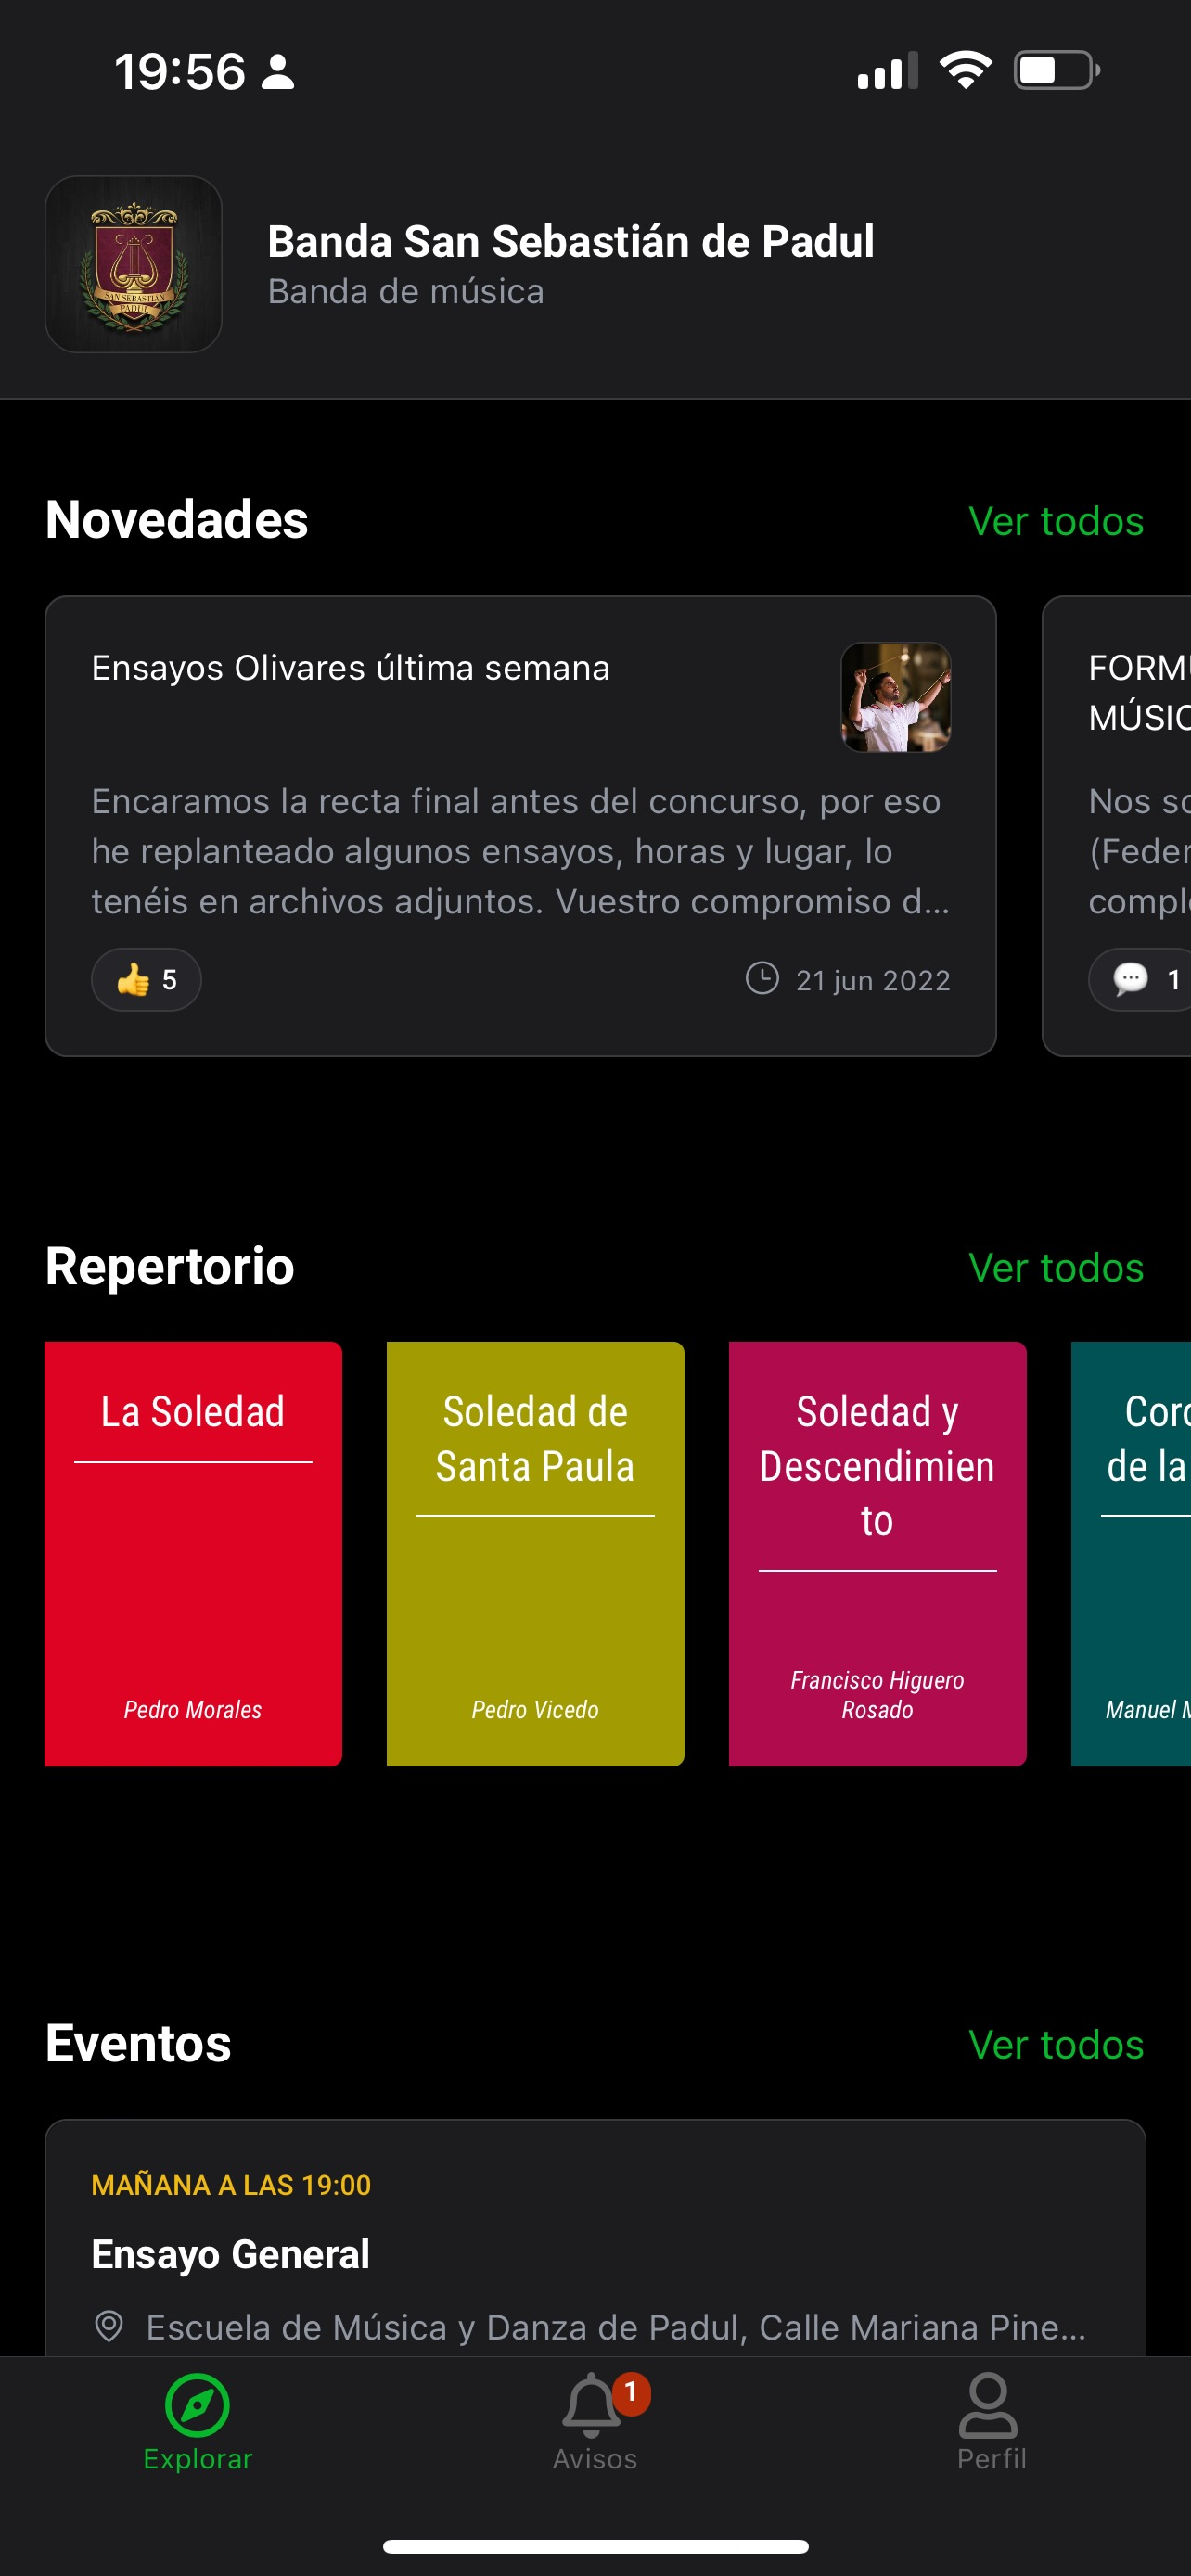
\includegraphics[width=\linewidth]{imagenes/capturas_glissandoo/IMG_0928.jpeg}
\endminipage\hfill
\minipage{0.32\textwidth}
  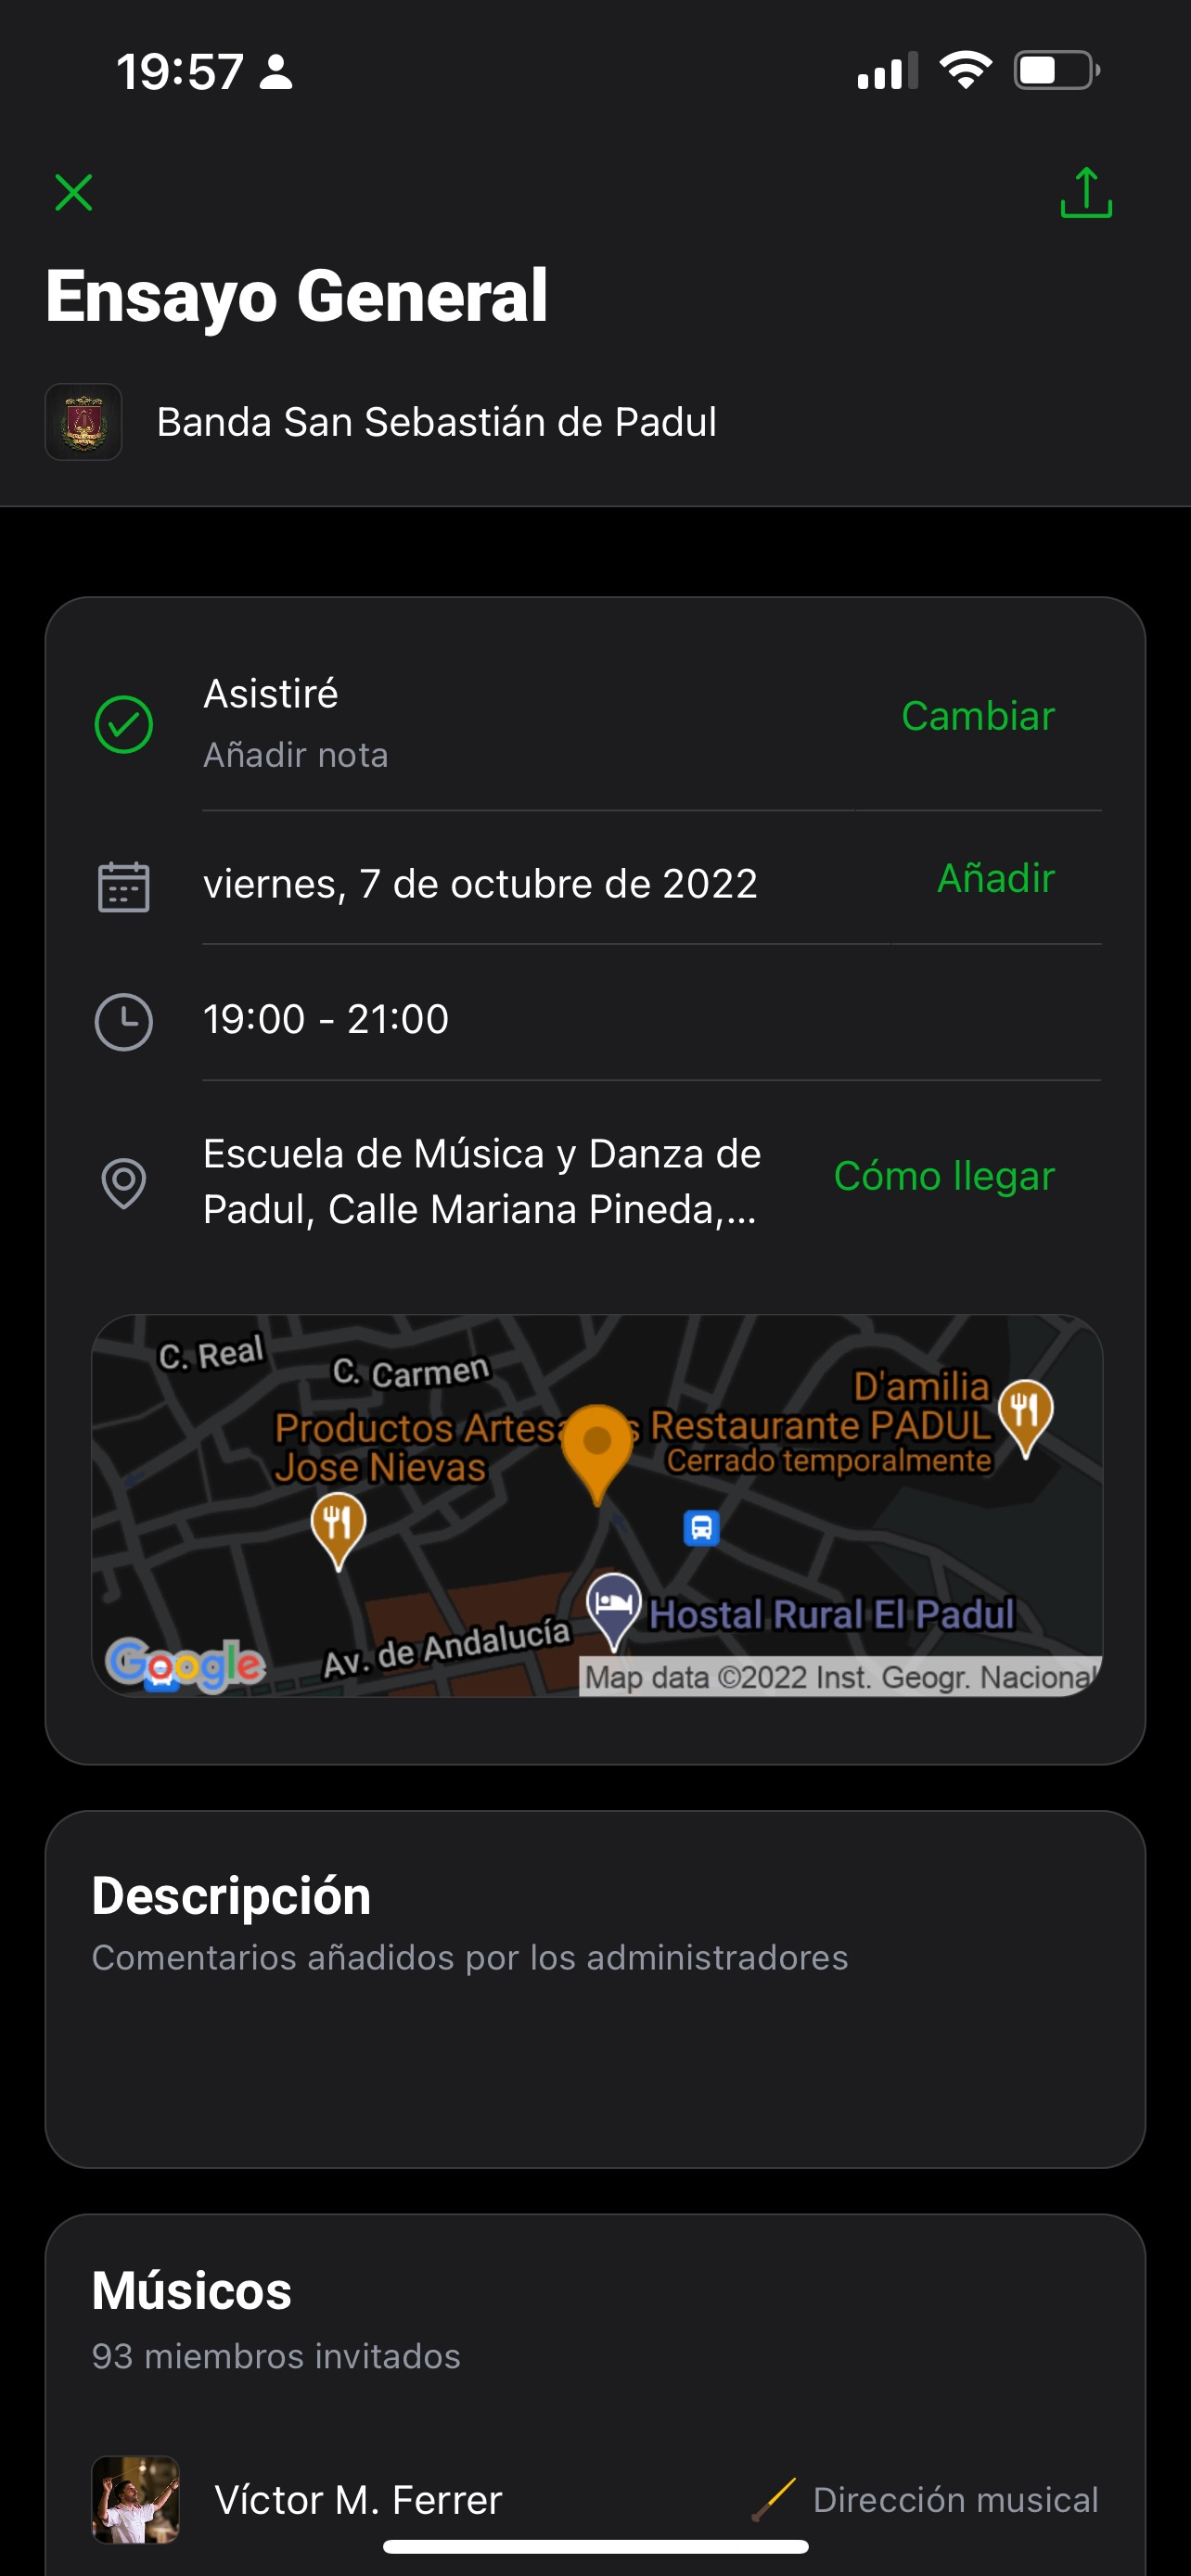
\includegraphics[width=\linewidth]{imagenes/capturas_glissandoo/IMG_0929.jpeg}
\endminipage\hfill
\minipage{0.32\textwidth}
  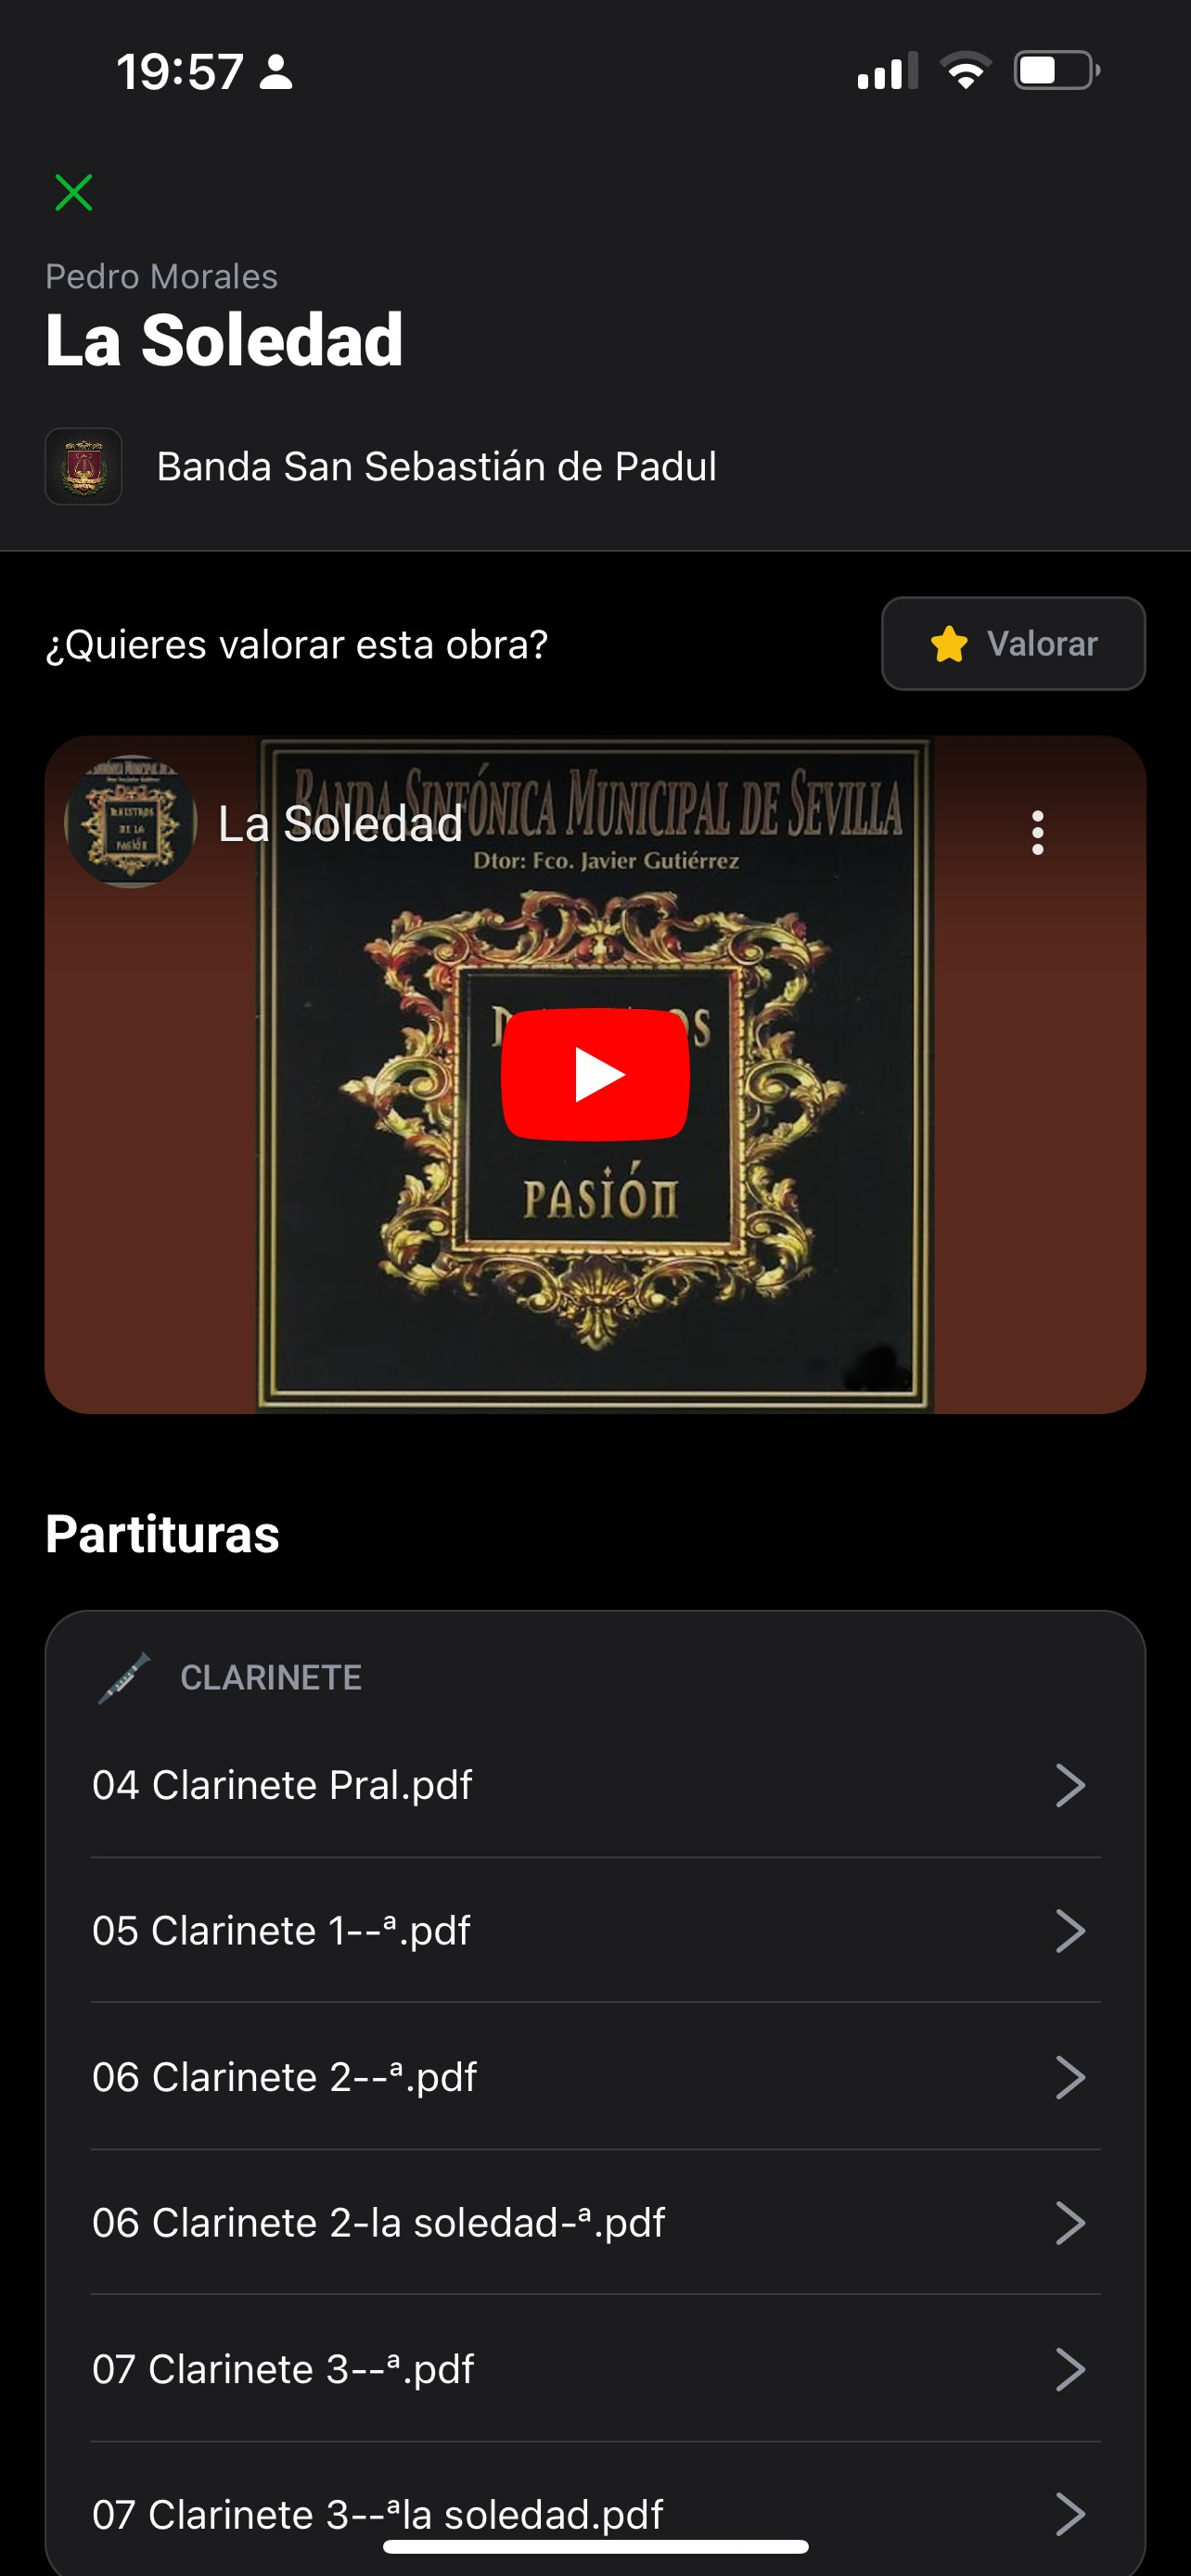
\includegraphics[width=\linewidth]{imagenes/capturas_glissandoo/IMG_0930.jpeg}
\endminipage
\caption{Capturas de la aplicación \textit{Glissandoo}}\label{fig:capturas_glissandoo}
\centering
\end{figure}

Algunas ventajas de esta alternativa son:

\begin{itemize}
    \item Presenta un diseño intuitivo y fácil de usar para todos los usuarios.
    \item Está disponible para las plataformas móviles iOS y Android, ampliamente usadas por los usuarios.
    \item Es gratuita si la agrupación tiene menos de 20 músicos.
    \item Es elaborada en por una empresa valenciana, lo cual da seguridad de que se adaptará a las necesidades de las agrupaciones musicales españolas.
    \item Incorpora un módulo de comunicaciones para poder centralizar todos los procesos de la agrupación en la aplicación, sin dejar los comunicados en otra aplicación de mensajería como WhatsApp.
\end{itemize}

Sin embargo, esta herramienta tiene varias desventajas:

\begin{itemize}
    \item El código es privado, y una agrupación no puede montar su propio servidor con la aplicación en cuestión.
    \item Es de pago para uso en agrupaciones con más de 20 miembros.
    \item Solo se puede usar en móvil, ya que no dispone de versión web ni de escritorio. (Esto ha cambiado durante la realización de este trabajo, ya que han implementado una versión web)
    \item Sigue existiendo duplicidad, ya que aunque los miembros usen esta aplicación, la comunicación bidireccional ocasional entre administradores y miembros de la banda se sigue realizando a través de una herramienta distinta de comunicación no especializada.
\end{itemize}

\subsection{Agregación de servicios no especializados}

Mediante \textit{agregación de servicios no especializados} nos referimos al uso de varias herramientas que no están especializadas para este caso de uso, pero que de cierta forma pueden suplir las necesidades:

\begin{itemize}
    \item Como almacenamiento de partituras, existen servicios como Google Drive, Dropbox o Microsoft OneDrive.
    \item Para la planificación de eventos y conciertos se puede usar un calendario web como Google Calendar o Microsoft Outlook.
    \item Para estimar la asistencia se pueden usar herramientas que permiten encuestas de este tipo como Doodle.
    \item Para controlar la asistencia real se puede usar una hoja de cálculo o herramientas como Alexia.
    \item Como medio de comunicación se utiliza otro servicio como WhatsApp o Telegram.
\end{itemize}

La ventaja de esta aproximación (la mayormente utilizada en la actualidad) es el mayor grado de personalización, ya que los servicios se pueden intercambiar si la funcionalidad o confiabilidad no es la esperada.

No obstante, las desventajas son numerosas, como ya se ha comentado anteriormente:
\begin{itemize}
    \item Gran carga de trabajo para los administradores.
    \item Redundancia de comunicaciones entre los miembros y los administradores.
    \item Muchas de estas herramientas requieren de suscripción premium para usar toda la funcionalidad.
\end{itemize}

%
\chapter{Mordente}

\section{Desarrollo de Mordente}


\section{Personas ficticias}


\section{Malla receptora de información}


\section{Descripción de la propuesta}




%
\chapter{Diseño de la interfaz de usuario}\label{chapter:diu}

A nivel de diseño de la interfaz, lo principal es reseñar que nos encontramos con una gran limitación: no podemos desarrollar una interfaz totalmente a nuestro gusto\footnote{El 16 de abril de 2022, la API para bots Telegram fue actualizada\cite{telegramWebappUpdate} con una nueva función para abrir una aplicación web sin salir del bot como respuesta a varios eventos. Sin embargo, esa opción se ha descartado para este trabajo ya que la implementación del bot se encontraba en estado avanzado y se ha analizado que las complicaciones técnicas de implementar esta nueva interfaz extenderían el tiempo de desarrollo considerablemente. Se propone como mejora futura.}, sino que debemos usar la API que nos proporciona Telegram.

Es decir, \textbf{Mordente bot} va a operar dentro de un chat, y como todo chat, la interfaz estará compuesto sola y únicamente por mensajes, que podrán ser de distinto tipo (texto, imágenes, documentos, stickers...). La única adición que aporta Telegram a esta interfaz es que los mensajes que envía el bot pueden adjuntar un menú de opciones que el usuario puede pulsar para pedir al bot una determinada acción, además de tener un menú de comandos disponible continuamente junto al cuadro de introducción de texto.

Esta rigidez de la interfaz puede ser vista de manera positiva, ya que aporta las siguientes ventajas:

\begin{itemize}
    \item Las decisiones de diseño son mucho más simples, puesto que no tenemos todo un elenco de estilos, formatos e interacciones que elegir. Por ejemplo, si el usuario quiere acceder a la información general sobre la aplicación, la mejor solución dentro del bot es que el usuario use un comando \texttt{/about} al cual el bot responde con un texto explicativo. En el caso de una aplicación web, la interacción por parte del usuario podría ser desde pulsar un botón hasta usar un atajo de teclado, y la visualización podría ser desde sobreponer un cuadro con la información hasta enlazar a una página distinta.
    \item La personalización ya está implementada para nosotros: esta característica se delega a la propia aplicación de Telegram, que permite seleccionar el tema claro u oscuro o cambiar el tamaño del texto.
    \item La accesibilidad está garantizada, ya que la interfaz de mensajes ya está totalmente adaptada a personas con discapacidad auditiva o visual.
    \item La familiarización del usuario con la interfaz es mayor de antemano, ya que con toda probabilidad habrá usado un chat antes y la interfaz del bot no es más que una extensión de un chat corriente. Esto le supondrá una adaptación más sencilla y más centrada en saber cuál es la funcionalidad que en cómo está dispuesta.
    \item El usuario interacciona de forma privada en un chat con el bot, de modo que el tono de respuesta del bot y el intercambio de mensajes hacen que el usuario perciba la interfaz como más amigable y cercana.
    \item Los entornos que más necesitan la comunicación se benefician de esta integración. Por ejemplo, en el caso que nos ocupa siempre se suele usar un grupo de mensajería, y un bot puede ser integrado en un grupo de Telegram.
\end{itemize}

Decimos que la limitación es autoimpuesta porque es tarea de este trabajo también analizar si las ventajas expuestas superan o igualan a las desventajas de operar dentro de un chat, es decir, si un bot de Telegram de este tipo puede operar sin la ayuda de una aplicación web o móvil que la acompañe. Dicho de otra forma, se pretende aprovechar esta oportunidad para analizar las interacciones humano-chat como parte de los objetivos de este trabajo.


\subsection{Bocetos de interfaz}

Con todo lo anterior en mente, pasamos a crear varios bocetos de lo que debería ser la interfaz entre el usuario y el bot: uno para listar elementos, un segundo para mostrar el detalle de un elemento y un tercero para crear un elemento nuevo.

\subsubsection{Lista de elementos}

Aunque se ha expuesto que la interfaz está limitada a la API disponible, en el caso de las listas tenemos 3 opciones si queremos que el usuario pueda acceder al detalle de cada elemento:
\begin{enumerate}
    \item Enviar un mensaje muy corto acompañado de un menú, cada botón del menú muestra el título de un elemento y al pulsar en él se recibe el detalle.
    \item Igual que la opción 1, pero añadiendo en el texto una lista de los elementos con un resumen de cada uno.
    \item Nueva opción explorada en este trabajo como variación de la opción 2: omitir el menú para no repetir los nombres, y en su lugar acompañar cada elemento de la lista con un comando del estilo \texttt{/event\_N} de manera que al pulsar y enviar el comando el bot responda con el detalle del elemento.
\end{enumerate}

En todo caso la lista debe ir acompañada de un botón para añadir elementos.

El diseño se ve en la figura \ref{fig:disenyo_lista}.

\begin{figure}[h]
\centering
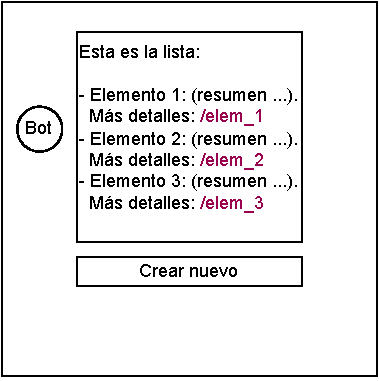
\includegraphics[width=0.5\textwidth]{imagenes/disenyo_interfaz/lista.drawio.pdf}
\caption{Diseño de la interfaz de lista}
\label{fig:disenyo_lista}
\end{figure}

\subsubsection{Detalle de elemento}

En este caso, toda la información sobre el elemento se muestra en el mensaje de respuesta, que va acompañado de un menú con las acciones que se pueden realizar con el elemento. Ver figura \ref{fig:disenyo_detalle}.

\begin{figure}[h]
\centering
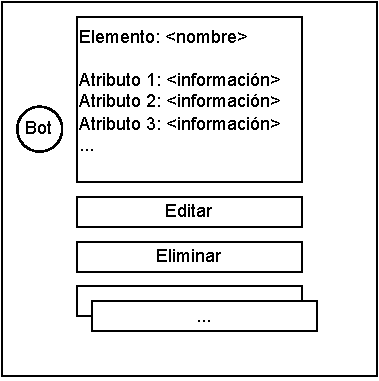
\includegraphics[width=0.5\textwidth]{imagenes/disenyo_interfaz/detalle.drawio.pdf}
\caption{Diseño de la interfaz del detalle de un elemento}
\label{fig:disenyo_detalle}
\end{figure}

\subsubsection{Creación de elemento}

La interfaz más sencilla y equivalente a un formulario para crear un elemento es una conversación: el bot va preguntando cada campo requerido al usuario, que puede saltar los campos opcionales mediante un botón de ``Saltar''.
Idealmente, para la introducción de fechas se debería mostrar un menú con forma de calendario. Ver figura \ref{fig:disenyo_creacion}.

\begin{figure}[h]
\centering
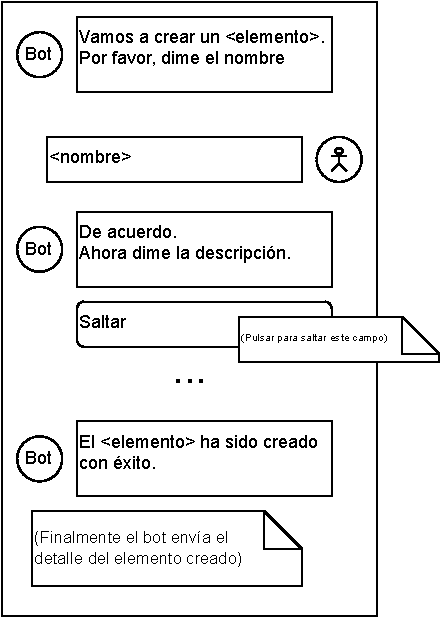
\includegraphics[width=0.5\textwidth]{imagenes/disenyo_interfaz/creacion.drawio.pdf}
\caption{Diseño de la interfaz de creación de un elemento}
\label{fig:disenyo_creacion}
\end{figure}

\section{Imagen de marca}

Para que la marca \textbf{Mordente} sea reconocible por los usuarios ya activos y los potenciales usuarios, vamos a definir tres elementos básicos: tipografía, logotipo y paleta de colores.

\subsection{Tipografía}

Para el logotipo hemos escogido la tipografía \textbf{Eczar} debido a su parecido con la mayoría de tipografías utilizadas para la edición de partituras.

El resto de la aplicación utilizará la tipografía por defecto del sistema, ya que esto es controlado por \textbf{Telegram}. La \textit{landing page} reproducirá este mismo comportamiento, de modo que todo el contenido excepto el logotipo utilizará la tipografía del sistema.

\subsection{Logotipo}

El logotipo usará un color \textbf{negro piano} (\#000000) con símbolo blanco.

Se compondrá del texto \textbf{mordente} en la tipografía escogida y un símbolo de mordente a la izquierda sobre el texto, ligeramente sobresaliendo por la izquierda del espacio que ocupa el texto.

Podemos ver el imagotipo (compuesto por el símbolo y el texto) en la figura \ref{fig:imagotipo}. El isotipo, compuesto solo por el símbolo y usado cuando se dispone de menos espacio, se puede ver en la figura \ref{fig:isotipo}.

\begin{figure}[]
\minipage{0.5\textwidth}
  \centering
  
\includegraphics[width=0.7\linewidth]{imagenes/logo_mordente.pdf}
  \caption{Imagotipo de \textbf{Mordente}}\label{fig:imagotipo}
\endminipage\hfill
\minipage{0.5\textwidth}%
  \centering
  
\includegraphics[width=0.7\linewidth]{imagenes/isotipo_mordente.pdf}
  \caption{Isotipo de \textbf{Mordente}}\label{fig:isotipo}
\endminipage
\end{figure}

\subsection{Paleta de colores}

Crearemos una paleta de colores usando la herramienta \texttt{coolors.co} (\url{https://coolors.co}) que nos permite encontrar colores complementarios fácilmente.

Tras decidir entre varias alternativas, la paleta generada se puede observar en la figura \ref{fig:paletaMordente}.

Por un lado tendremos los dos colores del logotipo: negro piano y blanco puro, a los que añadiremos el rojo ``Rubí Antiguo'' como color primario y el color naranja ``Mandarina'' como color secundario:

\begin{itemize}
    \item El \textbf{rojo ``Rubí Antiguo''} (\#832232) imita al color de la madera los instrumentos de cuerda frotada.
    \item El \textbf{naranja ``Mandarina''} (\#EF8354) complementa al color primario añadiendo más cantidad de amarillo.
\end{itemize}



\begin{figure}[h]
\centering
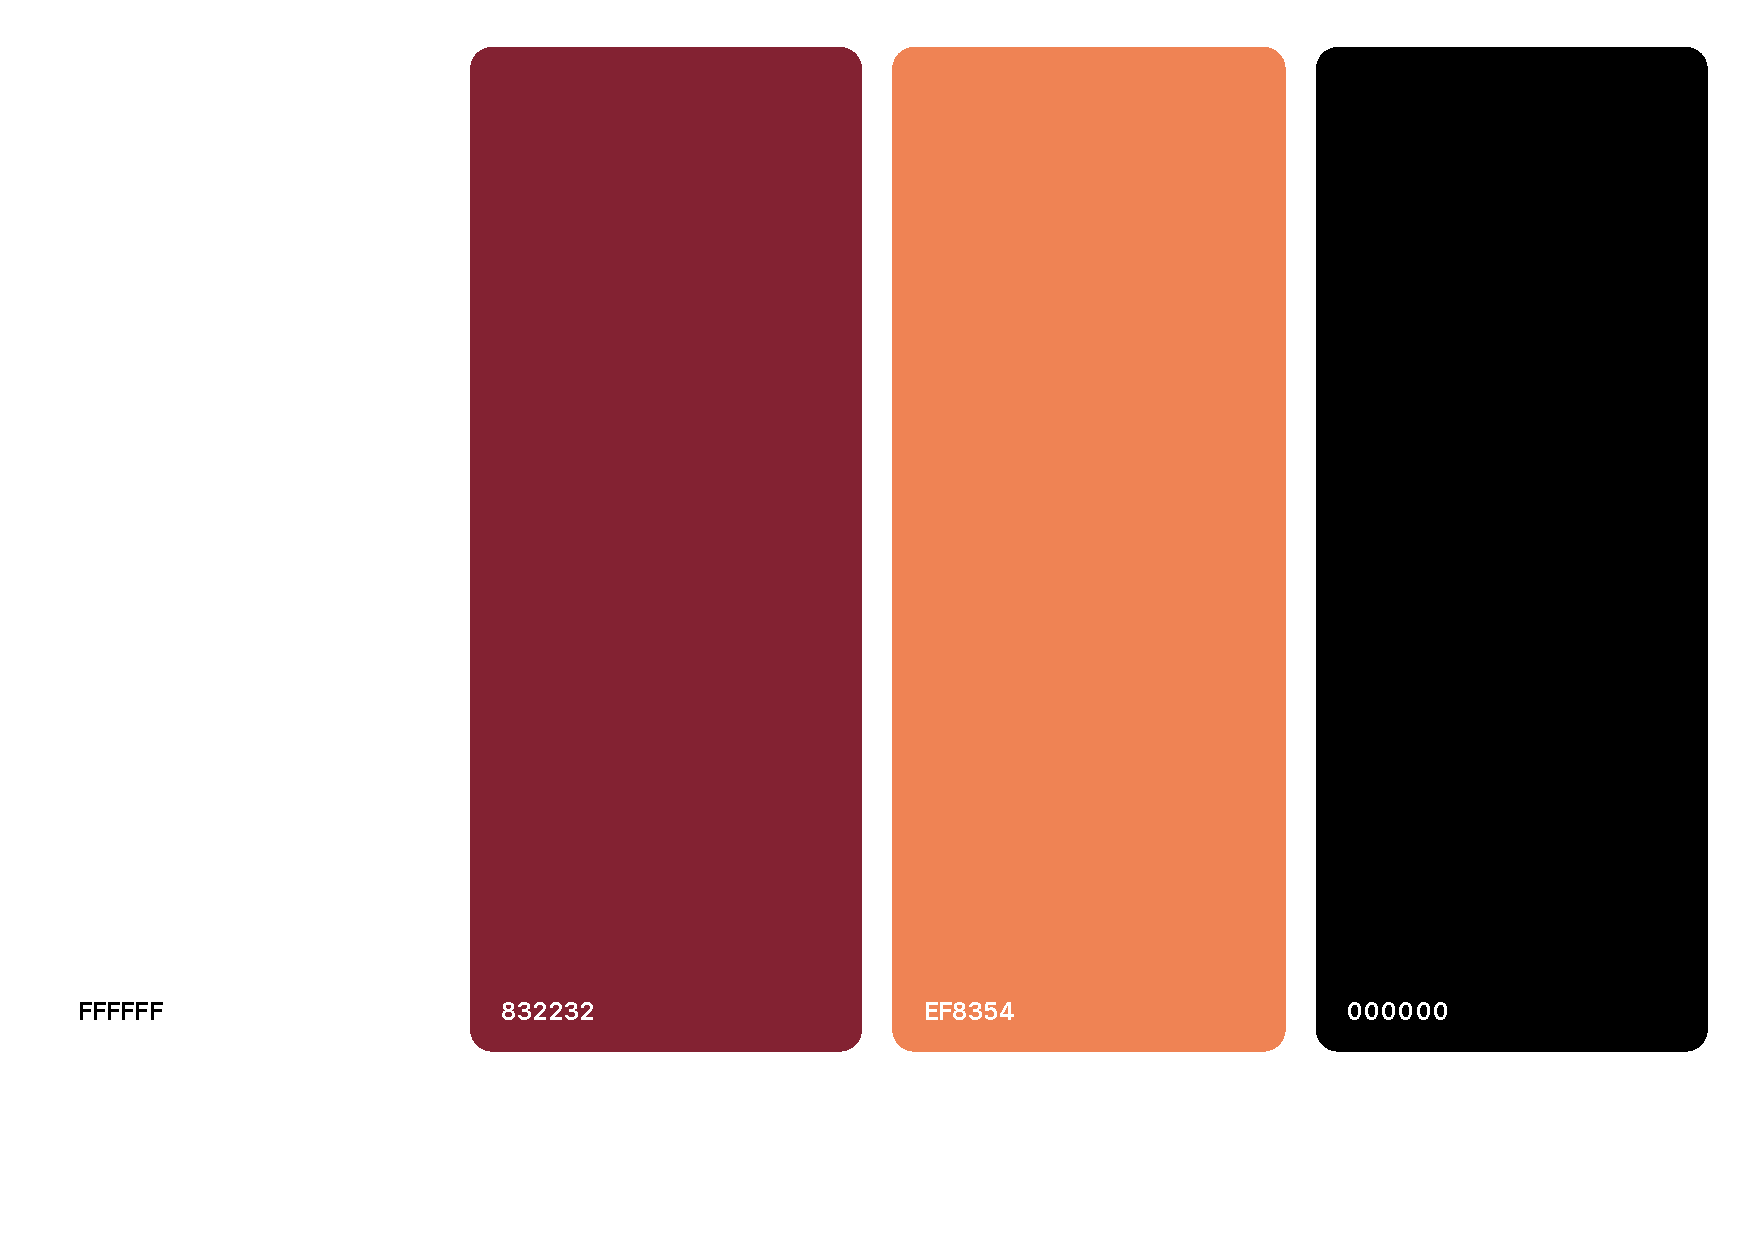
\includegraphics[width=\textwidth]{imagenes/disenyo_interfaz/mordente_paleta.pdf}
\caption{Paleta de colores}
\label{fig:paletaMordente}
\end{figure}

%
\chapter{Diseño técnico}

\section{Listado de historias de usuario (Backlog)}

\section{Historias de usuario}

\section{Modelo de la base de datos}

\section{Arquitectura de Mordente}

%
\chapter{Implementación}

En esta sección vamos a ahondar en ciertos detalles sobre \textbf{cómo se ha construido} este proyecto.

Las secciones están ordenadas de forma cronológica y a modo de relato, de forma que empezaremos explorando las funcionalidades que podemos aprovechar de las herramientas a usar y terminaremos creando la página web de promoción cuando la aplicación ya esté funcionando.


% Más subsecciones dependiendo de la metodología empleada


% Debe ser la sección más larga del documento.
% Usar herramientas de Ingeniería: diagramas, esquemas, plantillas, etc.

% - Incluir un diagrama de la arquitectura del sistema (visión general).
% - Indicar qué herramientas de la sección anterior se eligen para el
% desarrollo, por qué y para qué.
% - Poner solo pequeños trozos de código si es necesario para explicar
% detalles de implementación o justificar decisiones del diseño o de la
% tecnología.

\section{Exploración de funcionalidades}
% https://github.com/daniharo/mi-banda-bot

Comenzaremos la implementación del bot con un pequeño bot de prueba que nos permita descubrir cuál será el flujo de trabajo con las herramientas de programación que hemos escogido en la sección \ref{section:metodologias}. Estos son los pasos que daremos con este primer bot:

\begin{enumerate}
    \item Responder de manera básica básica a los mensajes recibidos, con un \texttt{!`Hola! Mensaje recibido.}
    \item Conectarse a una base de datos sencilla de una sola tabla, que guarda palabras.
    \item Listar palabras y eliminar palabras en la base de datos de forma global.
    \item Asignar las palabras a usuarios concretos para que solo puedan ver y eliminar las suyas.
\end{enumerate}

\subsection{Infraestructura de contenedores}
% docker, docker-compose

Para comenzar a desarrollar, primero crearemos los archivos que configuren los contenedores de \texttt{Docker}. Estos archivos nos permitirán levantar el bot en cualquier dispositivo fácilmente, solo ejecutando el comando \path{docker compose up}. Tal y como hemos explicado en la sección \ref{subsection:arquitecturaServicios}, en el entorno de desarrollo tendremos solo dos contenedores:

\begin{itemize}
    \item El contenedor \texttt{app} será el encargado de ejecutar el bot en \texttt{Node.js}. 
    \item El contenedor \texttt{postgres} contendrá la base de datos de \texttt{PostgreSQL}. Haremos que este contenedor exponga el puerto 5432 al sistema para poder depurar la base de datos.
\end{itemize}

Tendremos que añadir también dos volúmenes\footnote{\url{https://docs.docker.com/storage/volumes/}}:

\begin{itemize}
    \item Uno que hará que el código que estamos desarrollando se encuentre actualice en tiempo real dentro del contenedor sin tener que reconstruir la imagen.
    \item El otro estará asociado a la base de datos de forma que los datos guardados se almacenen de forma persistente.
\end{itemize}

El archivo \texttt{docker-compose.yml} resultante con contenedores y volúmenes se puede consultar en GitHub\footnote{\url{https://github.com/daniharo/mi-banda-bot/blob/98a0662b/docker-compose.yml}}.

\subsection{Conexión a base de datos}

El \textbf{ORM} (\textit{Object--relational mapper}) \texttt{prisma} nos ayudará a conectar con la base de datos de manera segura y aprovechando las ventajas del tipado estático que proporciona \textbf{TypeScript}: convierte los registros de la base de datos en objetos del lenguaje de programación que estamos usando y viceversa.

La configuración de \texttt{prisma} se realiza a través del esquema de la base de datos en el archivo \texttt{schema.prisma}\footnote{\url{https://github.com/daniharo/mi-banda-bot/blob/main/prisma/schema.prisma}}. El esquema se define en un lenguaje propio en un nivel de abstracción superior sobre SQL y que permite usar el mismo modelo intercambiando diferentes proveedores (PostgreSQL, MySQL o incluso proveedores No-SQL como MongoDB).

En esta primera parte, el esquema solo contendrá una tabla \texttt{Word}, de modo que en \texttt{schema.prisma} solo tendremos que configurar esa tabla, indicar que el proveedor es \texttt{PostgreSQL} y la URL de conexión\footnote{Archivo \texttt{schema.prisma}: \url{https://github.com/daniharo/mi-banda-bot/blob/main/prisma/schema.prisma}}.

Ejecutando el siguiente comando, \texttt{prisma} crea el código necesario para hacer todas las consultas a la base de datos, es decir, el \textbf{Cliente Prisma}:

\begin{verbatim}
prisma generate
\end{verbatim}

Ejecutaremos este comando cada vez que hagamos cambios en el esquema para generar un nuevo cliente.

Para usarlo desde \textbf{TypeScript}, solo necesitamos crear un archivo \\ \texttt{PrismaClient.ts} con el siguiente código:

\begin{verbatim}
import { PrismaClient } from "@prisma/client";

const prisma = new PrismaClient();

export default prisma;
\end{verbatim}

El objeto \texttt{prisma} contiene una clave para cada tabla de la base de datos, de manera que las consultas a la base de datos serían tan sencillas como:

\begin{verbatim}
// Consultar todas las palabras:
const words = await prisma.word.findAll();

// Eliminar palabras que contengan "palabra":
const deletedWord = await prisma.word.deleteMany({
  where: { word: { contains: "palabra" } }
});

// Modificar todas las palabras que comienzan por "foo":
const updatedWord = await prisma.word.updateMany({
  where: { word: { startsWith: "foo" } },
  data: { word: "nuevaPalabra" }
});
\end{verbatim}

La mayor ventaja que tenemos es que \texttt{prisma} es totalmente \textit{type-safe}: se obtiene un error directamente en el editor de código ante cualquier operación inválida. Por ejemplo, si intentamos crear un registro sin añadir un campo obligatorio, veremos esa línea subrayada de color rojo y \textbf{TypeScript} nos pedirá solucionarlo antes de poder ejecutar el programa.

\subsection{Manejo de mensajes de Telegram}

La lógica que nos permite implelmentar \texttt{grammY}, la biblioteca que hemos escogido en la sección \ref{subsection:elegirFramework} para comunicarnos con la API de Telegram, es la siguiente:

\begin{itemize}
    \item Cada mensaje entrante pasa por una cadena de funciones llamadas \textbf{middleware}. A cada \textbf{middleware} le podemos dar una responsabilidad distinta:
    \begin{itemize}
        \item \textbf{Modificar} el objeto \texttt{ctx} que va recorriendo todos los \texttt{middleware} y que contiene toda la información del mensaje entrante para añadir información adicional. En este caso, debe llamar a \texttt{next()} para que el mensaje siga recorriendo el resto de \texttt{middleware}.
        \item \textbf{Manejar} el mensaje respondiendo, actualizando la base de datos, o con cualquier tarea que se necesite. En este caso no se llama a \texttt{next()} ya que el recorrido del mensaje terminaría ahí.
    \end{itemize}
    \item El \texttt{middleware} se instala en el bot mediante métodos como \texttt{.use}, \texttt{.on} o \texttt{.command}:
    \begin{itemize}
        \item \texttt{.use} nos permite instalar \texttt{middleware} que se ejecuta siempre.
        \item \texttt{.on} nos permite usar filtros sencillos como \texttt{.on("message")}, en este caso para que ese \texttt{middleware} solo maneje mensajes y no otros eventos como pulsaciones en menús.
        \item \texttt{.command} maneja mensajes que incluyan el comando especificado como primer argumento. Por ejemplo, \texttt{.command(``/about'')} se encargaría de responder al comando \texttt{/about}.
    \end{itemize}
\end{itemize}

Para esta primera prueba, vamos a instalar solo estas funciones de \\ \texttt{middleware}:

\begin{itemize}
    \item \texttt{.command(``start'')} responderá al inicio del bot con un \texttt{``Hey!''}.
    \item \texttt{.command(``list'')} responderá con la lista actual de palabras.
    \item \texttt{.command(``add'')} añadirá la palabra especificada en el mensaje.
    \item \texttt{.command(``delete'')} eliminará la palabra que se concrete.
    \item \texttt{.on(``message'')} estará al final y responderá a todos los mensajes que no sean manejados por el \texttt{middleware} anterior con un \texttt{``Lo siento, no sé de qué me hablas''}.
\end{itemize}

El código de este primer bot de prueba está disponible en GitHub\footnote{\url{https://github.com/daniharo/mi-banda-bot/blob/main/src/app.ts}}.

\section{Internacionalización}

Si la aplicación crece, es probable que la terminen usando usuarios que hablan otro idioma, ya sea otra lengua cooficial de nuestro país (como el catalán o el gallego) o una lengua foránea.

Vamos a dejar el código preparado para que, si esto ocurre, solo tengamos que añadir las traducciones para el idioma correspondiente.

Para ello, añadimos el paquete \path{@grammyjs/fluent}\footnote{\url{https://www.npmjs.com/package/@grammyjs/fluent}}. Este paquete nos permitirá usar la sintaxis del \textbf{Proyecto Fluent}\footnote{\url{https://projectfluent.org/}} de \textbf{Mozilla} para crear las traducciones. Para añadirlo, solo tenemos que ejecutar siguiente comando, el mismo que utilizaremos con todas las dependencias que añadamos:

\begin{verbatim}
yarn add @grammyjs/fluent
\end{verbatim}

Incluiremos en el archivo \path{src/locales/es.ftl}\footnote{\url{https://github.com/daniharo/mordente/blob/main/src/locales/es.ftl}} las cadenas de texto que necesitemos usar en el bot.

Para agilizar el desarrollo, dejaremos en línea dentro del código las cadenas de texto cortas y que no ocupen más de una línea. Convertir estas cadenas en traducciones es una tarea mecánica que se puede posponer al momento en el que tengamos un prototipo funcional con el que hacer las pruebas de usabilidad.

\section{Separación MVC: Plantillas}

El patrón arquitectónico \textbf{Modelo-Vista-Controlador} se usa comúnmente para desarrollar interfaces de usuario dividiendo la lógica en tres elementos conectados\cite{whatIsMVC}. Esto permite hacer una mejor \textbf{división del código}.

Dado que no existe ningún \textit{framework opinionado}\footnote{Con \textit{opinionado} nos referimos a aquel marco de trabajo en el que se manifiestan claramente qué técnicas y procesos se deben seguir para su uso: su documentación especifica \textbf{cómo} proceder y no solo \textbf{qué} se puede hacer.} para desarrollar bots de Telegram que siga este patrón (sí existen para desarrollo web, por ejemplo \textbf{Symphony}\footnote{\url{https://symfony.com/}} para PHP), vamos a estructurar el código de la siguiente forma:

\begin{itemize}
    \item \textbf{Modelo:} En la ruta \path{src/models/} implementaremos toda la comunicación directa con al base de datos: consultas, eliminaciones y modificaciones, en un archivo distinto para cada modelo.
    \item \textbf{Vista:} Las vistas estarán compuestas por:
    \begin{itemize}
        \item \textbf{Menús} en línea que aparecen debajo de un mensaje enviado por el bot, se encontrarán en la ruta \path{src/menus/}.
        \item \textbf{Conversaciones} que mantiene el bot con un usuario, en la ruta \path{src/conversations/}.
        \item \textbf{Plantillas} complejas de mensajes que debe enviar el bot sustituyendo ciertas variables o recorriendo un vector de elementos. Usaremoe el motor de plantillas \texttt{Pug.js}\footnote{\url{https://pugjs.org/api/getting-started.html}} y guardaremos las plantillas en la ruta \path{src/templates/}.
    \end{itemize}
    \item \textbf{Controlador:} Los manejadores de mensajes serán las funciones que actúen de controlador. Estos se pueden escribir a modo de \texttt{Composer} o de \texttt{Middleware}, por lo que tendremos las carpetas \path{/src/composers/} y \path{/src/middleware/}. El archivo \path{app.ts} se encargará de iniciar la cadena de llamadas a todos los controladores.
\end{itemize}

En la figura \ref{fig:mvc} se representa visualmente la separación de responsabilidades.

\begin{figure}[h]
\centering
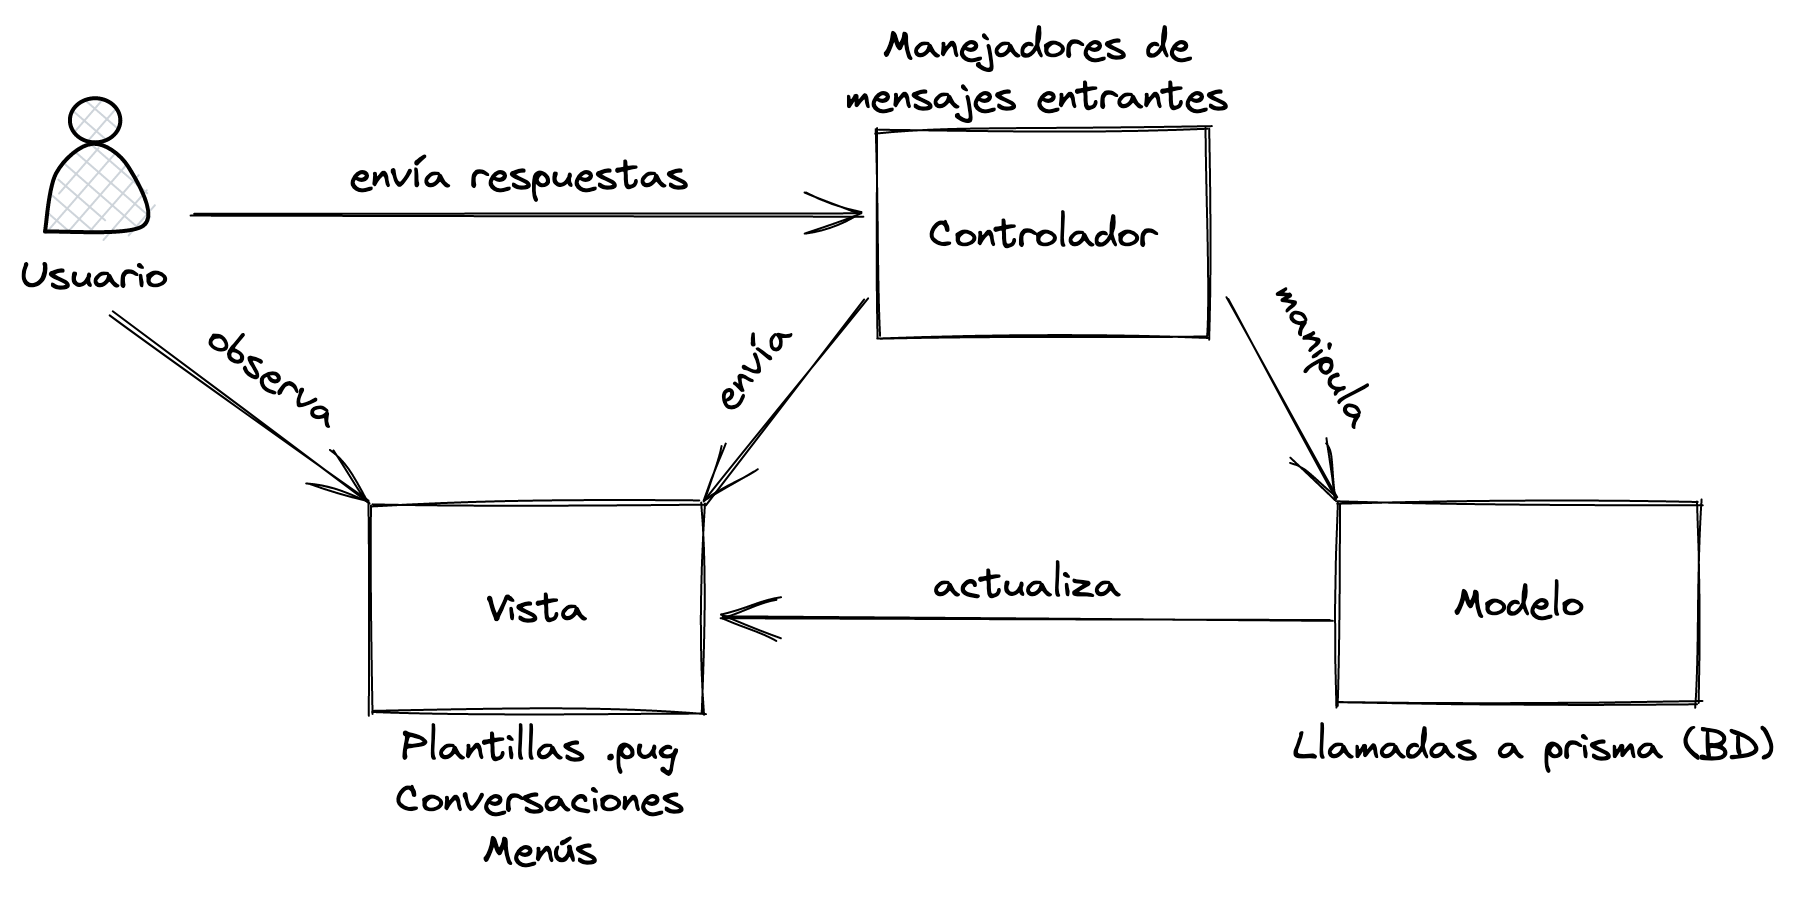
\includegraphics[width=\textwidth]{imagenes/implementacion/mvc.png}
\caption{Separación Modelo-Vista-Controlador}
\label{fig:mvc}
\end{figure}

Hasta ahora tenemos todos los elementos que se han explicado, excepto las plantillas. Tras instalar el motor de plantillas con \path{yarn add pug}, deberemos asegurarnos de que las plantillas se compilan cuando se inicia el bot\footnote{\textit{Commit:} \url{https://github.com/daniharo/mordente/commit/107f7e50}}.

\section{Unirse a un grupo}

Cuando el bot se inicia, presentará a los usuarios dos opciones rápidas: crear una nueva agrupación o unirse a una ya existente.

Dado que la creación de la agrupación requiere iniciar una conversación con el usuario, implementaremos primero la funcionalidad de unirse, que solo requerirá de un comando \texttt{/start} por parte del usuario acompañado de un código de invitación, que de momento será el ID de la agrupación.

Para implementar esta funcionalidad, vamos a usar un truco: por ahora crearemos las agrupaciones en la base de datos de forma manual, mediante la interfaz que nos proporciona \texttt{prisma studio}\footnote{\url{https://www.prisma.io/studio}}.

Añadimos por tanto el menú \texttt{startMenu} que da la bienvenida a los usuarios y une al usuario a una agrupación si el comando viene acompañado de un código\footnote{\textit{Commit:} \url{https://github.com/daniharo/mordente/commit/5ded357c}}. Esto es posible gracias a la característica \textbf{Deep Linking}\footnote{\url{https://core.telegram.org/bots/features\#deep-linking}} de la \textbf{API para Bots de Telegram}.


\section{Crear, mostrar y eliminar agrupaciones}
Todas las funcionalidades del bot dependen del hecho de que existan agrupaciones creadas en la base de datos por administradores, a las cuales se podrán unir los miembros.

Por ello esta será la próxima tanda de historias de usuario a implementar.

Permitiremos crear una agrupación utilizando el comando \texttt{/create}\footnote{\textit{Commit:} \url{https://github.com/daniharo/mordente/commit/82fa3897}} o desde el menú de inicio del bot, que se obtiene con el comando \texttt{/start}\footnote{\textit{Commit:} \url{https://github.com/daniharo/mordente/commit/8cfd020f}}.

Además, añadimos la vista (plantilla) necesaria para ver el detalle de una agrupación, \texttt{ensemble-detail.pug}\footnote{\textit{Commit:} \url{https://github.com/daniharo/mordente/commit/b65de583}}. Permitiremos también al usuario cancelar la conversación para crear la agrupación en cualquier momento, mediante un comando \texttt{/cancel}\footnote{\textit{Commit:} \url{https://github.com/daniharo/mordente/commit/90ddedfb}}.


\section{Optimización de la autenticación en cada mensaje}\label{section:useAccount}
% https://github.com/daniharo/mordente/compare/be269acf...331168c6

En la práctica totalidad de los mensajes que recibe el bot necesitamos comprobar cuál es el ID de ese usuario en nuestra base de datos. Esto es así porque, en vistas a futuro, hemos decidido que el ID del usuario en Telegram no sea el ID del usuario en nuestra base de datos, de manera que nuestra aplicación no dependa totalmente de Telegram.

Hacer una consulta a la base de datos en todas las funciones que manejan mensajes es repetitivo e ineficiente, por lo que se ha decidido implementar un \textit{middleware} encargado de:

\begin{itemize}
    \item Consultar si tenemos el ID de ese usuario en la sesión\footnote{\url{https://grammy.dev/plugins/session.html}} actual.
    \item Si no lo tenemos, comprobar si existe en la base de datos.
    \begin{itemize}
        \item Si existe en la base de datos pero hace demasiado tiempo de la última actualizacion de nuestra base de datos, actualizamos y guardamos el ID en la sesión.
        \item Si existe en la base de datos y está actualizado, solo guardamos el ID en la sesión.
        \item Si no existe en la base de datos, lo añadimos (creamos una cuenta) guardando el ID obtenido en la sesión.
    \end{itemize}
    \item Finalmente, ejecutamos \texttt{ctx.userId = ctx.session.userId} para que todos los manejadores de mensajes puedan acceder al ID fácilmente.
\end{itemize}


Una vez está implementado, eliminamos todas las consultas a la base de datos en el código para sustituirlas por \texttt{ctx.userId}\footnote{\textit{Commits:} \url{https://github.com/daniharo/mordente/compare/be269acf...331168c6}}.

\section{Crear, mostrar y eliminar eventos}

Una de las funcionalidades más centrales de este proyecto es la de gestionar \textbf{eventos}.

Teniendo la funcionalidad de crear, ver y eliminar agrupaciones implementada, la funcionalidad relacionada con los eventos solo requiere adaptar el código anterior a las características de los eventos. Necesitaremos una conversación para crear los eventos (\texttt{createEventConversation}\footnote{\textit{Commit:} \url{https://github.com/daniharo/mordente/commit/65979e02}}), las plantillas correspondientes al detalle del evento (\texttt{event-detail.pug}) y a la lista de eventos (\texttt{events-summary.pug}) y los menús para la lista de eventos (\texttt{eventListMenu}) y el detalle de evento (\texttt{eventMenu})\footnote{\textit{Commits:} \url{https://github.com/daniharo/mordente/compare/77b0fb44...d820211d}}.



\subsection{Selector de fecha\footnote{Posteriormente durante el desarrollo del proyecto se ha detectado que este selector de fecha interfiería con una nueva versión de la dependencia \texttt{grammy-conversations}, la cual necesitábamos actualizar. Solucionar este problema en el selector de fecha demoraría demasiado el desarrollo, por lo que se ha optado por sustituirlo temporalmente por mensajes de texto del formato \texttt{DD/MM/YYYY} para la fecha y \texttt{HH:MM} para la hora.}}\label{subsection:selectorCalendario}

Dado que uno de los atributos de cada evento es la fecha y hora de inicio y la fecha y hora de fin, debemos otorgar al usuario la posibilidad de responder al bot fácilmente cuando se les pide estos datos.

Una forma muy intuitiva de introducir una fecha es proporcionar al usuario un calendario donde pulsar para seleccionarla.

Implementar un calendario dentro de Telegram presenta numerosas complicaciones técnicas, sin embargo hemos conseguido implementarlo y publicarlo para que el resto de la comunidad pueda mejorar este código y usarlo en sus proyectos\footnote{\url{https://www.npmjs.com/package/grammy-calendar}}.

En la URL \url{https://mordente.es/video/calendar.mp4} se puede ver un vídeo corto mostrando el funcionamiento de este calendario.

\subsection{Guardar sesión en la base de datos}\label{subsection:adaptadorPrisma}

% qué se guarda en la sesión: id de usuario, paso dentro de una conversación, etc

Uno de los problemas que hemos detectado durante la implementación de esta funcionalidad es que hasta ahora la \textbf{sesión del usuario} se está guardando en la memoria principal del sistema. La \textbf{sesión del usuario} guarda información como:

\begin{itemize}
    \item ID del usuario que nos ha enviado un mensaje, por la implementación de la sección \ref{section:useAccount}.
    \item Paso en el que se encuentra dentro de una conversación para crear o eliminar una agrupación, un evento...
    \item ID del elemento que se encuentra editando en un determinado momento.
\end{itemize}

En el caso de que se reinicie el bot momentáneamente, no queremos que el bot pierda todo el contexto que se encontraba manejando. Por ejemplo, mientras un usuario crea un evento, si ha llegado a la mitad de la conversación pero reiniciamos el bot, debe volver a empezar. Por esto, vamos a hacer uso de una de las posibilidades que nos ofrece \textbf{grammY}: guardar la sesión en la base de datos.

% contribución a grammY

El \textit{framework} \textbf{grammY} ofrece diversos \textbf{adaptadores} sesión-base de datos que permiten guardar la sesión en la base de datos de forma transparente para el desarrollador. Sin embargo, no hay ningún adaptador para el ORM que estamos utilizando, \texttt{prisma}, tal y como hemos encontrado en un \textit{issue} de GitHub\footnote{\url{https://github.com/grammyjs/storages/issues/80}}.

La solución pasa por contribuir a la comunidad del software libre con la implementación de este adaptador. Por ello, nos ponemos manos a la obra y, una vez el trabajo está hecho, hacemos la petición de integrar el adaptador en el repositorio de adaptadores\footnote{\textit{Pull Request:}  \url{https://github.com/grammyjs/storages/pull/108}}, no sin encontrar dificultades durante el proceso.

% problema: tests

Los mayores problemas en este paso han sido para hacer funcionar los tests, tal y como se puede ver en el \textit{Pull Request}, aunque finalmente hemos conseguido hacerlos funcionar.

Tras publicar el adaptador, el creador de \textbf{grammY} ha compartido con la comunidad un agradecimiento al autor de este proyecto por esta contribución\footnote{Mensaje en canal de Telegram: \url{https://t.me/grammyjs_news/35}}.

\section{Configuración del \textit{linter}}

% ESLint, ESLint-typescript

El motivo por el que estamos usando el lenguaje \textbf{TypeScript} en lugar de \textbf{JavaScript} en este proyecto es porque el \textbf{tipado estático} evita gran parte de los errores que se puedan dar al ejecutar el programa por despistes del programador, además de mejorar el autocompletado que proporciona el IDE.

Sin embargo, se puede dar un paso más en la dirección de evitar errores que se dan durante la ejecución: un \textit{linter} es un programa que ``revisa y observa el código en busca de errores que le puedan afectar''\cite{whatIsLinter}. Algunos de los errores que puede detectar son\cite{whatIsLinter}:

\begin{itemize}
    \item Código poco intuitivo o \textbf{difícil de mantener}.
    \item Uso de \textbf{malas prácticas}.
    \item \textbf{Estilos} de código \textbf{inconsistentes}.
\end{itemize}

Además, nos proporciona la posibilidad de solucionar automáticamente muchos de los errores que detecta.

El \textit{linter} más conocido para \textbf{JavaScript} y \textbf{TypeScript} es \textbf{ESLint}\footnote{\url{https://eslint.org/}}. Por ello hemos decidido configurar \textbf{ESLint} en el proyecto\footnote{Cambios en el código: \url{https://github.com/daniharo/mordente/compare/a1f07349...0e8f3aaa}} de manera que esté integrado con \textbf{TypeScript} y solucionar todos los problemas que nos ha detectado tras la configuración\footnote{\textit{Commit:} \url{https://github.com/daniharo/mordente/commit/100b60b2}}.

\section{Limitación de errores para el bot}\label{section:errorBoundary}
% https://github.com/daniharo/mordente/commit/0299185c

Hemos detectado que cuando el programa lanza una excepción en cualquier punto, la ejecución termina por lo que el bot deja completamente de funcionar.

El \textit{framework} usado para crear el bot, \textbf{grammY}, nos permite \textit{vallar} los errores, lo que se conoce como \textbf{error boundary}. Mediante esta técnica, podemos asignar para cada tipo de mensaje que le pueda llegar al bot qué queremos que pase cuando se lance una excepción

En nuestro caso aplicaremos esta técnica en el nivel más alto de la aplicación, de manera que todos los errores pasen por este manejador de errores. Solo tenemos que añadir el código\footnote{\textit{Commit:} \url{https://github.com/daniharo/mordente/commit/0299185c}}:

\begin{verbatim}
bot.catch(error => {
    // Qué queremos hacer con el error. 
    // En nuestro caso, mostraremos el mensaje de error
    // en la consola.
    ...
    console.error(`Error handling update ${update_id}:`);
    ...
})
\end{verbatim}


\section{Mejora del flujo de trabajo para depurar}
% node inspect (commit https://github.com/daniharo/mordente/commit/5a64a8516519d1f21e33a8810252bb9b79a3588b)

Durante el desarrollo, es muy frecuente encontrar problemas y errores cuyo origen resulta difícil de averiguar. Por ello habitualmente recurrimos a escribir una salida en la consola que indique el valor de ciertas variables cuando el bot recibe un mensaje. Sin embargo esta es una forma poco eficiente de depuración ya que nos proporciona información limitada.

\texttt{Node.js} proporciona una forma de depurar que expone en un puerto toda la información de la ejecución actual del programa para que, utilizando una herramienta externa (como IntelliJ\cite{debugIntelliJ} o Chrome\cite{debugChrome}), podamos depurar de forma eficiente la ejecución del programa.

Para ello, modificamos el archivo \path{docker-compose.yml} convenientemente para exponer el puerto \texttt{9200} al sistema y configuramos \texttt{node} para que registre la información de depuración en ese puerto\footnote{\textit{Commit:} \url{https://github.com/daniharo/mordente/commit/5a64a851}}.


\section{Respuestas de asistencia prevista}
% https://github.com/daniharo/mordente/commit/9d2059609cc696405f6f4cbd2b2590ff2878eb98

Una de las funcionalidades más interesantes de nuestro bot será la gestión de la asistencia prevista: los miembros avisan si podrán ir o no a los eventos y los administradores obtienen esta información.

Para ello, lo primero que haremos será permitir a los usuarios responder si asistirán o no a un evento, añadiendo los correspondientes botones al menú del detalle de un evento\footnote{\textit{Commit:} \url{https://github.com/daniharo/mordente/commit/9d205960}}.


\subsection{Pedir justificación}
% https://github.com/daniharo/mordente/commit/06efba49a35e562bf23756bc2fa2fdf8d150ca47

También es conveniente que los miembros opcionalmente puedan justificar su ausencia a un determinado evento, por lo cual si expresan que no asistirán, iniciaremos una conversación (\texttt{attendanceConversation}) para preguntar al miembro por qué no podrá asistir, acompañando la pregunta de un botón de \texttt{Saltar} dado que esta justificación será opcional\footnote{\textit{Commit:} \url{https://github.com/daniharo/mordente/commit/06efba49}}.

\subsection{Notificar administradores}
% https://github.com/daniharo/mordente/commit/fb7e33e4d485841c9d14a15acff932f66f270476

Los administradores deben ser notificados inmediatamente cuando un miembro responde sobre su asistencia.

Tan pronto como el bot reciba la respuesta de un miembro, se se comunicará con todos los administradores de la agrupación para informar de ello\footnote{\textit{Commit:} \url{https://github.com/daniharo/mordente/commit/fb7e33e4}}.

\section{Asignación de miembros a eventos}
% https://github.com/daniharo/mordente/commit/9e951c77ee1b2a68ad6096b7ebf269192ff75522

% https://github.com/daniharo/mordente/commit/77ad84b13aae9dba6c6f44f890fb200695459148
% https://github.com/daniharo/mordente/commit/b111f68ee919500346a61c1c3d711caed6fd9c17
Ahora haremos que los eventos puedan ser asignados a usuarios concretos.

Durante la creación de un evento, preguntaremos a un usuario si quiere asignarlo a todos los usuarios o si asignará manualmente más tarde\footnote{\textit{Commit:} \url{https://github.com/daniharo/mordente/commit/9e951c77}}. Haremos también que los usuarios solo puedan ver los eventos que tienen asignados\footnote{\textit{Commit:} \url{https://github.com/daniharo/mordente/commit/77ad84b1}}.

Por último, implementaremos un menú paginado que permita a los administradores elegir exactamente qué miembros estarán asignados a cada evento\footnote{\textit{Commit:} \url{https://github.com/daniharo/mordente/commit/b111f68e}}. Para la paginación guardaremos en la sesión del usuario en qué página se encuentra en cada momento.

\section{Recordatorio de eventos diarios}
% https://github.com/daniharo/mordente/commit/33859f0544f298262d72be75aac76bdbc1244d31

La historia de usuario relativa a los recordatorios diarios de eventos es la única que no dispara una petición al bot sino que dispara el bot por sí mismo cada cierto tiempo.

Es por ello que debemos configurar una tarea \texttt{cron} que se ejecute cada día para enviar los recordatorios. En esta tarea, se consultan a la base de datos los eventos que tienen lugar hoy y se envía un mensaje a cada usuario que tiene eventos hoy con la información de los eventos correspondientes\footnote{\textit{Commit:} \url{https://github.com/daniharo/mordente/commit/33859f05}}.




\section{Adición y eliminación de administradores}
% https://github.com/daniharo/mordente/commit/60db0538dcb3f31d9b67ad91915b13a3337088e3

Para añadir y eliminar administradores, ofereceremos a los ya administradores, en el menú de membresía de los demás usuarios, la opción \textbf{Hacer admin} o \textbf{Quitar de admin}.

Para ello implementamos las funciones correspondientes al modelo y los botones correspondientes en el menú reseñado\footnote{\textit{Commit:} \url{https://github.com/daniharo/mordente/commit/60db0538}}.




\section{Despliegue de producción}

Nos encontramos en un punto donde faltan muy pocas historias de usuario por implementar, por lo cual va siendo conveniente que el bot esté disponible de forma continua en un entorno de producción.

\subsection{Modificaciones previas en el código}

Antes de proceder a configurar un servidor de producción con nuestro código, es necesario modificar ciertas partes del código.

\subsubsection{PM2: evitando caídas}
% hablar de pm2 https://github.com/daniharo/mordente/commit/0783b132043fc3dc85ce73b547d9b9db8b21bae4

Aunque en la sección \ref{section:errorBoundary} hayamos implementado un método que capta los errores de forma que se responde al usuario con un error en lugar lanzar una excepción que pare la ejecución del bot, en el entorno producción será necesario dar un paso más.

\textbf{PM2}\footnote{\url{https://pm2.keymetrics.io/}} es un gestor de procesos para \texttt{Node.js} que, entre otras funcionalidades, permite configurar nuestro programa de \texttt{Node.js} como un demonio. De esta forma, si en algún momento el bot se cae por alguna excepción, se volverá a levantar automáticamente.

Es por ello que se ha decidido añadir \textbf{PM2} como dependencia e implementar su respectiva configuración\footnote{\textit{Commit:} \url{https://github.com/daniharo/mordente/commit/0783b132}}.

\subsubsection{Modificaciones en los contenedores de \texttt{docker}}
% nuevo docker compose https://github.com/daniharo/mordente/commit/8f5739ae9d013687f010600cbded7c3ec5d5dada

En el entorno de desarrollo, hay varios contenedores funcionando que tienen puertos TCP expuestos hacia el exterior:

\begin{itemize}
    \item La base de datos tiene expuesto el puerto \texttt{5432} para poder depurar en tiempo real la base de datos de manera gráfica con \path{prisma studio}\footnote{\url{https://www.prisma.io/studio}}.
    \item El bot expone el puerto \texttt{9200} para poder depurar la ejecución del bot\footnote{\url{https://nodejs.org/en/docs/guides/debugging-getting-started/}}.
\end{itemize}

En un entorno de producción queremos que los contenedores estén totalmente aislados. Para ello se han modificado los archivos \texttt{docker-compose}, de manera que ahora tenemos tres\footnote{\textit{Commit:} \url{https://github.com/daniharo/mordente/commit/8f5739ae}}:

\begin{itemize}
    \item \texttt{docker-compose.yml}: Es el archivo base que usarán todos los entornos.
    \item \texttt{docker-compose.override.yml}: Añade los puertos a exponer en el entorno de desarrollo.
    \item \texttt{docker-compose.prod.yml}: Configura el bot para el entorno de producción ajustando la variable de entorno \texttt{NODE\_ENV} a \texttt{"production"}.
\end{itemize}


\subsubsection{Migraciones de la base de datos}
% migración de base de datos manual ahora https://github.com/daniharo/mordente/commit/98f3186d251d2c4da88e101ed11c5155b763ddb0

Hasta ahora las migraciones de la base de datos\footnote{Las \textbf{migraciones} ajustan la base de datos a cambios en el esquema SQL.} se realizaban de forma automática cada vez que se encendía el bot con \path{docker compose up}.

A partir de ahora, querremos que las migraciones se apliquen de forma manual cuando se despliegue código a producción que incluya cambios en el esquema. Para ello, añadimos como \textit{scripts} los comandos necesarios para realizar las migraciones\footnote{\textit{Commit:} \url{https://github.com/daniharo/mordente/commit/98f3186d}}.


\subsubsection{Compilación del código TypeScript a JavaScript}
% compilar TS antes de iniciar https://github.com/daniharo/mordente/commit/3be387e6b5cf21ab101ed26b03c3d6e96892916c

El código que hemos escrito en el lenguaje \textbf{TypeScript} debe ser \textbf{transpilado}\footnote{Transpilar código fuente significa transformarlo desde un lenguaje de programación a otro con un nivel similar de abstracción\cite{whatIsTranspiler}.} al lenguaje \textbf{JavaScript} para que \texttt{Node.js} pueda leerlo.

Idealmente debemos efectuar esta transpilación mientras construimos la imagen de \texttt{docker}, mientras actualmente lo estamos haciendo al iniciar la ejecución del bot. Por ello realizaremos los cambios oportunos en el código para corregirlo\footnote{\textit{Commit:} \url{https://github.com/daniharo/mordente/commit/3be387e6}}.


\subsection{Creación de servidor virtual}

Ya tenemos el código listo para desplegarlo en un servidor de producción que esté encendido las 24 horas del día.

Tal y como hemos decidido durante el \textbf{Diseño Técnico} en la sección \ref{subsection:elegirCloud}, procedemos a crear un servidor virtual en la plataforma de \textbf{DigitalOcean}. Para ello empezamos registrándonos en su página web\footnote{\url{https://cloud.digitalocean.com}} y creando un nuevo proyecto llamado \texttt{mordente}.

Los pasos para crear el servidor han sido los siguientes:

\begin{enumerate}
    \item Pulsar \textbf{Create} y \textbf{Droplets}. Accederemos a la pantalla de creación de Droplets.
    \item Seleccionamos la pestaña \textbf{Marketplace}, donde podremos encontrar múltiples plantillas preconfiguradas para necesidades comunes.
    \item Buscamos \texttt{Docker} dentro del \textbf{Marketplace}, y seleccionamos el resultado principal.
    \item Ajustamos la configuración para usar el plan más económico y ubicar el servidor en Frankfurt, la región con menor latencia desde Granada.
    \item Añadimos la clave pública SSH de nuestro equipo para que la autenticación solo pueda realizarse mediante esta.
\end{enumerate}

Una vez tenemos el servidor creado, los pasos a ejecutar en el servidor para encender el bot son:

\begin{verbatim}
# Generar clave privada y pública
ssh-keygen

# Abrir la clave pública para añadirla en GitHub
# (https://github.com/settings/keys)
cat .ssh/id_ed25519.pub

# Crear carpeta para repositorios y abrirla
mkdir repos && cd repos

# Clonar el repositorio de GitHub
git clone git@github.com:daniharo/mordente.git

# Ejecutar el bot
docker compose -f docker-compose.yml -f docker-compose.prod.yml up

# Ejecutar las migraciones de la base de datos
docker compose exec app yarn run migrate:prod
\end{verbatim}

Tras ejecutar estos pasos, ya tenemos el bot funcionando en el entorno de producción.

\subsection{Solucionando el uso anormal de la CPU}

Tras una de las modificaciones en el código, se ha comprobado que el la carga mínima de la CPU es constantemente entre el 16 y 17\%. Aunque no sea una carga muy alta, es un valor que no tiene sentido ya que la carga mientras no hay peticiones de los usuarios debe ser muy próxima a 0.

Tras investigar el problema, se ha descubierto que tiene origen en una comprobación de estado (\texttt{HEALTHCHECK}) de la base de datos que se estaba haciendo de forma periódica (cada 0.5 segundos) cuando en realidad solo queríamos que se ejecutara una sola vez al encender el bot. Sin embargo, actualmente \textbf{Docker} no permite configurar esta comprobación de manera que se ejecute una vez inmediatamente al ejecutar el bot y después cada minuto, como se ha comprobado por un \textit{issue} abierto en \textbf{GitHub}\footnote{\url{https://github.com/moby/moby/issues/33410}}.

Por esto se ha decidido eliminar la comprobación completamente hasta que los cambios que el equipo de Docker ya tiene preparados\footnote{\url{https://github.com/moby/moby/pull/40894}} sean publicados.

En la figura \ref{fig:usoCPUProd} se puede observar cómo el uso de la CPU era cercano a 0 antes de realizar el cambio en el código, aumentó al 16\% cuando hicimos incluimos el \texttt{HEALTHCHECK} y volvió a normalizarse cuando revertimos el cambio.

\begin{figure}[h]
\centering
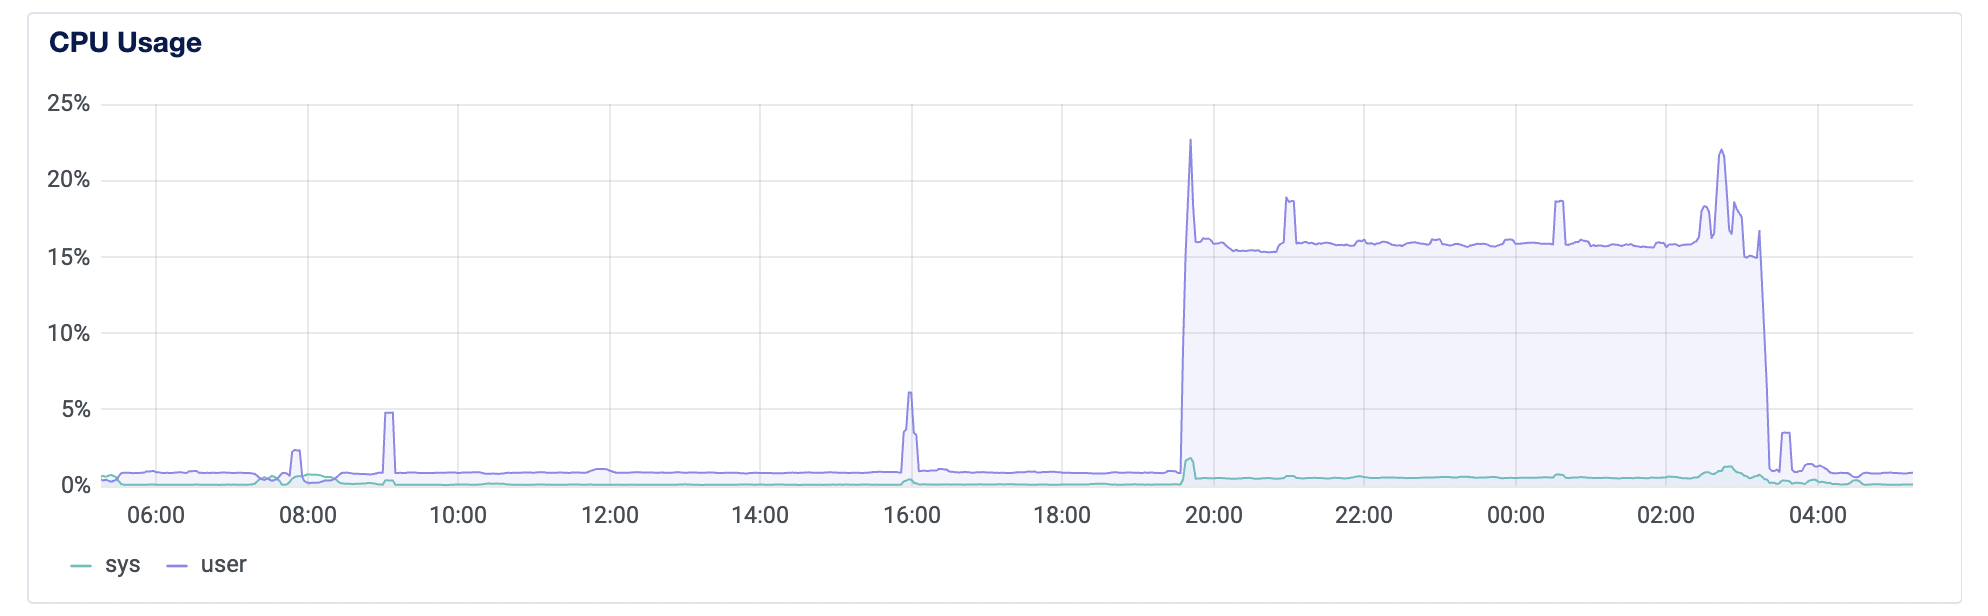
\includegraphics[width=\textwidth]{imagenes/implementacion/carga_cpu_docker_health_check.png}
\caption{Gráfico de carga de la CPU}
\label{fig:usoCPUProd}
\end{figure}

\section{Obras}
% https://github.com/daniharo/mordente/commit/da63c3b0

La última \textbf{épica} de historias de usuario que nos queda por comenzar a implementar es la relacionada con las \textbf{obras}: creación, visualización y eliminación. Sin embargo, hay una historia de usuario especial: se requiere gestionar archivos \texttt{PDF} de los usuarios, las partituras.


\subsection{Almacenando partituras: creación del \textit{bucket S3}}\label{subsection:crearBucket}

Con respecto al almacenamiento de las partituras, vamos a usar una solución estándar en la industria como son los \textit{buckets S3}. Un servicio de este tipo nos permite almacenar gran cantidad de ficheros de forma simple y referenciados por una clave: esto se conoce como \textbf{almacenamiento de objetos}. 

Como estamos usando el proveedor \textbf{Digital Ocean} que nos proporciona crédito gratuito, crearemos el \textit{bucket} en su propio servicio de almacenamiento de objetos, llamado \textbf{Digital Ocean Spaces}. Este proveedor llama a los \textit{buckets} \textbf{espacios}, pero al ser totalmente equivalentes y compartir la misma API, en este trabajo los denonimaremos con el nombre estandarizado de \textbf{bucket}.

El proceso de creación del \textit{bucket} para este proveedor es muy sencillo:

\begin{enumerate}
    \item Accedemos al panel de administración de \textbf{Digital Ocean}.
    \item Hacemos clic en \textbf{Create} y en \textbf{Spaces}.
    \item Dejamos la configuración por defecto ya que es adecuada a nuestro proyecto.
    \item Recibimos la confirmación de que el \textit{bucket} ya ha sido creado.
\end{enumerate}

\subsection{Intermediando entre el chat y Digital Ocean Spaces}
% https://github.com/daniharo/mordente/compare/1f448ef1...782e57b7
% https://github.com/daniharo/mordente/commit/da63c3b0fc8ca39ebd327965d9037ec885d4cd72

Una vez que tenemos el \textit{bucket} creado, solo necesitamos implementar la intermediación entre los usuarios y el \textit{bucket} para que puedan recibir y enviar las partituras dentro del mismo chat. Para ello, añadimos los paquetes \path{@aws-sdk/client-s3} y \path{@aws-sdk/s3-request-presigner} como dependencia, creados por \textbf{Amazon Web Services} y totalmente compatibles con cualquier servicio de almacenamiento de objetos S3 como el que usamos nosotros, \textbf{Digital Ocean Spaces}. También añadimos la dependencia \path{@grammyjs/files} que nos ayudará a manejar archivos que el bot envía o recibe.

\subsubsection{Pidiendo la partitura}

Para crear la obra en nuestra base de datos, implementamos la conversación \texttt{createSongConversation} que, tras preguntar por el nombre, pedirá al usuario que envíe el archivo de la partitura.

\subsubsection{Recibiendo partituras}

Cuando el bot recibe la partitura que ha enviado el usuario, la descarga en una ruta temporal\footnote{\url{https://grammy.dev/guide/files.html\#receiving-files}} y conecta con el \textit{bucket} para enviarle el archivo a la ruta \path{<id_agrupación>/<id_obra>/<nombre_archivo>.pdf} con la función \texttt{uploadFile}. Esta ruta nos permitirá asegurar que podemos mantener los nombres de los archivos sin que puedan colisionar entre sí.

\subsubsection{Enviando partituras}

Por defecto, todos los objetos que tenemos almacenados tienen acceso privado, es decir, solo el dueño del \textit{bucket} puede acceder a ellos. Por tanto, cuando un usuario pide una partitura, primero debemos generar una URL que está firmada por el dueño del \textit{bucket} y que permite el acceso durante un tiempo especificado a otros usuarios\footnote{\url{https://docs.aws.amazon.com/AmazonS3/latest/userguide/ShareObjectPreSignedURL.html}}. Esta URL temporal se enviará a la API de Telegram para enviar el archivo dentro del chat, mediante el método \texttt{replyWithDocument}\footnote{\url{https://grammy.dev/guide/files.html\#sending-files}}.

Los cambios en el código que implementan la creación de partituras y la comunicación con el \textit{bucket} están disponibles en \textbf{GitHub}\footnote{\textit{Commit:} \url{https://github.com/daniharo/mordente/compare/1f448ef1...782e57b7}}.

\subsection{Lógica común con agrupaciones y eventos}

Ya se pueden crear obras, por lo que ahora necesitamos necesitamos implementar la plantillas necesarias para visualizar la lista de obras (\texttt{song-list.pug}), el menú de la lista de obras (\texttt{songListMenu}) y el menú para el detalle de una obra (\texttt{songMenu})\footnote{\textit{Commit:} \url{https://github.com/daniharo/mordente/commit/da63c3b0}}. No se ha implementado una plantilla para el detalle de una obra ya que solo vamos a utilizar su nombre, por lo que una cadena de texto como respuesta es suficiente.

La implementación de estas funcionalidades se ha realizado siguiendo los pasos que se dieron tanto con las agrupaciones como con los eventos.

\subsection{Parametrizando los valores del \textit{bucket}}

% https://github.com/daniharo/mordente/commit/a5532a0454920ef41dd7f4c2bb87c6de1f88bd41

Para que el código se pueda usar con cualquier proveedor de servicios de almacenamiento de objetos, es necesario hacer que los datos de conexión al proveedor sean variables fáciles de cambiar.

Por ello vamos a añadir estos datos de conexión a las variables de entorno. En concreto, los datos que se necesita obtener del proveedor están explicados en la tabla \ref{tab:envS3}.

Si en el futuro se optara por otro proveedor, simplemente tendríamos que cambiar estas variables de entorno.

\begin{table}[]
    \centering
    \begin{tabular}{|l|c|}
        \hline
        \textbf{Variable de entorno} & \textbf{Significado} \\
        \hline
        \texttt{S3\_ENDPOINT} & Dominio en el que se encuentra el \textit{bucket} \\
        \hline
        \texttt{S3\_REGION} & Región en la que se aloja el \textit{bucket} \\
        \hline
        \texttt{S3\_BUCKET} & Nombre del \textit{bucket} que hemos creado \\
        \hline
        \texttt{S3\_KEY} & Clave de acceso al \textit{bucket} \\
        \hline
        \texttt{S3\_SECRET} & Clave secreta de acceso al \textit{bucket} \\
        \hline
    \end{tabular}
    \caption{Variables de entorno necesarias para configurar el \textit{bucket S3}.}
    \label{tab:envS3}
\end{table}


\section{Copias de seguridad de la base de datos}

% https://github.com/daniharo/mordente/compare/c4387aa8...2940907d

Todo sistema que pretenda ser \textbf{fiable} para los usuarios debe implementar un sistema de modo que si los datos se corrompen accidentalmente, la pérdida de datos esté controlada y no sea ilimitada: por ejemplo, que se pueda recuperar una versión anterior de una fecha concreta.

Esto lo podemos solucionar fácilmente añadiendo un nuevo servicio a la infraestructura montada en \texttt{docker compose}.

Haciendo una búsqueda, encontramos que la imagen de \texttt{docker} \path{eeshugerman/postgres-backup-s3} tiene lo que necesitamos: realiza una copia de seguridad en un \textit{bucket} de S3 (recordemos que hemos creado uno en la sección \ref{subsection:crearBucket}) con la configuración dada.

Las variables de configuración que le tenemos que proporcionar a este servicio son todas las relacionadas con el \textit{bucket S3}, explicadas en la tabla \ref{tab:envS3}, las relacionadas con el acceso a la base de datos, y las relativas a la copia de seguridad que se detallan en la tabla \ref{tab:envBackup}.

\begin{table}[]
    \centering
    \begin{tabular}{|l|c|}
        \hline
        \textbf{Variable de entorno} & \textbf{Significado} \\
        \hline
        \texttt{SCHEDULE} & Cada cuánto tiempo se realizará la copia \\
        \hline
        \texttt{BACKUP\_KEEP\_DAYS} & \makecell{Cuántos días queremos que se \\ mantengan las copias de seguridad} \\
        \hline
        \texttt{S3\_PREFIX} & Prefijo para guardar las copias en el \textit{bucket} \\
        \hline
    \end{tabular}
    \caption{Variables de entorno necesarias para configurar las copias de seguridad.}
    \label{tab:envBackup}
\end{table}

Tras añadirlo\footnote{\url{https://github.com/daniharo/mordente/compare/c4387aa8...2940907d}} comprobamos que siempre se mantienen 8 días de copias de seguridad, tal y como se puede comprobar en las figuras \ref{fig:backup1} y \ref{fig:backup2}. Es por esto que comprobamos que a la variable de entorno \texttt{BACKUP\_KEEP\_DAYS} realmente hay que sumarle 1 ya que especifica cuántas copias \textbf{anteriores} a la que se está creando en ese momento queremos mantener.

\begin{figure}[h]
\centering
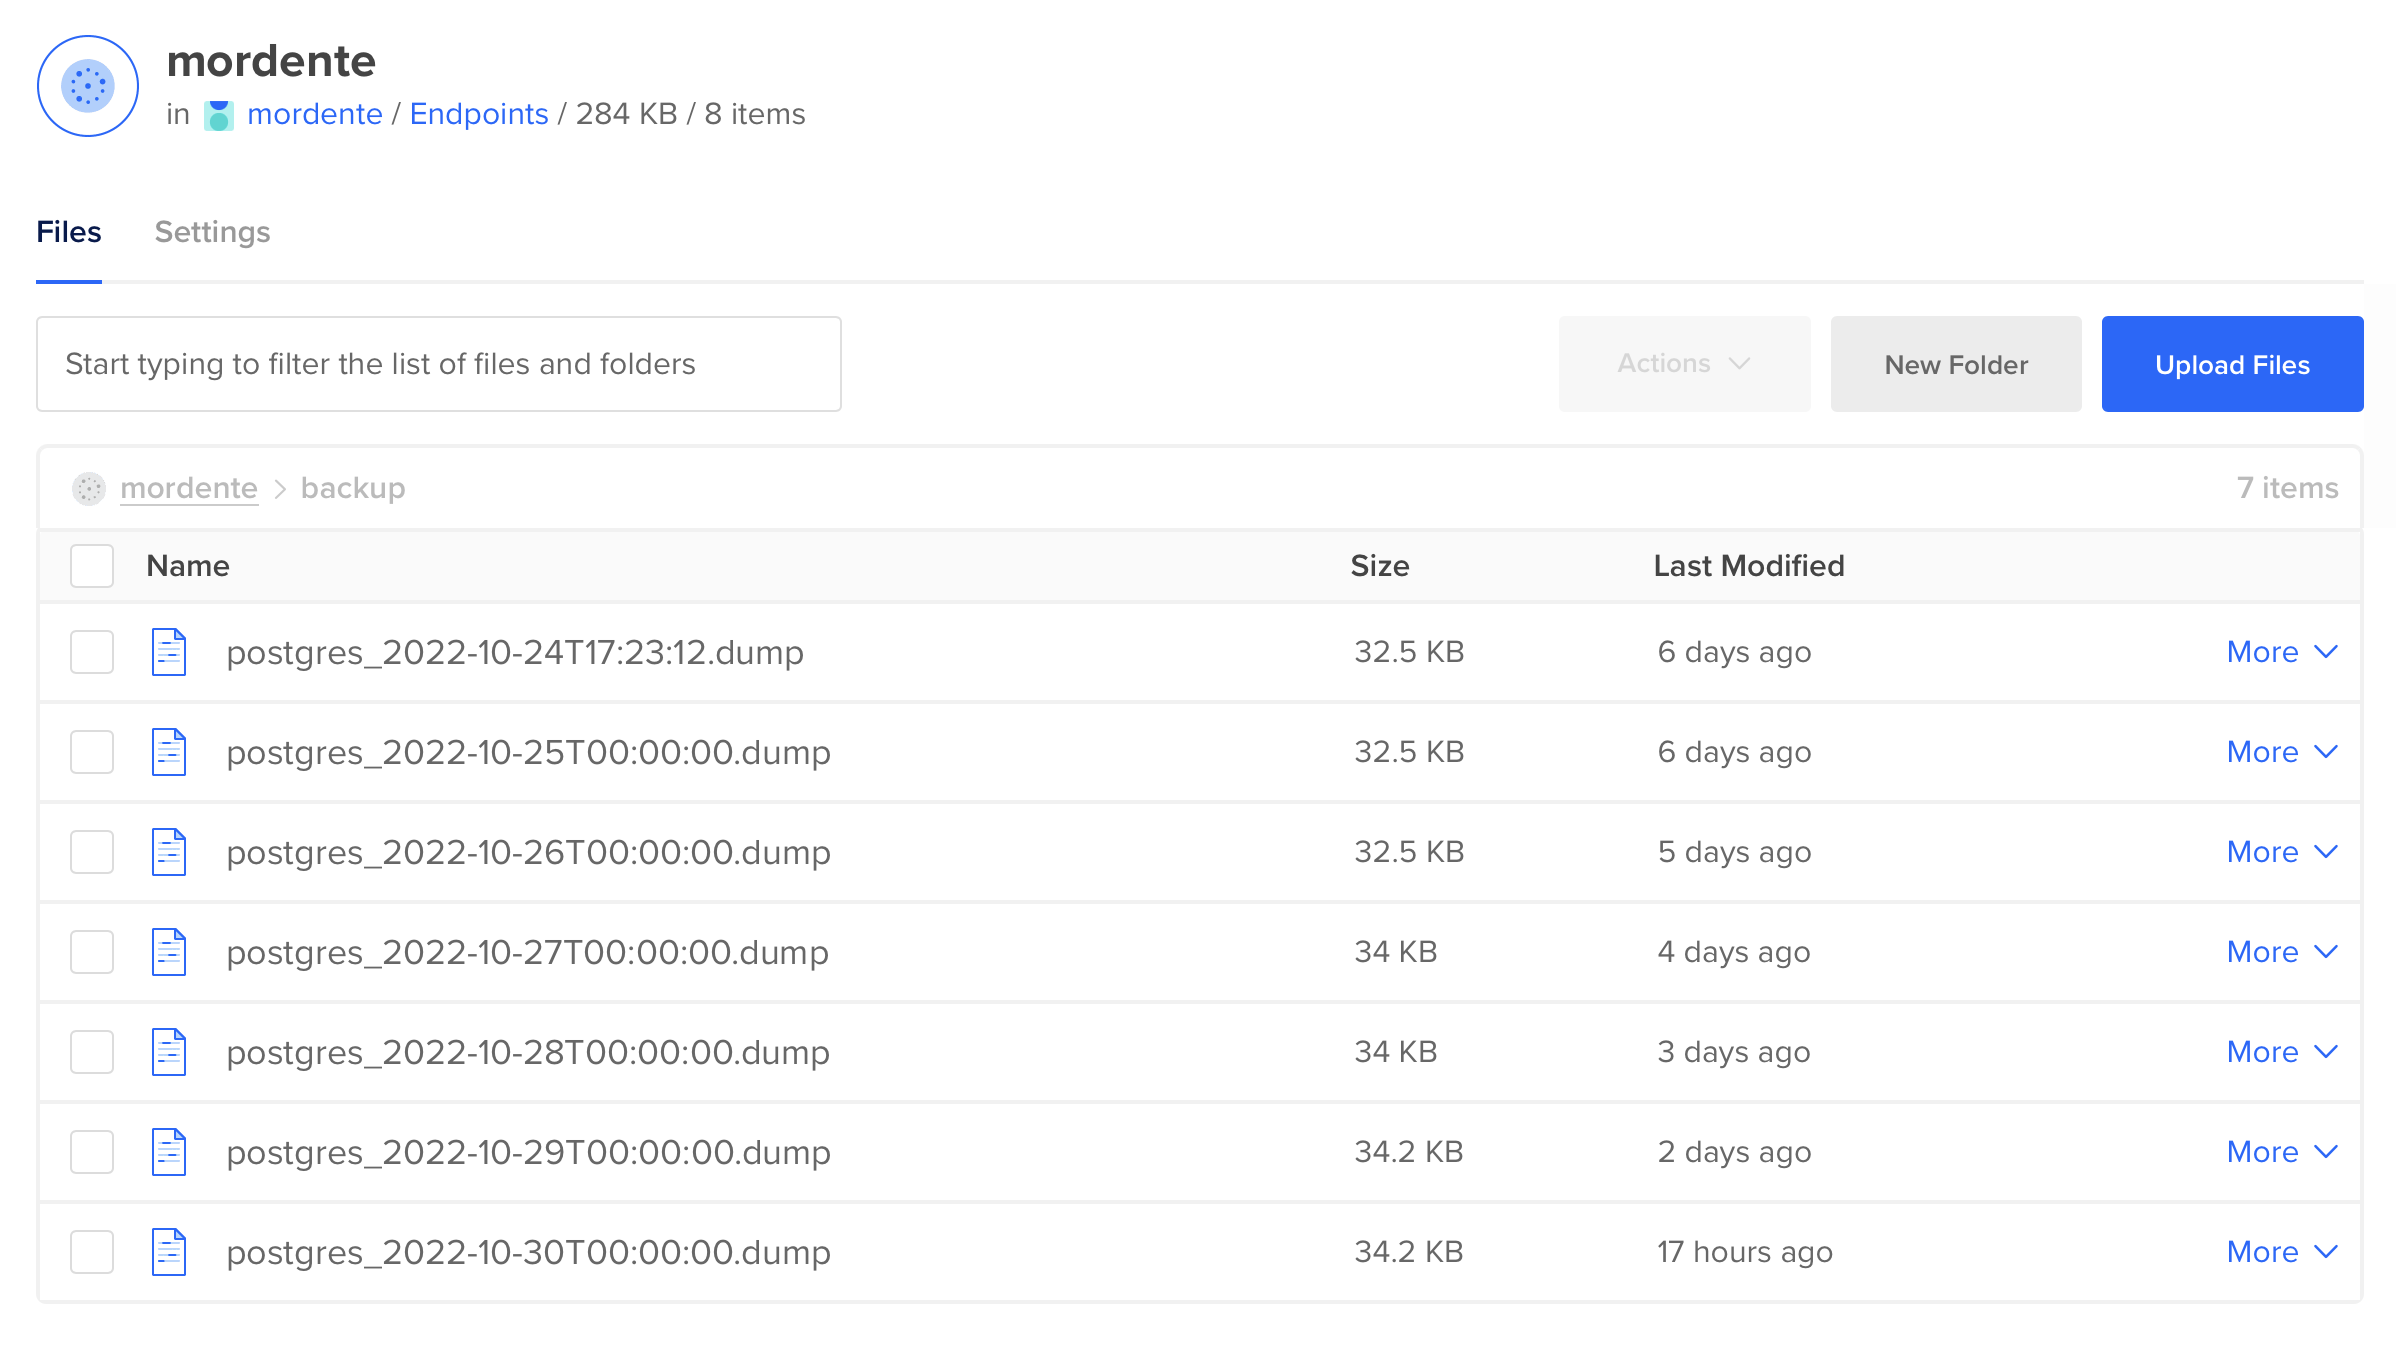
\includegraphics[width=0.75\textwidth]{imagenes/implementacion/backup_antes_de_borrado_automatico.png}
\caption{Archivos en el \textit{bucket S3} antes de superar el máximo de días configurado}
\label{fig:backup1}
\end{figure}

\begin{figure}[h]
\centering
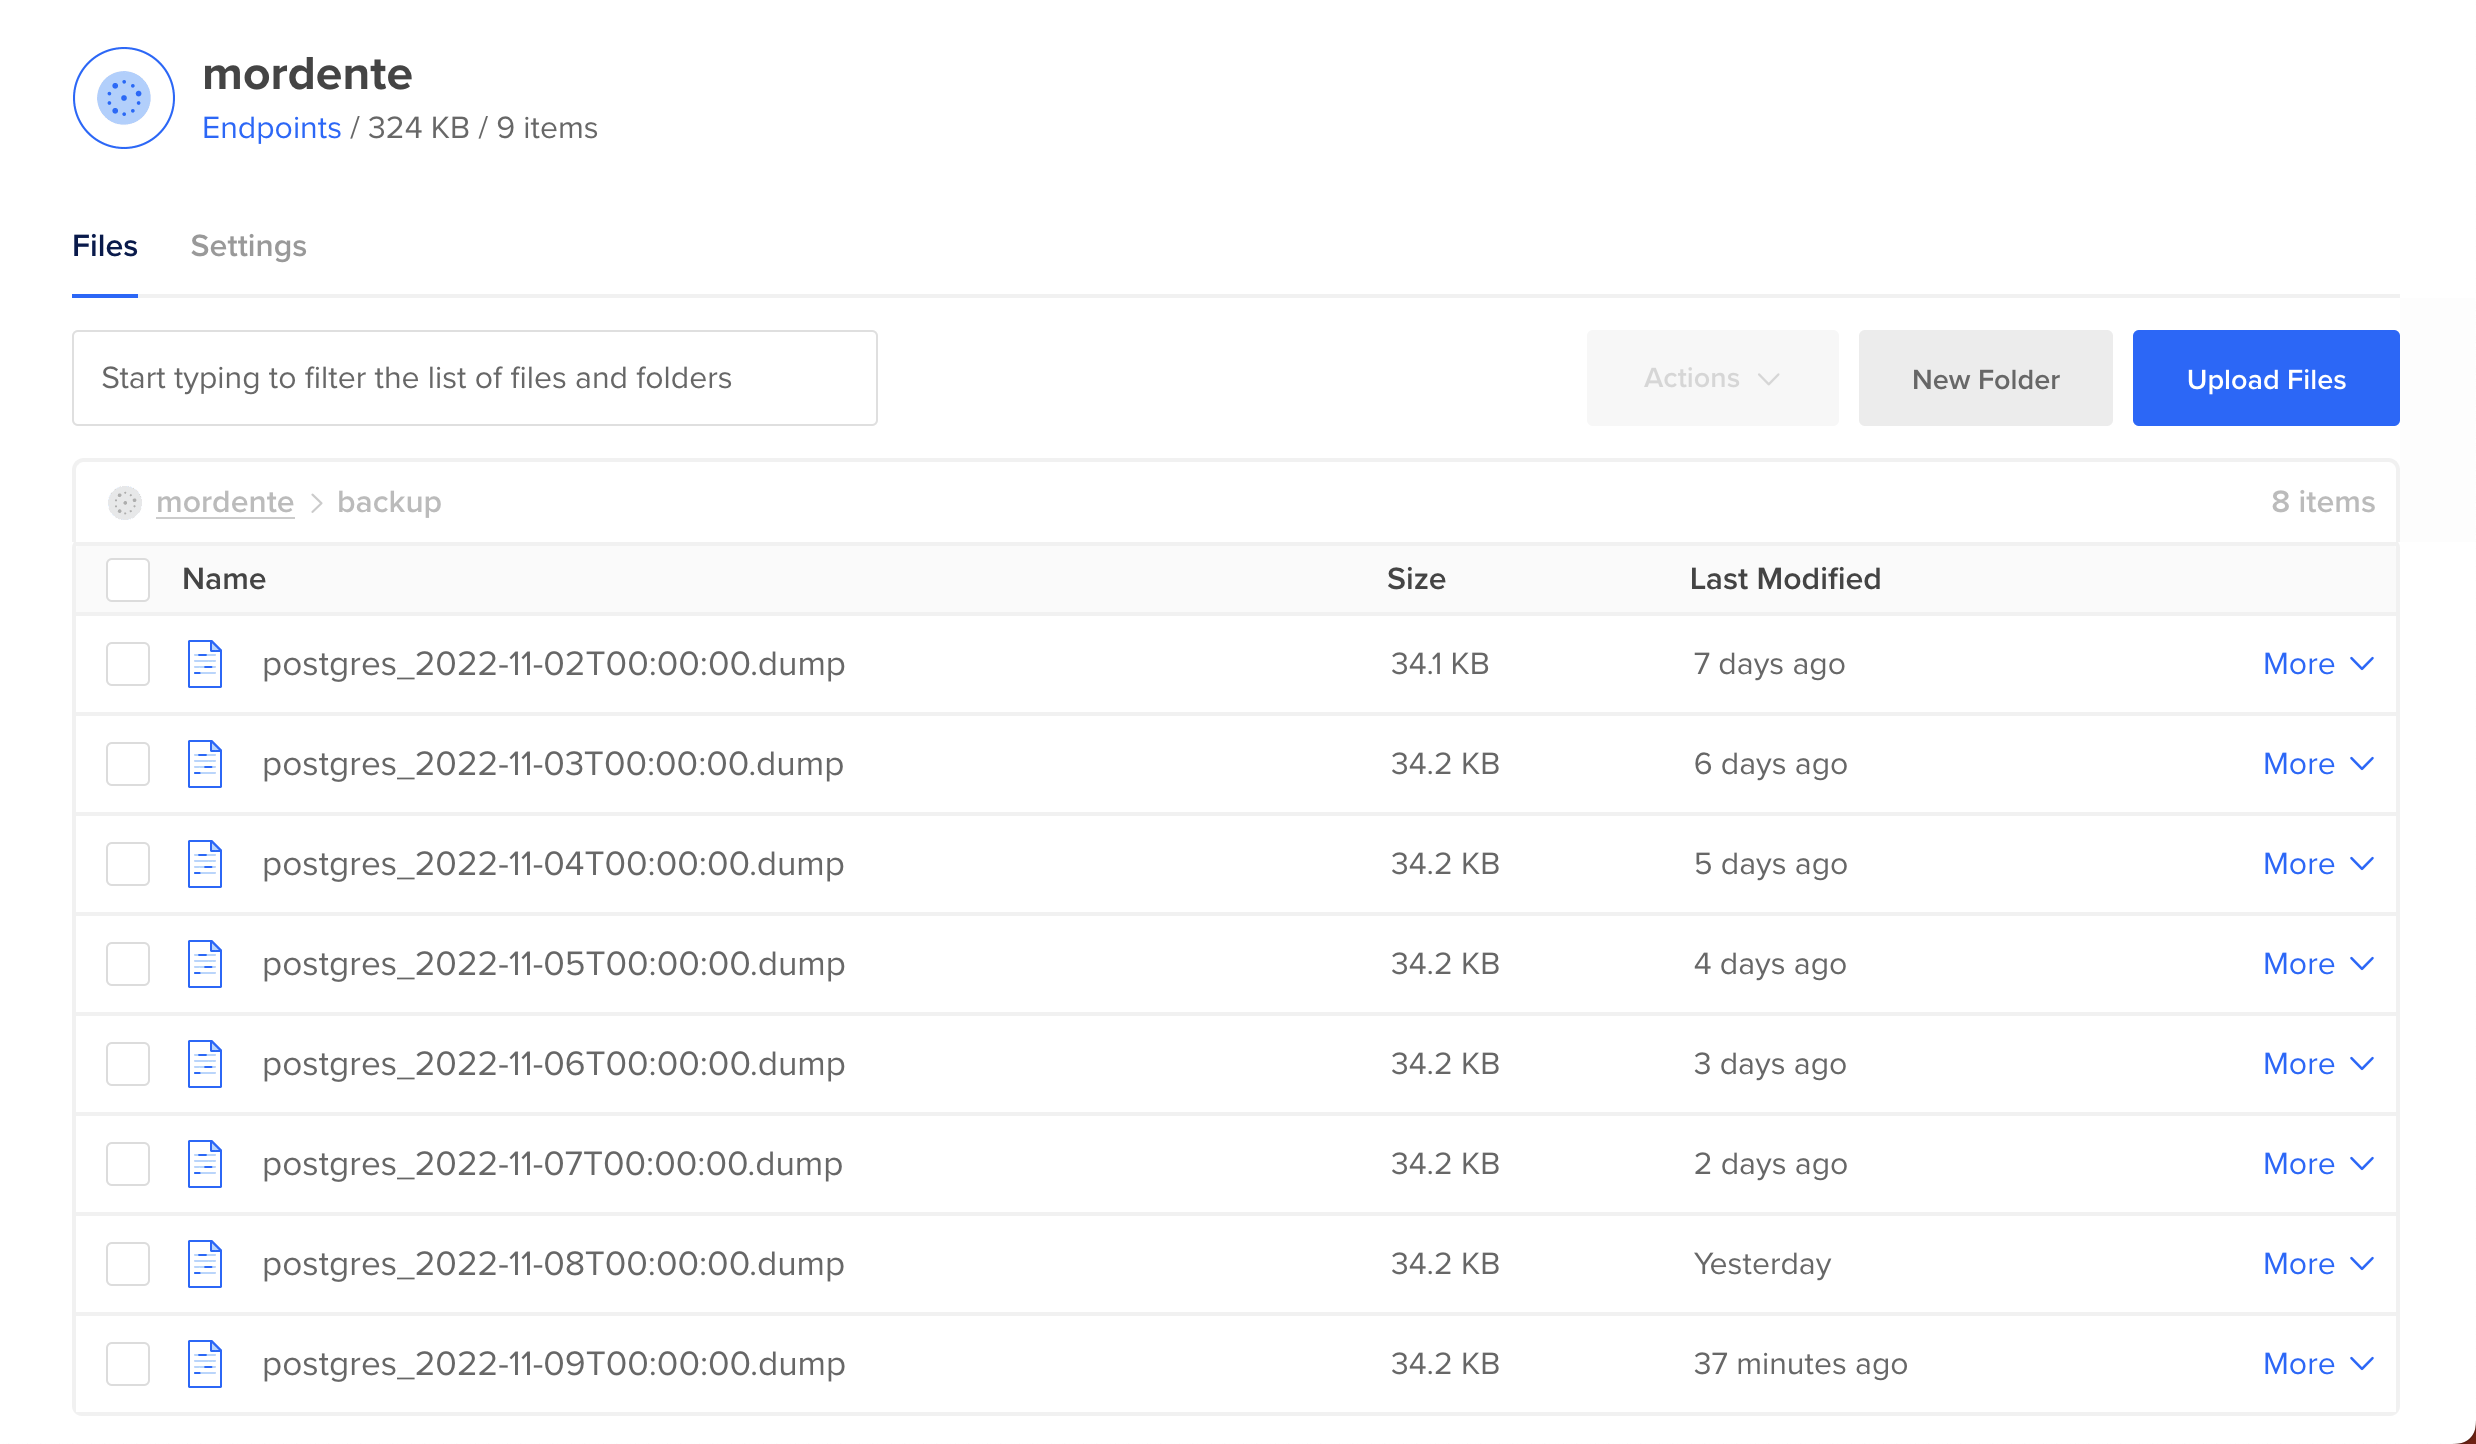
\includegraphics[width=0.75\textwidth]{imagenes/implementacion/backup_despues_borrado_automatico.png}
\caption{Archivos en el \textit{bucket S3} tras superar el máximo de días configurado}
\label{fig:backup2}
\end{figure}




\section{Despliegue Continuo (CD): Automatizando el despliegue del bot a producción}

% https://github.com/daniharo/mordente/commit/8965e0e893ea7ccf87da4947a8ba1ebf462d0c43

% https://github.com/daniharo/mordente/commit/6ade5d3554df9d49b8ece3adc08c54875c597397

Cuando cambiamos el código del proyecto, para actualizar el código que tenemos subido en el servidor de producción tenemos que seguir los siguientes pasos:

\begin{enumerate}
    \item Acceder mediante \texttt{ssh} al servidor.
    \item Actualizar el código con \texttt{git pull}.
    \item Reconstruir la imagen de \texttt{docker} usando el comando \texttt{docker compose up --build}.
\end{enumerate}

Dado que estos pasos se van a seguir de formar repetitiva cada vez que 

Es aquí cuando entra en juego el \textbf{Despliegue Continuo (CD)}: es una técnica que consiste en desplegar automáticamente la aplicación a producción cuando se realizan cambios (\textit{commits}) en el código\cite{Shahin_2017}. 
% https://arxiv.org/pdf/1703.07019.pdf

\textbf{GitHub} permite emplear esta técnica fácilmente mediante el uso de las llamadas \textbf{Github Actions}\footnote{\url{https://github.com/features/actions}}: mediante el añadido de ciertos archivos especiales al repositorio, \textbf{GitHub} ejecuta las acciones especificadas en los supuestos que configuremos.

En nuestro caso, queremos que cuando haya nuevo código en \textit{GitHub} para la rama \texttt{main} se ejecuten automáticamente los pasos reseñados en el comienzo de esta sección. Para ello, añadimos un archivo en la ruta \path{.github/workflows/deploy.yml}, en el cual especificamos cuándo queremos que se ejecute (en los \texttt{git push} a \texttt{main}), qué pasos hay que seguir, además de otras configuraciones que se pueden ver en el \textit{commit} correspondiente\footnote{\url{https://github.com/daniharo/mordente/commit/8965e0e8}}.

A partir de este momento, tal y como se puede ver en la figura \ref{fig:marcaDeploy}, a la derecha de cada \textit{commit} en \textbf{GitHub} aparece un símbolo a modo de marca de verificación en color verde, indicando que el despliegue se ha completado sin problemas. Al hacer clic aparece un botón de \textbf{Detalles} que nos permite consultar cómo se ha llevado a cabo el despliegue\footnote{Ejemplo: \url{https://github.com/daniharo/mordente/actions/runs/3416143998/jobs/5685987409}}.

Los datos para el acceso mediante \texttt{ssh} al servidor se almacenan cifrados como \texttt{Environment secrets}\footnote{\url{https://docs.github.com/en/actions/security-guides/encrypted-secrets}}, de modo que en ningún momento nadie más que el creador del proyecto tiene acceso a ellos. Además, solo los usuarios con permisos de escritura en la rama \texttt{main} pueden disparar un nuevo despliegue.


\begin{figure}[h]
\centering
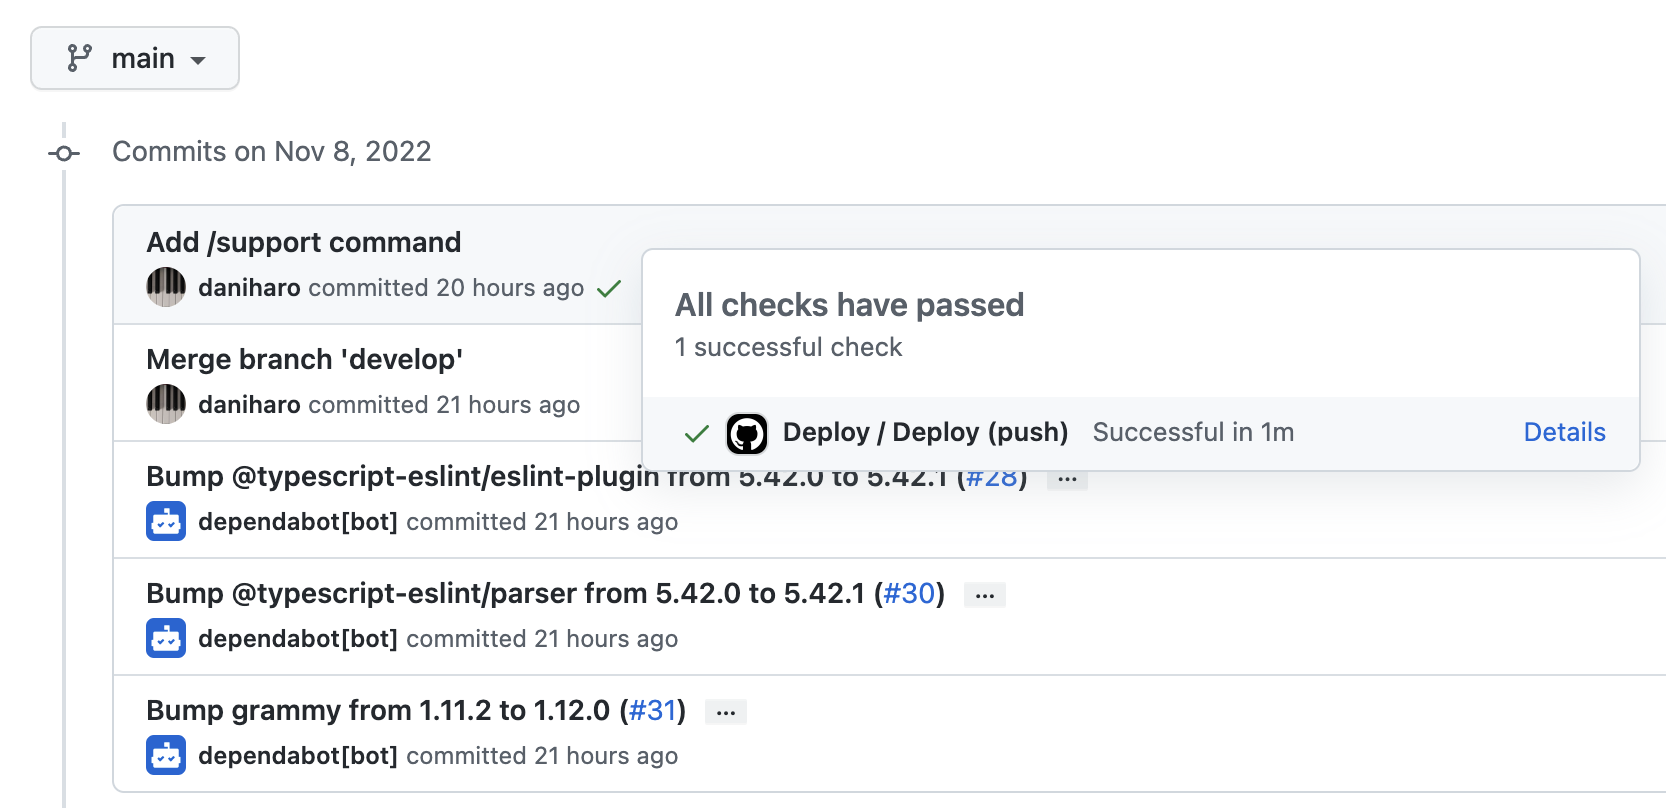
\includegraphics[width=0.75\textwidth]{imagenes/implementacion/marcaDeploy.png}
\caption{Marca de verificación del \textbf{Despliegue Continuo}}
\label{fig:marcaDeploy}
\end{figure}

Más tarde se ha implementado una configuración para que al modificar ciertos archivos como el \texttt{README.md} no se provoque un despliegue\footnote{\url{https://github.com/daniharo/mordente/commit/6ade5d35}}.


\section{Configurando la detección automática de vulnerabilidades}

% https://github.com/daniharo/mordente/commit/87541359abe2dc01ab819241ef8b595d729d21e7

Se ha detectado que una tarea frecuente durante el desarrollo de este proyecto ha sido revisar periódicamente de forma manual si alguna de las dependencias\footnote{Las dependencias del bot se especifican en el archivo \texttt{package.json}: \url{https://github.com/daniharo/mordente/blob/main/package.json}} usadas ha sido actualizada por haberse detectado alguna vulnerabilidad o por incorporar nuevas funcionalidades.

Es por ello que se ha configurado una herramienta automática que comprueba diariamente las dependencias y crea un \textit{Pull Request} para cada actualización. Esta herramienta la proporciona \textit{GitHub}, y su nombre es \textit{Dependabot}.

Para configurarla se ha añadido un archivo en la ruta \path{/.github/dependabot.yml}\footnote{\url{https://github.com/daniharo/mordente/commit/8754135}} especificando el intervalo entre detecciones (en nuestro caso cada día o \texttt{daily}), la ruta donde se encuentra el \texttt{package.json} con las dependencias y en qué rama queremos que se hagan los \textit{Pull Request} (\texttt{develop} ya que \textit{main} es la rama de producción).

Una vez configurado, comprobamos que cuando hay actualizaciones disponibles obtenemos las notificaciones correspondientes indicándolo\footnote{Ejemplo: \url{https://github.com/daniharo/mordente/pull/25}}.

\section{La función de editar}
% https://github.com/daniharo/mordente/commit/3e630b1fe45c479f836f21de003e7f6cc7f0bbee

La última funcionalidad que falta para que el bot sea usable es la de \textbf{editar} elementos, ya sean agrupaciones, eventos u obras. 

Dado que el tiempo restante para terminar el proyecto es limitado, se ha decidido implementar solo la edición de agrupaciones de forma que la edición de eventos y obras estaría preparada, solo pendiente de readaptar el código ya implementado.

El flujo del usuario será:
\begin{enumerate}
    \item Abrir el detalle de la agrupación.
    \item Pulsar el botón de ``Editar'' debajo del detalle, que solo aparecerá si es usuario administrador.
    \item Seleccionar en el menú qué atributo quiere editar.
    \item Responder al bot con el nuevo valor.
    \item Finalmente el usuario recibe una confirmación de que la agrupación ha sido modificada con éxito.
\end{enumerate}

\sloppy
Para ello, implementamos el menú para seleccionar qué atributo vamos a editar (\texttt{editEnsembleMenu}) y una nueva conversación para cada atributo que se puede editar: \texttt{editEnsembleNameConversation}, \texttt{editEnsembleDescriptionConversation}...

Los cambios en el código se pueden ver en el repositorio\footnote{\url{https://github.com/daniharo/mordente/commit/3e630b1}}.


\section{Página web: \href{https://mordente.es}{\texttt{mordente.es}}}

Una vez tenemos la aplicación funcionando y lista para poder hacer pruebas con usuarios, es conveniente desarrollar un sitio web donde explicar qué es Mordente, qué hace y cómo funciona. En esta sección se va a describir el proceso que se ha seguido para conseguirlo.

\subsection{Creación del proyecto}

Como venimos haciendo a lo largo del proyecto, hemos creado un repositorio público vacío en GitHub con el nombre de \texttt{mordente-docs}\footnote{\url{https://github.com/daniharo/mordente-docs}}. Seguidamente se ha clonado en el equipo de desarrollo usando el siguiente comando de \texttt{git}:

\begin{verbatim}
git clone git@github.com:daniharo/mordente-docs.git
\end{verbatim}

En la sección \ref{subsection:decisionDocumentacion} se ha decidido usar la herramienta \texttt{docusaurus} para desarrollar la página web, por lo tanto seguiremos sus instrucciones\footnote{\url{https://docusaurus.io/docs/installation}} para iniciar el desarrollo. Tras seguir las instrucciones, ya tenemos la estructura preparada para crear el contenido\footnote{\url{https://github.com/daniharo/mordente-docs/commit/1c25316}}.

\subsection{Creación de contenido}

La estructura de código que nos proporciona \texttt{docusaurus} nos permite configurar la estructura, apariencia y contenido de la página web partiendo de una plantilla \textit{responsive} (adaptada a todos los tamaños de pantalla) y accesible.

Aprovecharemos las posibilidades de configuración que nos ofrece \texttt{docusaurus} para cambiar los colores a nuestra paleta, añadir el logotipo y el contenido personalizado.

Algunas de las herramientas usadas durante este paso han sido:
\begin{itemize}
    \item \texttt{undraw}\footnote{\url{https://undraw.co/}}: es una extendsa biblioteca de ilustraciones SVG a las cuales se les puede personalizar fácilmente el color, y que representan distintas situaciones o ideas.
    \item \texttt{favicon-generator}\footnote{\url{https://www.favicon-generator.org/}}: el \texttt{favicon} es el icono que aparece a la izquierda del título de la página en el navegador. El archivo debe ubicarse en la raíz del directorio de la página y llamarse \texttt{favicon.ico}. Esta herramienta nos permite convertir cualquier imagen a un \texttt{favicon} con la medida adecuada.
    \item Se han usado algunos conocimientos previos de \texttt{react}\footnote{\url{https://reactjs.org/}}, ya que \texttt{docusaurus} está basado en esta biblioteca de interfaces de usuario.
\end{itemize}

En GitHub se pueden observar los cambios exactos realizados en el código para añadir el contenido de la página web\footnote{\url{https://github.com/daniharo/mordente-docs/compare/fd28973...e8980b0}}.



\subsection{Alojar en servidor}

Para que la página web esté accesible públicamente, es necesario alojarla en un servidor público. Existen múltiples plataformas que permiten alojar fácilmente contenido estático\footnote{Con \textit{contenido estático} nos referimos a archivos \texttt{HTML}, \texttt{CSS}, imágenes, etc. que se envían directamente al cliente sin necesidad de que haya una lógica en el servidor para calcularlos.} como el que genera \texttt{docusaurus}, pero las más interesantes permiten actualizar automáticamente el contenido del servidor cada vez que hay un \texttt{commit} en la rama principal del repositorio. Algunas de las más conocidas son:

\begin{itemize}
    \item \textbf{Vercel}\footnote{\url{https://vercel.com/}}: Es la empresa que desarrolla el \textit{framework} \texttt{Next.js}, una de las herramientas más usadas\footnote{\url{https://survey.stackoverflow.co/2022/\#most-popular-technologies-webframe}} por su flexibilidad para crear páginas web requieran de lógica en el servidor o no. Su servicio de alojamiento de páginas web destaca por su facilidad de uso, con una configuración automática e inmediata.
    \item \textbf{Netlify}\footnote{\url{https://www.netlify.com/}}: Principal competidor de Vercel, ofrece más posibilidades de configuración pero un peor rendimiento.
    \item \textbf{Github Pages}\footnote{\url{https://pages.github.com/}}: Es un servicio prestado por la forja de repositorios \textbf{GitHub}. Requiere de una configuración más compliacada para automatizar la compilación del código\footnote{\url{https://docusaurus.io/docs/deployment\#deploying-to-github-pages}}.
    \item \textbf{Cloudflare Pages}\footnote{\url{https://pages.cloudflare.com/}}: Nuevo servicio equivalente a Netlify o Vercel, con una configuración igual de sencilla. Es provisto por Cloudflare, una compañía especializada en prestar servicios de \textit{caché de contenido} y de seguridad.
\end{itemize}

Se optará por \textbf{Vercel} por la familiaridad del desarrollador de este proyecto con este proveedor por proyectos anteriores y por su facilidad de uso.

Para alojar nuestra página en \textbf{Vercel}, simplemente seguimos la documentación\footnote{\url{https://docusaurus.io/docs/deployment\#deploying-to-vercel}}, tarea que no nos lleva más de unos minutos. Una vez hemos terminado, tenemos la página web en una dirección asignada automáticamente: \url{https://mordente.vercel.app}.

\subsection{Redirecciones}

Para facilitar el acceso al contenido de este trabajo, se va a configurar el servidor de manera que al acceder a ciertas rutas se abra una determinada página de un dominio externo. Lo haremos siguiendo las instrucciones de Vercel para ello\footnote{\url{https://vercel.com/docs/project-configuration\#project-configuration/redirects}}. Las rutas que redireccionaremos están descritas en la tabla \ref{tab:redirecciones}.

\begin{table}[]
    \centering
    \begin{tabular}{|l|c|}
        \hline
        \textbf{Ruta origen} & \textbf{Redirige permanentemente a} \\
        \hline
        \href{https://mordente.es/repo}{\texttt{/repo}} & \multirow{2}{*}{Código del bot} \\ \cline{1-1}
        \href{https://mordente.es/source}{\texttt{/source}} & \\ \hline
        \href{https://mordente.es/source/docs}{\texttt{/source/docs}} & Código de la página web \\
        \hline
        \href{https://mordente.es/source/memoria}{\texttt{/source/memoria}} & Código \LaTeX{} de la memoria \\
        \hline
        \href{https://mordente.es/memoria}{\texttt{/memoria}} & Memoria en formato \texttt{PDF} \\
        \hline
        \href{https://mordente.es/try}{\texttt{/try}} & Bot en Telegram \\
        \hline
    \end{tabular}
    \caption{Redirecciones en \href{https://mordente.es}{\texttt{mordente.es}}}
    \label{tab:redirecciones}
\end{table}

\subsection{Asignación de dominio}\label{subsection:asignacionDominio}

Registrar un dominio personalizado nos permitirá acceder a la página con una dirección sencilla y fácil de recordar. 

Las empresas encargadas de registrar un dominio son llamadas \textbf{registradores de dominios}. Tras comparar precios entre diversos registradores para dominios \texttt{.es}, en nuestro caso se opta por \textbf{IONOS}\footnote{\url{https://www.ionos.es/dominios/}}, que ofrece el dominio \texttt{mordente.es} por 1,21\texteuro{} el primer año, la mejor oferta entre las encontradas.

Tras hacer el proceso de compra, seguimos las instrucciones\footnote{\url{https://vercel.com/docs/concepts/projects/domains/add-a-domain}} de \textbf{Vercel} para asignar el dominio al proyecto. Esperamos un tiempo aproximado de una hora mientras se propagan los nuevos registros DNS, tras el cual Vercel genera automáticamente el certificado TLS para nuestro dominio\footnote{\url{https://vercel.com/blog/automatic-ssl-with-vercel-lets-encrypt}} y podemos acceder sin problemas a \url{https://mordente.es}.

El último paso es modificar la configuración de \texttt{docusaurus} para ajustar correctamente el nuevo dominio principal\footnote{\url{https://github.com/daniharo/mordente-docs/commit/c2e2f8e}}.

\subsection{Probando otros proveedores}

Durante la realización de un proyecto personal paralelo\footnote{Aplicación usando ingeniería inversa para consultar en tiempo real los tiempos de paso del Metropolitano de Granada: \url{https://metrogranada.pages.dev}. Código en \url{https://github.com/daniharo/Metro-Granada-Webapp}.} se ha comprobado cómo \textbf{Cloudflare Pages}, siendo un proveedor muy parecido a \textbf{Vercel}, proporciona un menor tiempo de respuesta (aproximadamente la mitad) a la hora de alojar un servidor \texttt{Next.js}\footnote{\url{https://nextjs.org/}} que incluye \textit{Rutas API Edge}\footnote{\url{https://nextjs.org/docs/api-routes/edge-api-routes}}.


Es por esto que se ha querido comprobar si para sitios puramente estáticos como el que hemos creado en esta sección, \textbf{Cloudflare Pages} es capaz también de dar un mayor rendimiento.

Para ello, se han seguido las instrucciones correspondientes, primero para alojar el contenido \footnote{\url{https://developers.cloudflare.com/pages/framework-guides/deploy-a-docusaurus-site/}} y después para asignar el dominio que creamos en la sección \ref{subsection:asignacionDominio}\footnote{\url{https://developers.cloudflare.com/pages/platform/custom-domains/}}. Por último se han añadido las redirecciones en el formato requerido por Cloudflare\footnote{\url{https://developers.cloudflare.com/pages/platform/redirects/}} (y que coincide con \textbf{Netlify}\footnote{\url{https://docs.netlify.com/routing/redirects/}}).


\subsubsection{Conclusiones del cambio de proveedor}

Tras seguir las instrucciones, hemos podido comprobar que aunque por culpa de una configuración por defecto incorrecta\footnote{\url{https://stackoverflow.com/a/74341851/12210701}} parecía que habíamos empeorado el rendimiento, tras solucionar la configuración sí que se ha mejorado el tiempo de respuesta con respecto a Vercel, aunque en una proporción despreciable (unos 120ms en Cloudflare frente a 140ms en Vercel).

Sin embargo, estas mediciones se hicieron por la noche, mientras la mayoría mediciones hechas durante el día indican que \textbf{Cloudflare} necesita un mayor tiempo para entregar la web: unos 250ms, frente a 140ms en Vercel.

Se ha detectado que el motivo es que, para reducir la carga de algunos centros de datos, algunas peticiones a páginas que están en el plan gratuito se enrutan a centros de datos lejanos\footnote{\url{https://community.cloudflare.com/t/peering-why-dont-i-reach-the-closest-datacenter-to-me/76479}}. En nuestro caso, hemos visto peticiones dirigidas a centros de datos en India o Estados Unidos, mientras que \textbf{Vercel} enruta todas las peticiones a Frankfurt (Alemania).

Es por esto que se ha decidido revertir el cambio de proveedor.


\section{Creación de dirección de email}

El proveedor de DNS utilizado para \texttt{mordente.es} nos permite obtener una dirección de correo electrónico gratuita con 2GB de almacenamiento. Por tanto, se ha creado una dirección 
de soporte (\texttt{soporte@mordente.es}) para los usuarios que puedan tener alguna consulta.

\section{Registro remoto de errores}\label{subsection:sentry}

Por último, vamos a configurar el servicio \textbf{Sentry} para poder obtener en tiempo real registros de los errores que se estén produciendo en la aplicación.

Seguimos los siguientes pasos:

\begin{enumerate}
    \item Creamos una cuenta gratuita en \url{https://sentry.io/signup/}.
    \item Creamos un nuevo proyecto para la plataforma \texttt{Node.js} (figura \ref{fig:sentryCreandoProyecto}).
    \item Añadimos las dependencias \path{@sentry/node} y \path{@sentry/tracing} a nuestro proyecto con \texttt{yarn add}.
    \item Copiamos el código generado en la página web (figura \ref{fig:sentryCodigoGenerado}) a nuestro código en el archivo \path{src/Sentry.ts}.
    \item Configuramos \textbf{Sentry} para que en los registros aparezca información de qué usuario ha manifestado el error y qué mensaje estábamos manejando. Crearemos un nuevo \texttt{middleware} llamado \texttt{useSentry} para ello.
\end{enumerate}

Tras la configuación\footnote{\textit{Commit:} \url{https://github.com/daniharo/mordente/commit/1753061f}}, la página de \textbf{Sentry} nos indica que está esperando al primer error, como se puede ver en la figura \ref{fig:sentryEsperandoLog}. Introducimos una llamada a una función que no existe, \texttt{foo()}, para comprobar que el error se registra correctamente.

En la página del proyecto en \textbf{Sentry} podemos observar que los registros se guardan y podemos ver la información correspondiente, como se muestra en la figura \ref{fig:sentryLog}.

\begin{figure}[h]
\centering
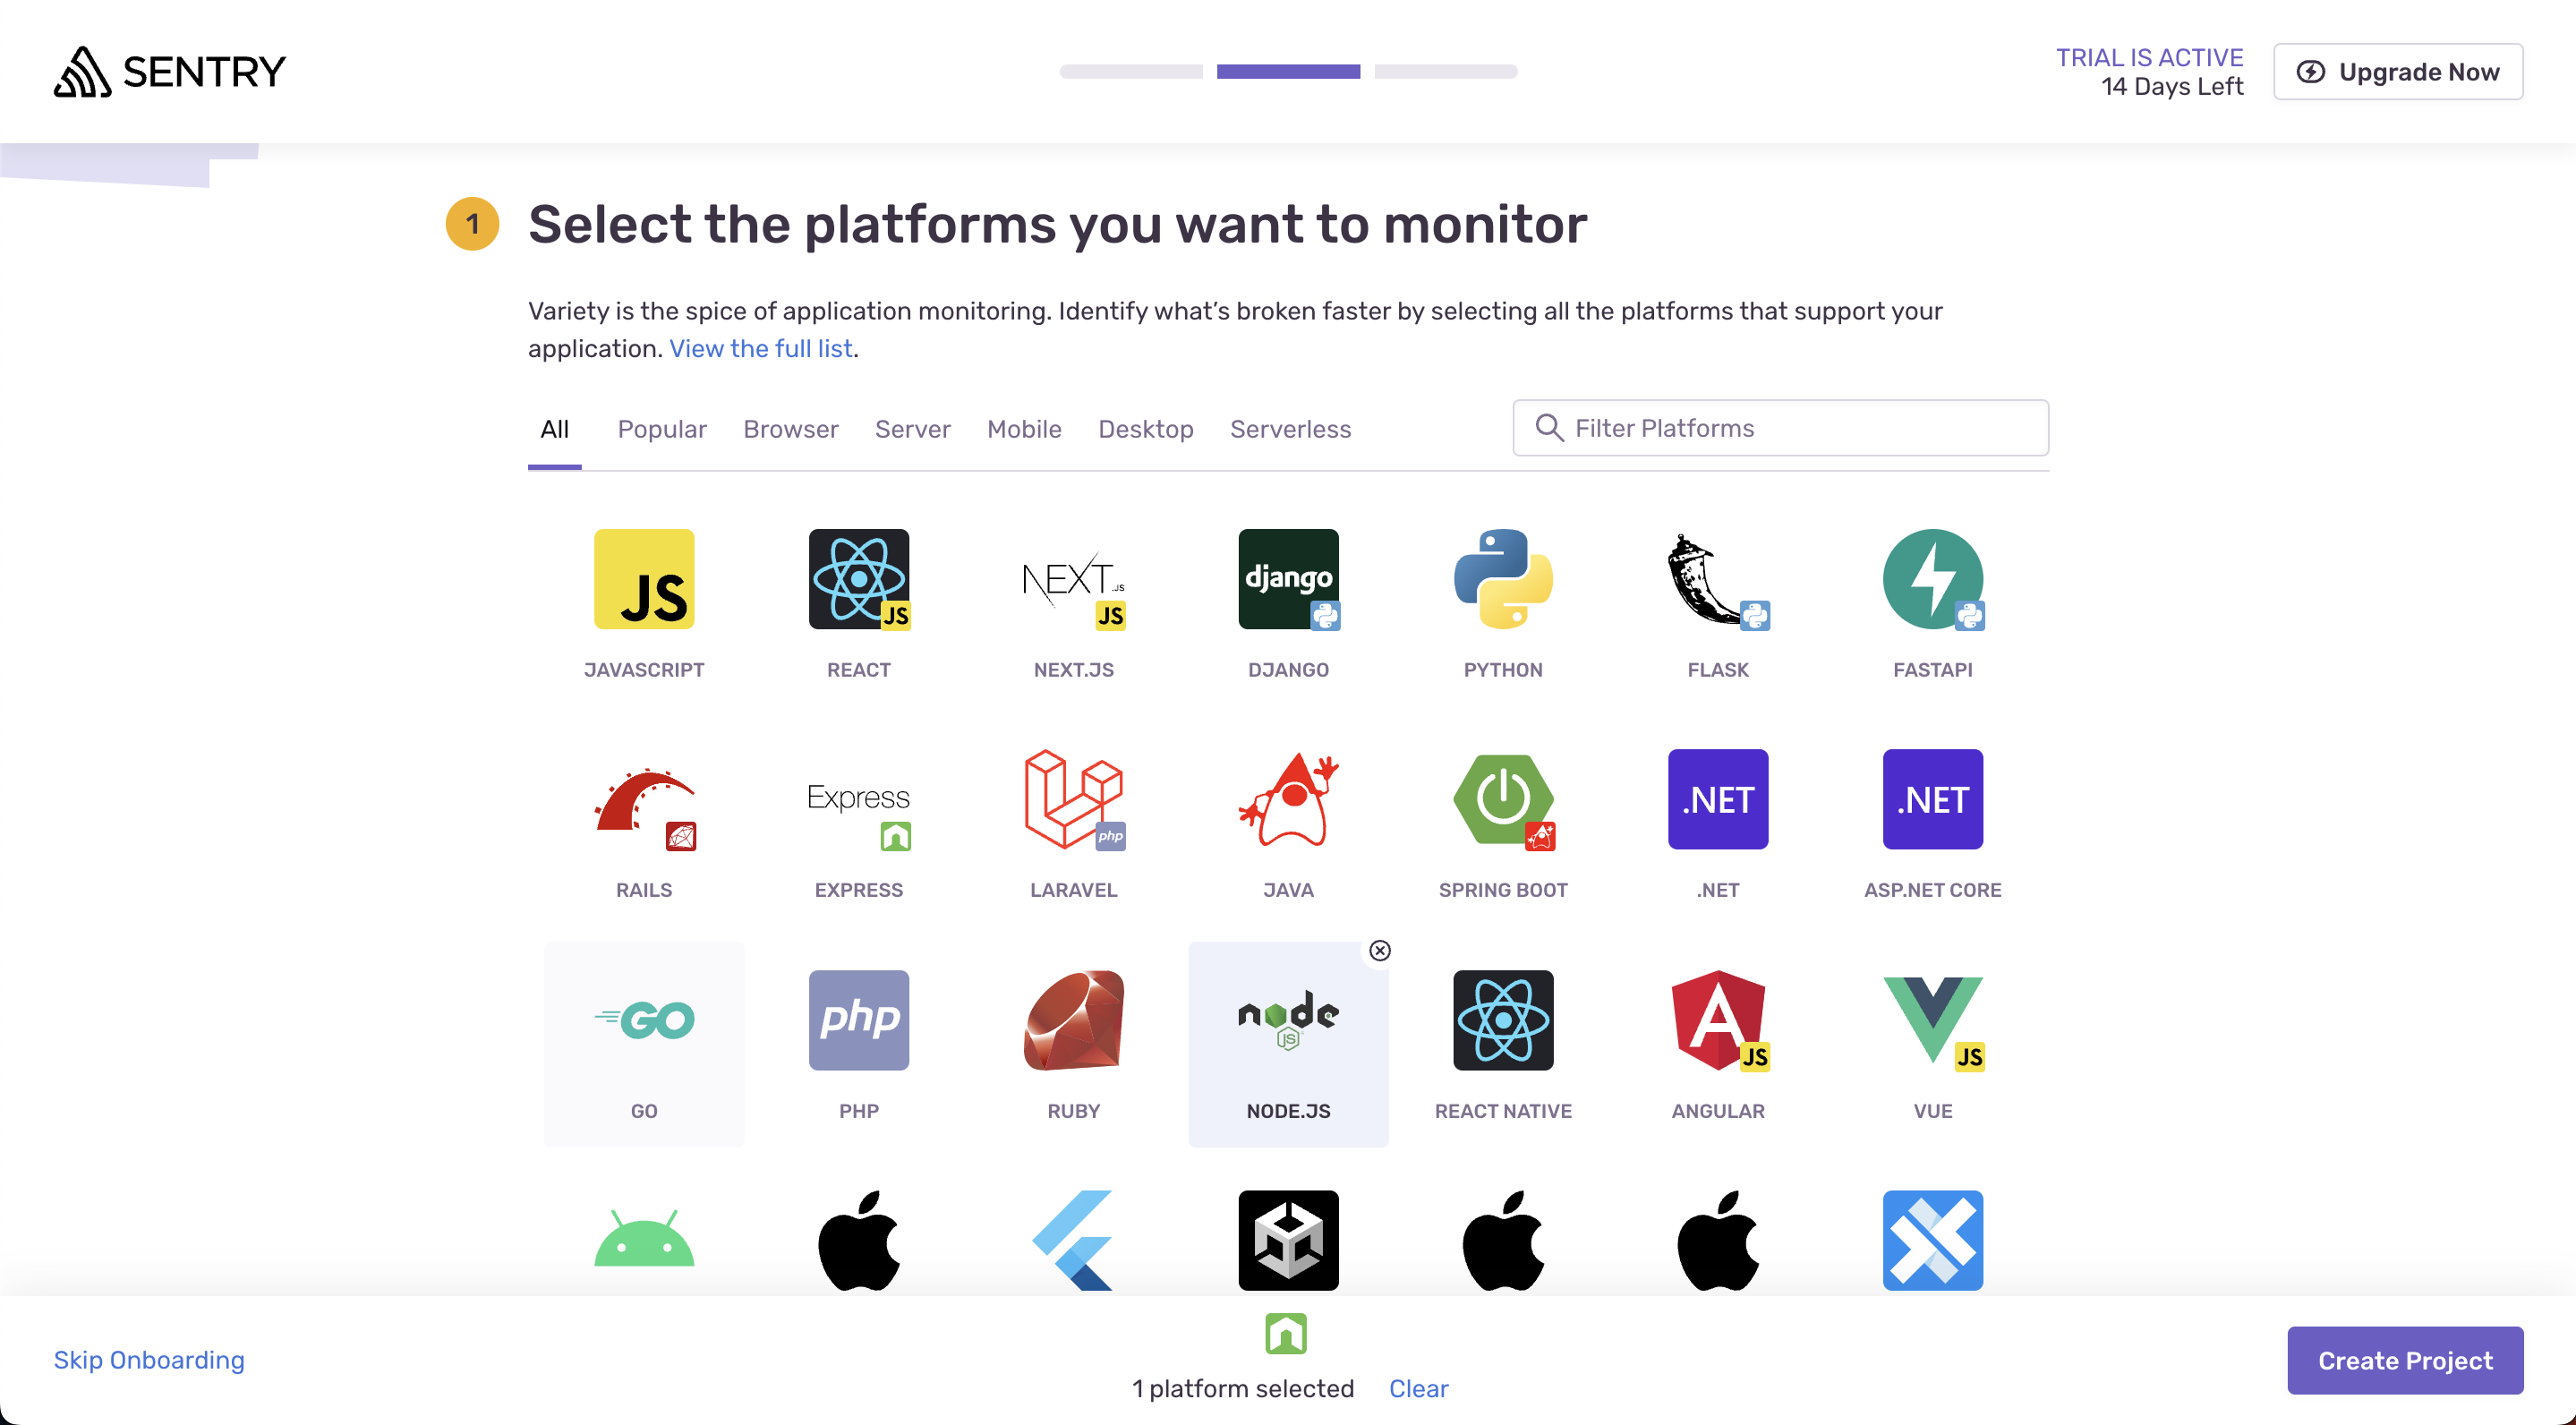
\includegraphics[width=0.75\textwidth]{imagenes/implementacion/sentry_creando_proyecto.png}
\caption{Creando el proyecto de \textbf{Sentry}}
\label{fig:sentryCreandoProyecto}
\end{figure}

\begin{figure}[h]
\centering
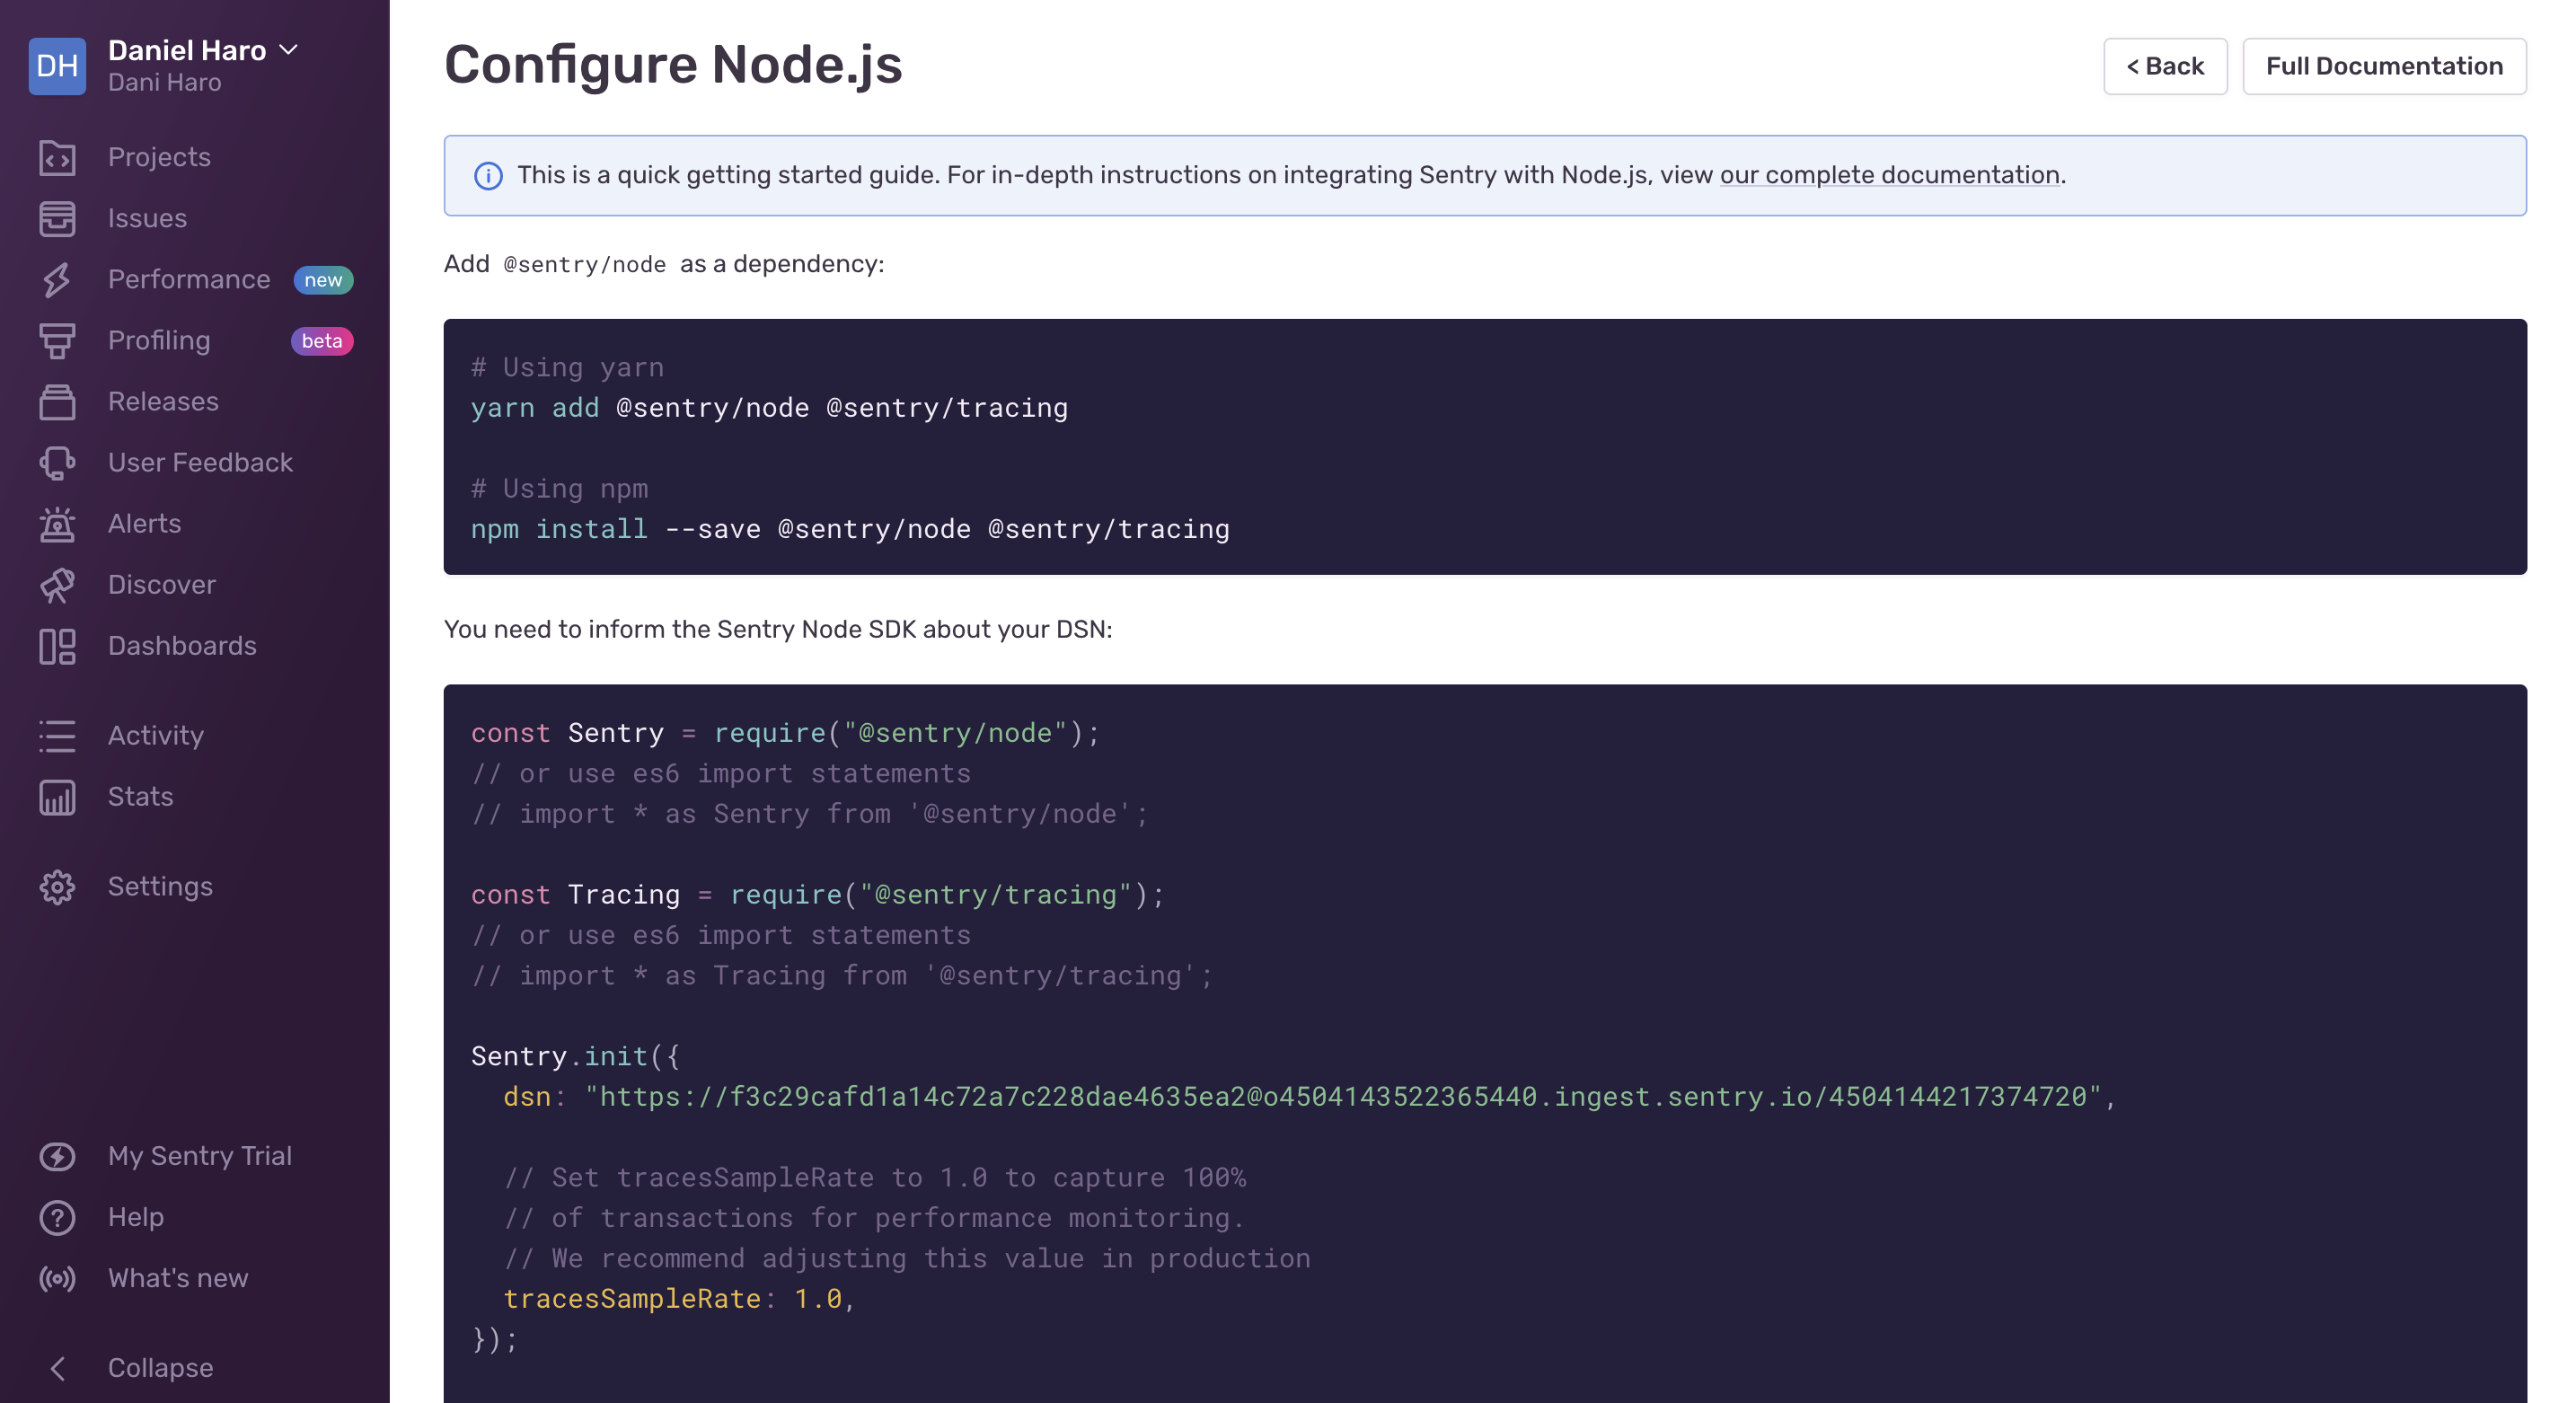
\includegraphics[width=0.75\textwidth]{imagenes/implementacion/sentry_codigo_generado.png}
\caption{Código generado por \textbf{Sentry} para incluir en un proyecto}
\label{fig:sentryCodigoGenerado}
\end{figure}

\begin{figure}[h]
\centering
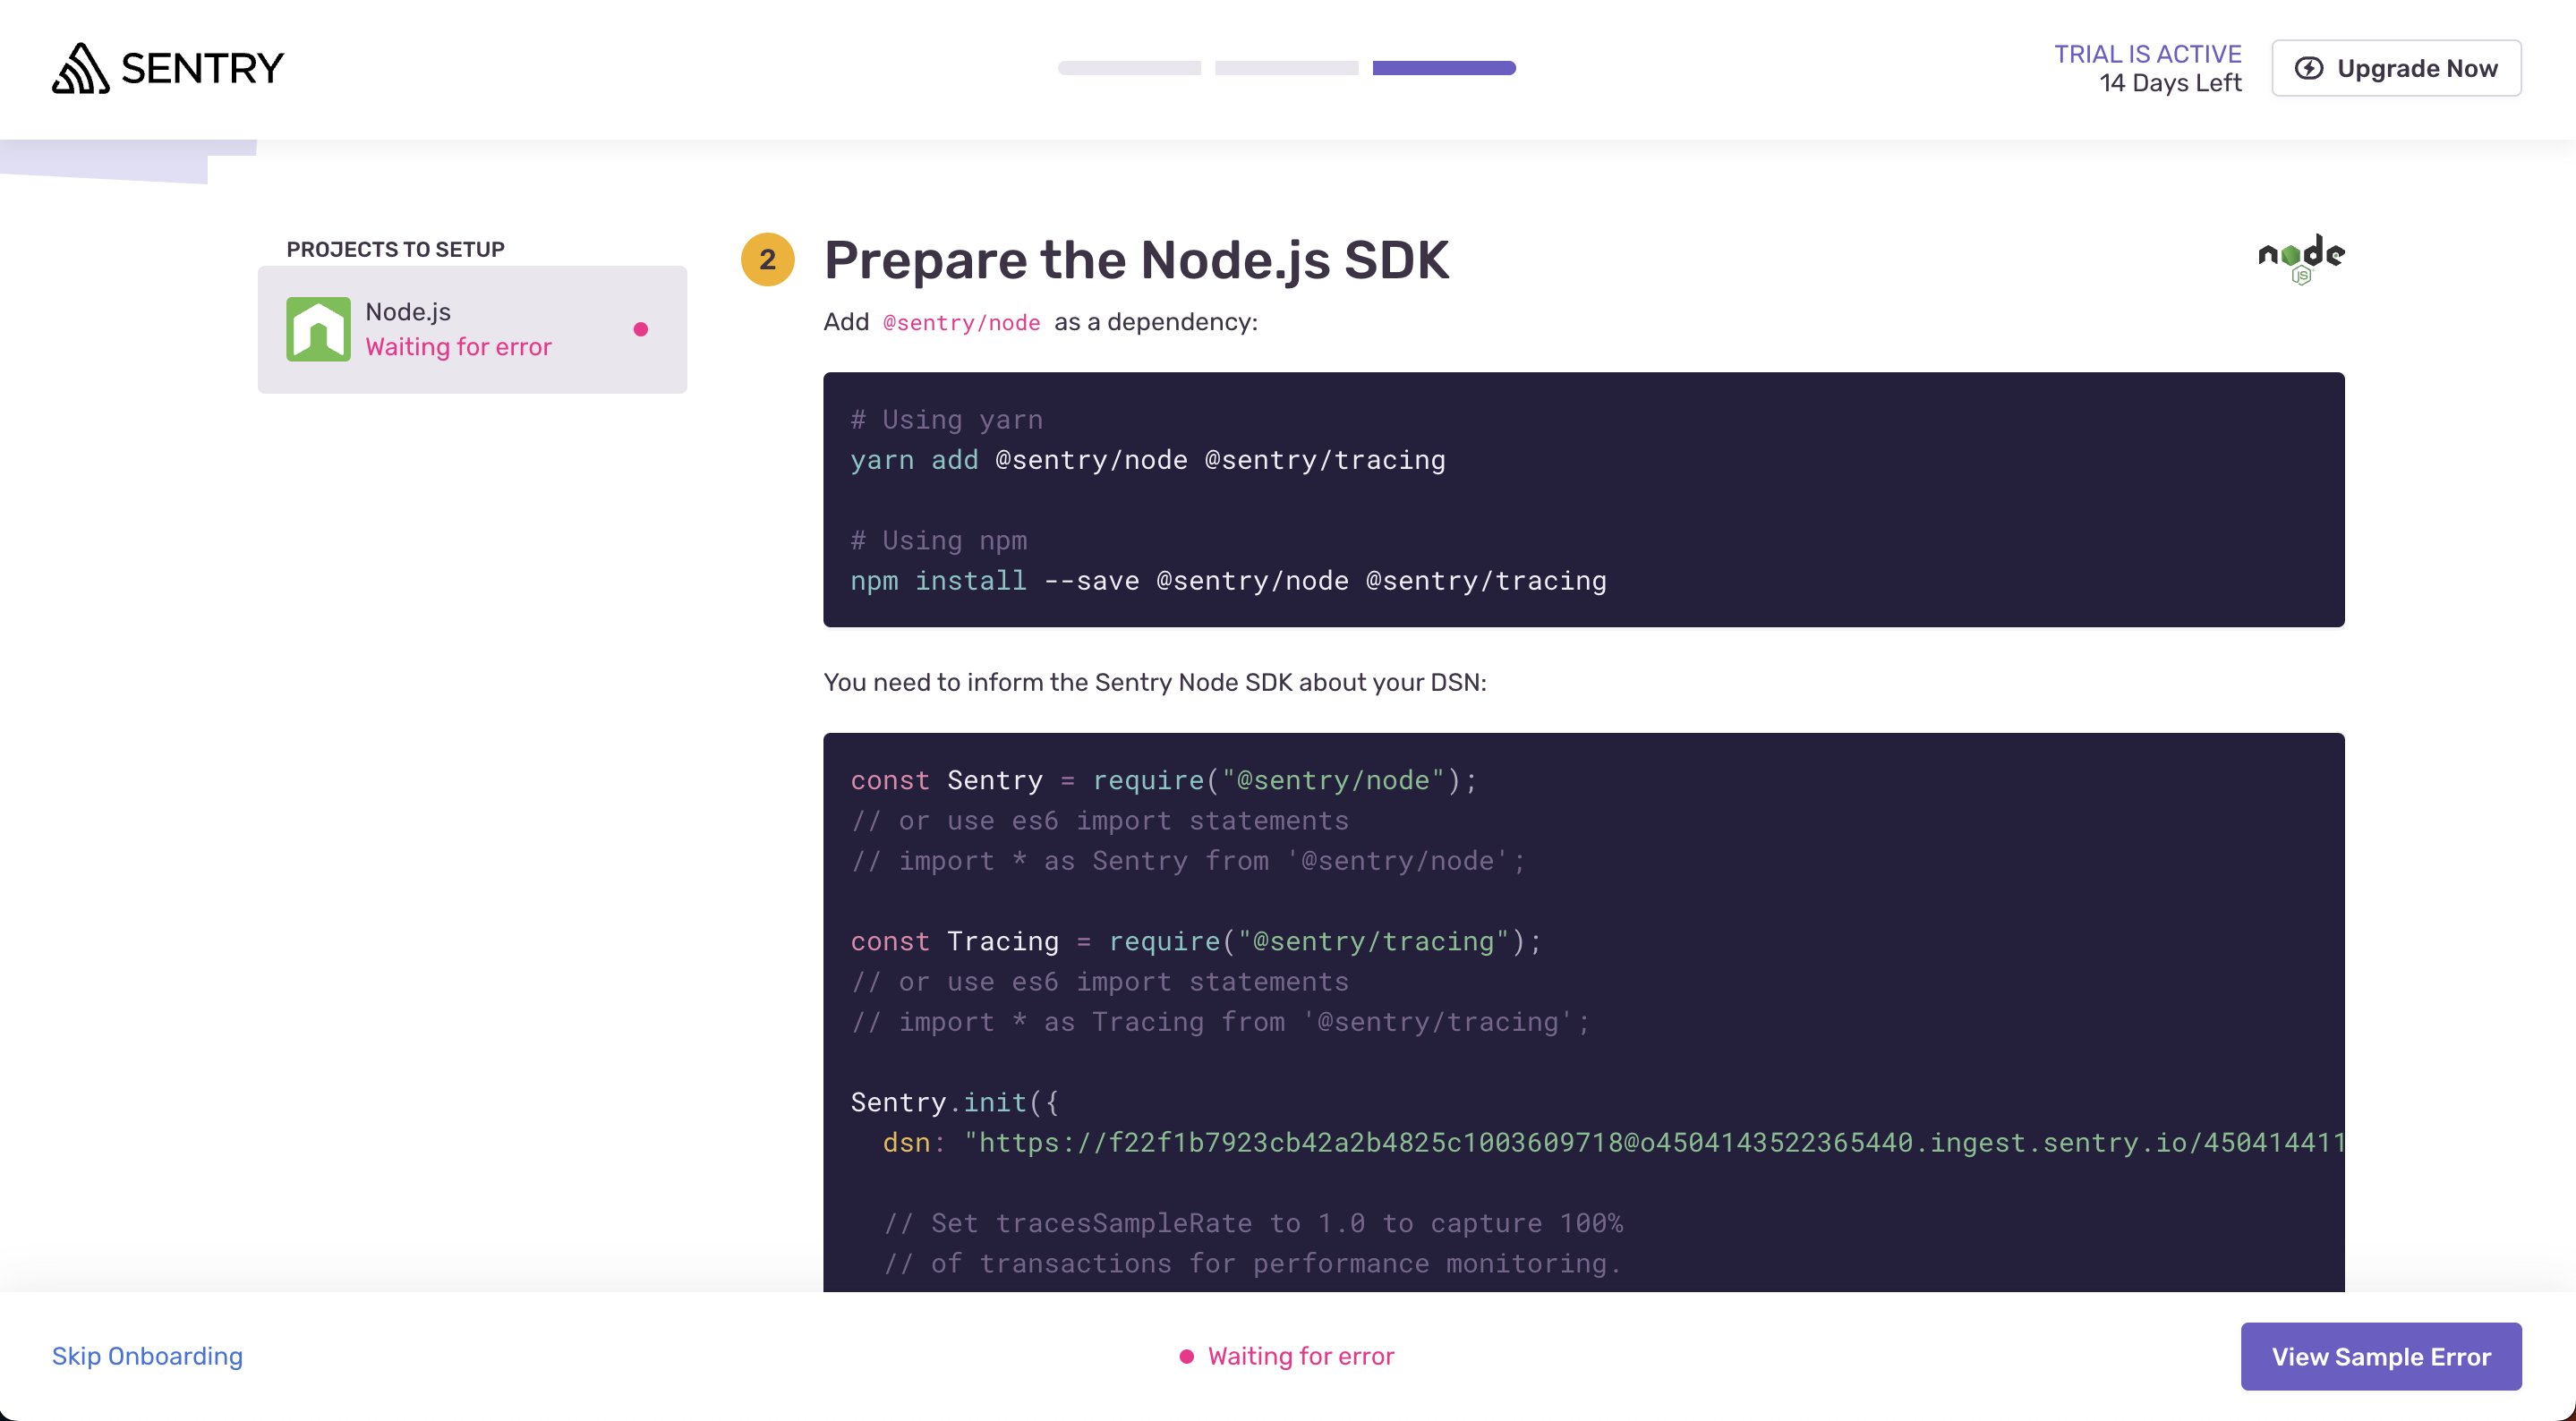
\includegraphics[width=0.75\textwidth]{imagenes/implementacion/sentry_esperando_log.png}
\caption{Esperando al primer log de \textbf{Sentry}}
\label{fig:sentryEsperandoLog}
\end{figure}

\begin{figure}[h]
\centering
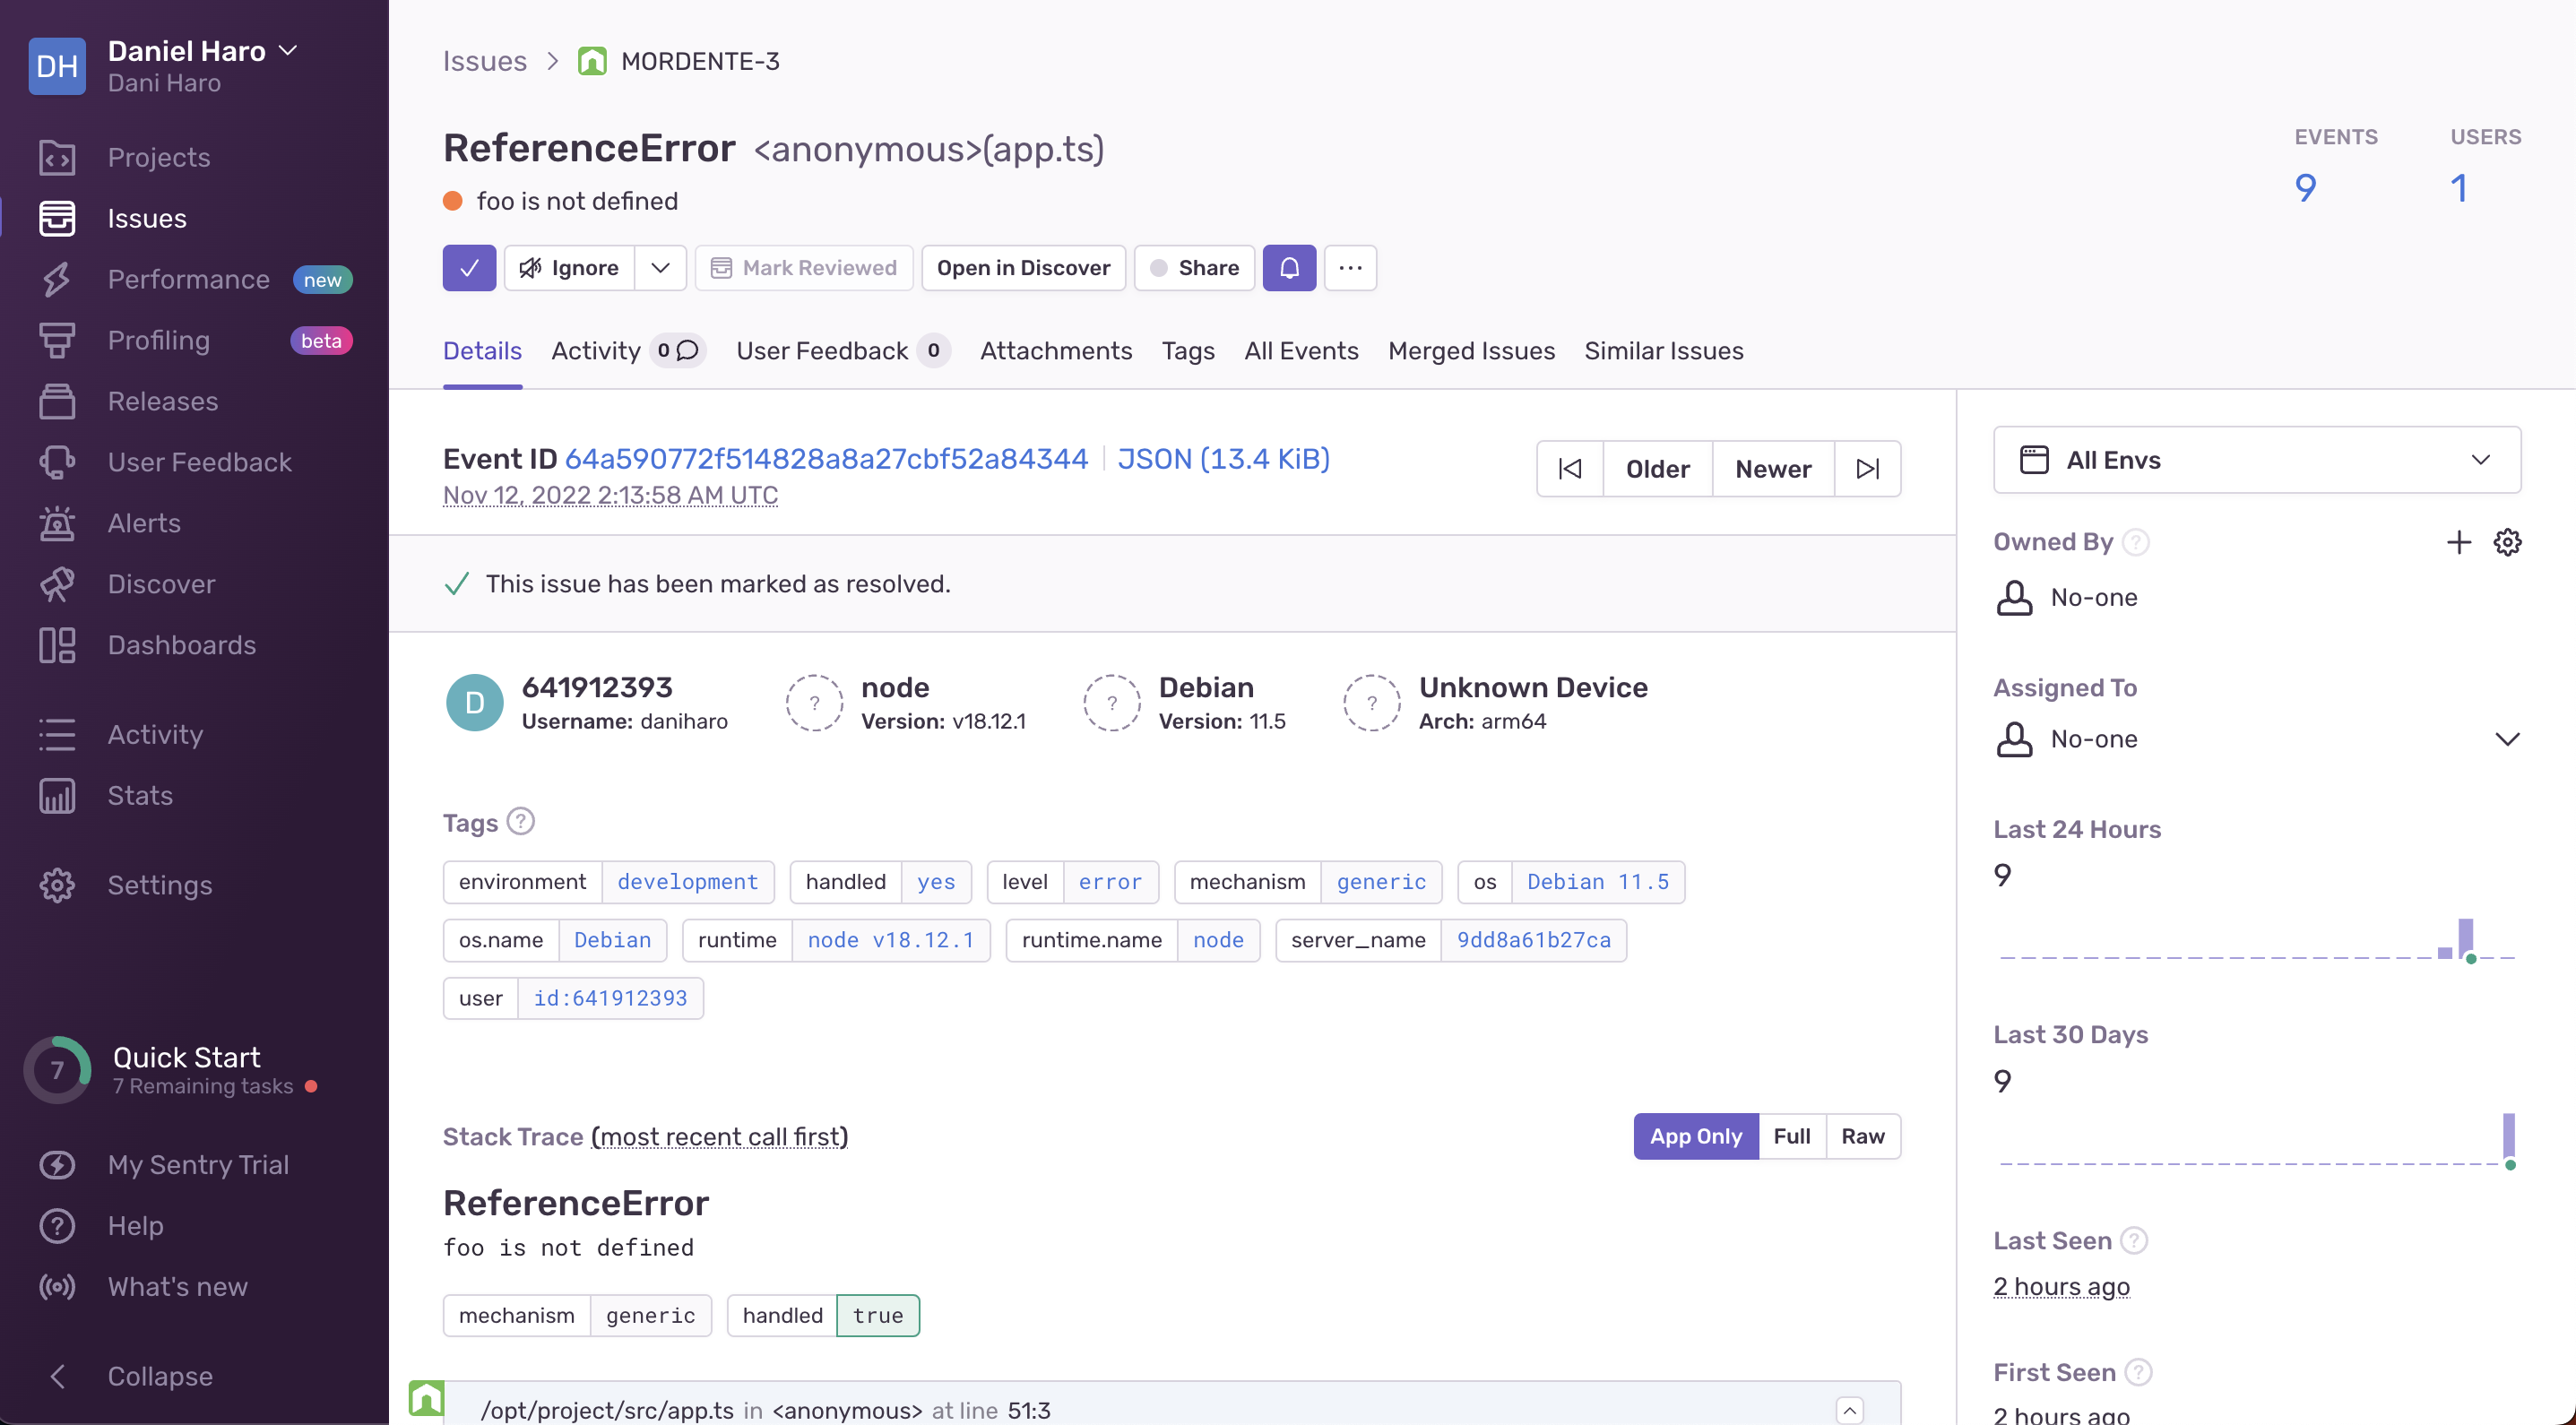
\includegraphics[width=0.75\textwidth]{imagenes/implementacion/sentry_log.png}
\caption{Registro de un error en \textbf{Sentry}}
\label{fig:sentryLog}
\end{figure}

% cuatrimestre 15 semanas

%
\chapter{Pruebas}

% hacer ya DISEÑO PRUEBAS y diseño interfaz

% primera entre el 2 y 4

% segunda 10




% pruebas de usabilidad, (modificaciones) y de software

% net promoter score
% describir participantes, métricas
% describir resultado de cada tarea

Tras el capítulo anterior, ya tenemos una implementación de nuestra herramienta que los usuarios pueden probar para darnos retroalimentación de cara a mejorar la usabilidad de la plataforma.

Las pruebas que se van a realizar en este trabajo, dado que la metodología usada ha sido la del \textit{Design Thinking} y el Diseño Centrado en el Usuario, serán pruebas de usabilidad con usuarios reales.

\section{Diseño de las pruebas}

En esta sección se va a determinar cuál será el diseño de las pruebas de usabilidad. Para ello debemos concretar quién participará en las pruebas, qué tendrán que hacer y qué se les va a preguntar.

\subsection{Participantes}

Para esta primera versión se harán pruebas con 10 personas.

Dado que hay dos roles claramente distinguibles en la aplicación, se seleccionarán 3 administradores y 7 miembros para completar la prueba de usabilidad.


\subsection{Tareas a realizar}

Para comprobar la usabilidad los flujos de trabajo distintos de administradores y miembros, se van a proponer tareas distintas para cada uno de los dos roles.

En el caso de los administradores:

\begin{enumerate}
    \item Crea una agrupación.
    \item Crea un evento.
    \item Edita la descripción de la agrupación.
    \item Sube una obra a la agrupación.
    \item Invita a un miembro de tu banda.
    \item Haz que no pueda unirse nadie más a la agrupación.
    \item Haz administrador al miembro que se ha unido.
    \item Quítale los permisos de administrador al miembro que se ha unido.
    \item Elimina el evento que creaste.
\end{enumerate}

En el caso de los miembros:

\begin{enumerate}
    \item Únete a una agrupación.
    \item Mira los eventos de la agrupación.
    \item Descarga alguna obra de la agrupación.
    \item Sal de la agrupación.
\end{enumerate}


\subsection{Preguntas a realizar}

Las preguntas que se van a realizar a los usuarios son las descritas en la tabla \ref{tab:preguntasPrueba}.

Las relacionadas con tareas concretas nos ayudarán a realizar una mejora de la usabilidad antes de la entrega, solucionando los problemas que manifiesten los usuarios y que se puedan solucionar rápidamente, y planificando como trabajos futuros las soluciones más costosas.

Por otro lado, la primera pregunta genérica nos ayudará a calcular el \textit{NET Promoter Score} o NPS. Según esta herramienta, los encuestados que respondan entre 0 y 6 son detractores, entre 7 y 8 son pasivos y entre 9 y 10 son promotores. De esta forma, se obtendrá un índice realizando el siguiente cálculo:
\[
\textrm{NET} = \frac{\textrm{Promotores} - \textrm{Detractores}}{\textrm{Encuestados}} \times 100
\]

Este índice puede resultar entre -100 y 100. Diremos que tiene un resultado positivo si es mayor a 0, y excelente si es mayor a 50.


\begin{table}[]
    \centering
    \begin{tabular}{|l|c|}
        \hline
        \multicolumn{2}{|c|}{\textbf{Preguntas por tarea}} \\
        \hline
        \textbf{Pregunta} & \textbf{Tipo de respuesta} \\
        \hline
        1. ?`Has podido realizar la tarea? & Sí/No \\
        \hline
        2. ?`Ha sido fácil realizar la tarea? & Entre 1 y 5. \\
        \hline
        \hline
        \multicolumn{2}{|c|}{\textbf{Preguntas genéricas}} \\
        \hline
        \textbf{Pregunta} & \textbf{Tipo de respuesta} \\
        \hline
        1. ?`Algún comentario sobre las tareas? ?`Errores? & Respuesta libre. \\
        \hline
        2. ?`En qué dispositivo has probado el bot? & \makecell{Móvil / \\Ordenador con aplicación / \\ Ordenador en Telegram Web / \\ Otro} \\
        \hline
        3. ?`Opinión sobre la web \texttt{mordente.es}? & \makecell{Entre 0 y 5 para \\ información, diseño adaptativo,\\ apariencia y velocidad} \\
        \hline
        4. ?`Recomendarías Mordente a un amigo? & Entre 0 y 10 \\
        \hline
        5. ?`Tienes algún comentario genérico? & Respuesta libre. \\
        \hline
    \end{tabular}
    \caption{Formulario para la prueba de usabilidad}
    \label{tab:preguntasPrueba}
\end{table}

\section{Realización de las pruebas}


\section{Informe final de las pruebas}

Uno de los problemas detectados durante las pruebas viene derivado por el hecho de que Telegram no obliga a los usuarios a asignarse un nombre de usuario, por lo que el campo \texttt{username} de nuestra base de datos se queda vacío. Esto resultaba en una excepción controlada a la hora de actualizar sus datos que se ha corregido\footnote{\url{https://github.com/daniharo/mordente/commit/70b3b54}}.


\section{Demostración en vídeo}

Se puede visualizar el funcionamiento del bot en el vídeo disponible en este enlace:
\url{}


%
\chapter{Conclusiones y trabajos futuros}

\section{Conclusiones}

% Repasar los objetivos específicos uno por uno,
% resumiendo cómo se han abordado y su grado de
% cumplimiento. Se puede indicar en qué sección de la
% memoria se abordan (un par de páginas).


Llegados a este punto, podemos analizar si hemos cumplido o no los objetivos específicos de este proyecto:

\subsection{Crear una alternativa de aplicación para la gestión de agrupaciones musicales}

El primero de los objetivos trataba de crear una alternativa de software libre que satisficiera las necesidades de las agrupaciones musicales para su gestión. Podemos decir que se ha cumplido, ya que hemos implementado la mayoría de historias de usuario que se propusieron. Además, la mayoría de historias de usuario que no han sido completadas están preparadas para que su implementación no sea de gran dificultad y no haya que rehacer la interfaz de usuario actual.

Los usuarios encuestados en las pruebas con usuarios reales indican que \textbf{Mordente} manifiesta potencial para erigirse como una alternativa sólida al software disponible actualmente.

\subsection{Investigar las posibilidades que ofrece una interfaz de usuario basada en chat}\label{subsection:investigarInterfazChat}

En el capítulo \ref{chapter:diu} explicábamos que este proyecto, al desarrollar una interfaz de usuario sobre un chat de Telegram, ofrece la oportunidad de analizar si la interfaz humano-chat que aporta Telegram es suficiente para realizar tareas de la complejidad de las que se han propuesto.

La respuesta no es rotunda, ya que por un lado para las tareas más simples la interfaz es suficiente, y el hecho de no pedir que los usuarios instalen una aplicación específica disminuye la barrera inicial para la activación de usuarios. Además, se ha descubierto una ventaja que no se había planteado anteriormente: el historial de chats se guarda en el dispositivo, por lo que los usuarios pueden ver información sobre sus agrupaciones cuando no tienen conexión a internet.

Sin embargo, para tareas más complejas los usuarios prefieren tener un panel más completo de forma que se pueda consultar más información necesitando menos pasos para llegar a ella. En esta misma línea, los flujos necesarios para crear agrupaciones, eventos y obras son totalmente secuenciales a modo de conversación, lo cual ha sido visto por los usuarios de forma dispar: aunque sea un flujo natural, no permite modificar fácilmente un paso anterior. De esta forma un formulario estándar sigue siendo conveniente para flujos de creación de elementos.

\subsection{Contribuir a bibliotecas de software libre}

Aparte de publicar este proyecto como ejemplo de bot que integra distintas tecnologías para futuros proyectos parecidos, se han publicado dos bibliotecas que los usuarios de \texttt{grammY} pedían:

\begin{itemize}
    \item \textbf{Adaptador de sesión para \texttt{prisma}} (sección \ref{subsection:adaptadorPrisma}): cerrando un \textit{issue} abierto durante tres meses y ampliamente agradecido por la comunidad, incluso publicado en el canal oficial de Telegram de \texttt{grammY}.
    \item \textbf{Selector de calendario} (sección \ref{subsection:selectorCalendario}): responde a la petición por parte de la comunidad de crear un conjunto de componentes que usan un menú en línea. El selector de calendario es el primero de los componentes que se ha implementado, y su publicación incluso tuvo que ser adelantada dada la cantidad de usuarios pidiendo su implementación.
\end{itemize}


\subsection{Formación en nuevas tecnologías}

Aunque este objetivo no se había planteado inicialmente, se hace importante remarcar la cantidad de tecnologías de actualidad que se han utilizado en este trabajo. La formación en estas tecnologías durante el desarrollo no se limita a la realización de este sino que es totalmente aplicable a trabajos futuros. Entre algunas de las tecnologías que se han aprendido se incluyen \texttt{prisma}, \texttt{grammY}, \texttt{docker}, \texttt{docusaurus}, \texttt{S3}, \texttt{DigitalOcean} o \texttt{Sentry}.



\section{Trabajos futuros}
% Cosas que no se han podido hacer por falta de tiempo o
% restricciones en la tecnología.
% Cosas que no eran objetivos iniciales y se podrían hacer
% en un futuro para mejorar el trabajo (una página).

En esta sección se exponen tareas derivadas del \textit{feedback} recogido de los usuarios o por novedades en las tecnologías durante el desarrollo del trabajo.

\subsection{Función de calendario}

Múltiples usuarios han pedido que se implemente un \textbf{calendario} en el que ver los eventos pasados y próximos de una agrupación. Dado que esta función no la aporta la aplicación que hemos analizado como competencia en la sección \ref{subsection:glissandoo}, se priorizará su implementación como elemento diferenciador.

\subsection{Aplicación web}

Este proyecto se ha dejado preparado para poder implementar en un futuro una aplicación web con la misma funcionalidad que el bot. A nivel de base de datos solo será necesario añadir la información necesaria para el inicio de sesión sin requerir Telegram.

La aplicación web se podría integrar incluso con el bot que hemos desarrollado, de forma que una de las opciones para el inicio de sesión sea obtener un código de inicio de sesión en Telegram.

\subsection{Aplicación web integrada en el bot}

Una de las actualizaciones de la aplicación Telegram que se han lanzado durante el desarrollo de este trabajo incluye la autodenominada \textit{Revolución de los bots}\cite{telegramWebappUpdate}: se trata de la posibilidad de incluir una aplicación web embebida en el bot para tareas que pueden mejorar gracias a su introducción. Una de ellas es la que hemos comentado en la sección \ref{subsection:investigarInterfazChat}: la creación de elementos se beneficia de un formulario tradicional. 

Por ello uno de los trabajos futuros planteados consiste en crear una aplicación web a embeber en el bot que permita, además de crear agrupaciones, eventos y obras, ver un resumen más completo y gráfico de la información interesante para cada usuario, así como la posibilidad de obtener gráficos de asistencia a los eventos y ensayos.

%
%
\nocite{*}
\bibliography{bibliografia/bibliografia}\addcontentsline{toc}{chapter}{Bibliografía}
\bibliographystyle{ieeetr}
%
%\appendix
%\input{apendices/manual_usuario/manual_usuario}
%%\input{apendices/paper/paper}
%\input{glosario/entradas_glosario}
% \addcontentsline{toc}{chapter}{Glosario}
% \printglossary
\chapter*{}
\thispagestyle{empty}

\end{document}
